\chapter{Coupled magneto-elasticity}

\section{Kinematics}

\begin{figure}[h]
\centering
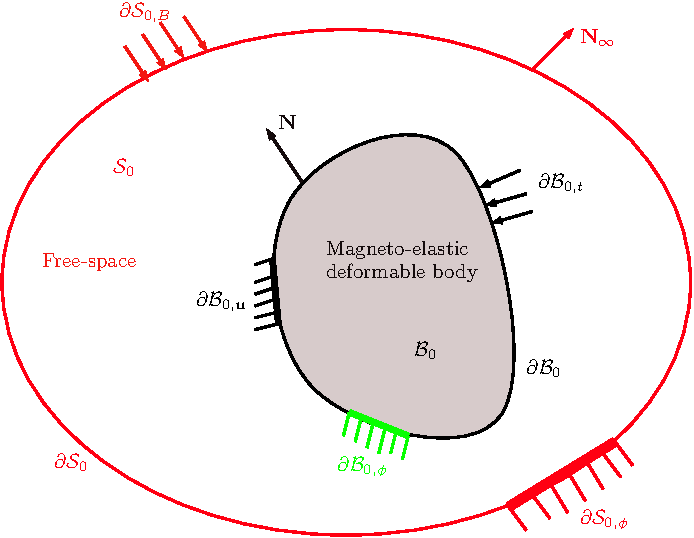
\includegraphics[width=0.6\textwidth]{kinematics_potato_coupled.pdf}
\caption{Domain definition: Deformable magneto-elastic solid $\mathcal{B}_0$ immersed in an electromagnetically permeable free space ($\mathcal{S}_0$).}
\label{fig:3.2}
\end{figure}

We consider a compressible magneto-elastic deformable solid $\mathcal{B}_0$ with a boundary $\partial \mathcal{B}_0$ in a reference state of no stress and no deformations. In this state, the free space surrounding the deformable solid is denoted as $\mathcal{S}_0$ with the topologically constant/fixed boundary $\partial \mathcal{S}_0$. We denote the entire domain containing the magneto-elastic and the surrounding free space domain as $\mathcal{D}_0 := \mathcal{B}_0 \cup \ \mathcal{S}_0$. On application of a combined static mechanical and magnetic load, the body deforms and occupies the current state $\mathcal{B}_t$ with boundary $\partial \mathcal{B}_t$. In the current configuration the free space is denoted as $\mathcal{S}_t$, the free space boundary due to fixed constraints stays constant with $\partial \mathcal{S}_0 = \partial \mathcal{S}_t$ and the entire domain is denoted as $\mathcal{D}_t := \mathcal{B}_t \cup \ \mathcal{S}_t$. Any point in the deformed/current configuration $\mathbf{x} \in \overline{\mathcal{D}_t}$ is identified by a one-to-one non-linear deformation map $\bm{\varphi}$ to $\mathbf{X} \in \overline{\mathcal{D}_0}$ as $\mathbf{x} := \bm{\varphi} (\mathbf{X})$. We define the associated deformation gradient relative to reference configuration $\mathcal{D}_0$ as $\mathbf{F} := \nabla_0 \bm{\varphi}$ and its determinant $J := \text{det} \mathbf{F} > 0$ to ensure that $\bm{\varphi}$ remains invertible and it also avoid the material self-penetration. Here, the gradient w.r.t. $\mathcal{D}_0$ is denoted as $\nabla_0$ and that w.r.t. $\mathcal{D}_t$ is denoted as $\nabla$. $\mathbf{N}$ describes the unit outward normal to $\partial \mathcal{B}_0$ and $\mathbf{N}_{\infty}$ describes the unit outward normal to the boundary $\partial \mathcal{S}_0$. We denote the portion of boundary $\partial \mathcal{B}_{0, \mathbf{u}}$ as the boundary with prescribed deformations and $\partial \mathcal{B}_{0, t}$ as the boundary with prescribed mechanical traction load. The portion $\partial \mathcal{B}_{0, \phi}$ denotes the boundary with prescribed magnetic scalar-valued potential. We assume the boundary $\partial \mathcal{S}_{0,\mathbf{u}} = \partial \mathcal{S}_{0}$ to be prescribed with homogeneous Dirichlet boundary condition for the deformations (fixing the free space boundary topology). We apply a prescribed magnetic scalar-valued potential $\overline{\phi}$ on the portion $\partial \mathcal{S}_{0, \phi}$ to generate a magnetic vector field $\mathbb{H}$ in $\mathcal{D}_0$. Let the associated referential magnetic induction vector be $\mathbb{B}$ and the magnetization vector be $\mathbb{M}$. \par 
We proceed with the assumption that there exists no free electric currents and thus, no electric fields in the complete computational domain. As already explained in detail in Task 1, due to the magnetic vector fields such as $\mathbb{H}$ which is discontinuous over boundaries and material interfaces, for the purpose of finite element modelling we proceed with a magnetic scalar potential formulation. We assume a fictitious quantity $\phi$ and define the curl-free magnetic field $\mathbb{H}$ as \cite{ogden2011mechanics,Dorfmann2014} 
\begin{equation}
\mathbb{H} := -\nabla_0 \phi \ \text{in} \ \mathcal{D}_0.
\label{eq:3.0}
\end{equation}
The continuity condition associated with potential $\phi$ is 
\begin{equation}
\llbracket \phi \rrbracket = 0 \ \text{on} \ \partial\mathcal{B}_{0},
\label{eq:3.0.1}
\end{equation}
and the Dirichlet and Neumann boundary conditions are
\begin{equation}
\phi = \overline{\phi} \ \text{on} \ \partial \mathcal{S}_{0,\phi}, \ \ \mathbb{B}_{\infty} \cdot \mathbf{N}_{\infty} = 0 \ \text{on} \ \partial\mathcal{S}_{0,\mathbb{B}},
\label{eq:3.0.2}
\end{equation}
where $\mathbb{B}_{\infty}$ is the prescribed magnetic induction on the far-field boundary.

\section{Constitutive material model for coupled problem}
The material response is characterised by a Helmholtz free energy density function. For the considered magneto-elastic material, in addition to the dependence on the deformation gradient $\mathbf{F}$ and the Jacobian $J$ (as already seen in quasi-static finite strain compressible elasticity, Task 2.1), the free energy density function now also depends on the referential magnetic vector field. The strain energy function (S.E.F.) is given as: 
\begin{equation}
\Psi = \Psi (J, \mathbf{F}, \mathbb{H}) = \Psi (J, \mathbf{C}, \mathbb{H}).
\label{eq:3.1}
\end{equation}
Using the symmetry argument from the definition of the right Cauchy-Green deformation tensor $\mathbf{C} := \mathbf{F}^T \cdot \mathbf{F}$, the dependence of $\mathbf{F}$ is simplified to a dependence on $\mathbf{C}$. The isotropic hyperelastic material response when $\mathbf{C}$ is used to describe the S.E.F. is given by the constitutive relation as
\begin{equation}
\mathbf{S} = 2 \dfrac{\partial \Psi (J, \mathbf{C}, \mathbb{H})}{\partial \mathbf{C}}.
\label{eq:3.2}
\end{equation}
The referential magnetic induction vector field $\mathbb{B}$ is modelled in terms of the referential magnetic vector field $\mathbb{H}$, taking $\mathbb{H}$ as the independent field
\begin{equation}
\mathbb{B} = \mathbb{B}(\mathbb{H}),
\label{eq:3.3}
\end{equation}
which is termed as the alternative formulation in \cite{dorfmann2004}. With $\mathbb{H}$ chosen as the independent field, its components can be chosen to satisfy the vector equation $\text{Curl} \mathbb{H} = \mathbf{0}$ and then the resulting $\mathbb{B}$ has to satisfy the scalar equation $\text{Div} \mathbb{B} = 0$. This alternative formulation does not put restrictions on the admissible class of constitutive laws (which arise if one were to proceed with $\mathbb{B}$ as the independent field) and also avoids the complexities of a vector-valued magnetic field from the finite element modelling aspects. The fundamental constitutive equation that relates the magnetic quantities $\mathbb{B}, \mathbb{H}$ and the magnetization vector $\mathbb{M}$ is given as \cite{dorfmann2004,dorfmann2005}
\begin{equation}
J^{-1} \mathbf{C} \cdot \mathbb{B} = \mu_0 \left[ \mathbb{H} + \mathbb{M} \right].
\label{eq:3.3.2}
\end{equation}
The magnetization vector field exists only in the solid magneto-elastic material and vanishes in the free space. $\mathbb{B}$ is given by another constitutive relation as \cite{dorfmann2004}: 
\begin{equation}
\mathbb{B} = -\dfrac{\partial \Psi (J, \mathbf{C}, \mathbb{H})}{\partial \mathbb{H}}.
\label{eq:3.4}
\end{equation}
The S.E.F corresponding to a compressible coupled magneto-elastic Neo-Hookean material is given as: 
\begin{align}
\Psi (J, \mathbf{C}, \mathbb{H}) &= \dfrac{\mu}{2} \left[ \mathbf{C} : \mathbf{I} - \mathbf{I} : \mathbf{I} -2 \ln J \right] + \dfrac{\lambda}{2} (\ln J)^2 \textcolor{red}{- \frac{\mu_0 \mu_r}{2} [J \mathbf{C}^{-1} : \mathbb{H} \otimes \mathbb{H}]}, \\
&= \Psi_0^{\text{elas}} (\mathbf{C}) + \mu_r M_0 (J, \mathbf{C}, \mathbb{H}), \\
& \text{with} \ M_0 (J, \mathbf{C}, \mathbb{H}) := -\frac{\mu_0}{2} [J \mathbf{C}^{-1} : \mathbb{H} \otimes \mathbb{H}],
\label{eq:3.5}
\end{align}
where $\mu$ and $\nu$ are the Lam\'e parameters, $\mu_0 = 4 \pi \times 10^{-7} \ \text{Hm}^{-1}$ is the free space (vacuum) magnetic permeability and $\mu_r$ is the relative magnetic permeability of the magneto-elastic material ($\mu_r = 1$ represents the free space material). The term highlighted in red takes into account the energy stored in the body due to applied external magnetic load $\mathbb{H}$ and the response of the coupled interaction between the displacement field and the magnetic field. The term $\Psi_0^{\text{elas}} (\mathbf{C})$ describes the purely elastic response of the material and the term $M_0 (J, \mathbf{C}, \mathbb{H})$ describes the total energy per unit volume stored in the magnetic fields in the free space \cite{dorfmann2004}. The constant $\mu_r > 1$ represents a magnetisable material such as the membrane. \par 

The second Piola-Kirchhoff stress $\mathbf{S}$ for the considered S.E.F. as stated in \Cref{eq:3.5} is derived below.
\begin{align*}
\mathbf{S} &= 2 \dfrac{\partial \Psi (J, \mathbf{C}, \mathbb{H})}{\partial \mathbf{C}} \\
&= 2 \left[ \dfrac{\mu}{2} \left\lbrace \dfrac{\partial [\mathbf{C} : \mathbf{I}]}{\partial \mathbf{C}} - 2 \dfrac{\partial \ln J}{\partial \mathbf{C}} \right\rbrace + \dfrac{\lambda}{2} \dfrac{\partial (\ln J)^2}{\partial \mathbf{C}} - \dfrac{\mu_0 \mu_r}{2} \dfrac{\partial [J \mathbf{C}^{-1} : \mathbb{H} \otimes \mathbb{H}]}{\partial \mathbf{C}} \right]
\end{align*}
Side calculation 1:
\begin{align*}
\dfrac{\partial [\mathbf{C} : \mathbf{I}]}{\partial \mathbf{C}} &= \mathbf{I} \\ 
\dfrac{\partial \ln J}{\partial \mathbf{C}} &= \dfrac{1}{J} \dfrac{\partial J}{\partial \mathbf{C}} \\
\dfrac{\partial (\ln J)^2}{\partial \mathbf{C}} &= 2 \ \ln J \ \dfrac{\partial \ln J}{\partial \mathbf{C}} \\
\dfrac{\partial J}{\partial \mathbf{C}} &= \dfrac{1}{2} J \mathbf{C}^{-1} \ \  \text{c.f. \cite[see][page 46 Equation (3.124)]{Wriggers2008}}
\end{align*}
\begin{align*}
\mathbf{S} &= \mu \mathbf{I} -  \mu \mathbf{C}^{-1} + \lambda \ln J \mathbf{C}^{-1} - \mu_0 \mu_r \dfrac{\partial [J \mathbf{C}^{-1} : \mathbb{H} \otimes \mathbb{H}]}{\partial \mathbf{C}}
\end{align*}
Side calculation 2: Note $\mathbf{C} := \mathbf{F}^T \cdot \mathbf{F} \ $ is symmetric $\implies \mathbf{C}^{-1}$ is also symmetric 
\begin{align*}
\dfrac{\partial [J \mathbf{C}^{-1} : \mathbb{H} \otimes \mathbb{H}]}{\partial \mathbf{C}} &= \dfrac{\partial [J C^{-1}_{IJ} H_I H_J]}{\partial C_{KL}} \ \mathbf{E}_K \otimes \mathbf{E}_L \\
&= C^{-1}_{IJ} \ H_I \ H_J \ \dfrac{\partial J}{\partial C_{KL}} \ \mathbf{E}_K \otimes \mathbf{E}_L + J \ H_I \ H_J \ \dfrac{\partial C^{-1}_{IJ}}{\partial C_{KL}} \ \mathbf{E}_K \otimes \mathbf{E}_L \\
&= C^{-1}_{IJ} \ H_I \ H_J \ \dfrac{J}{2} \ C^{-1}_{KL} \ \mathbf{E}_K \otimes \mathbf{E}_L + J \ H_I \ H_J \  \dfrac{\partial C^{-1}_{IJ}}{\partial C_{KL}} \ \mathbf{E}_K \otimes \mathbf{E}_L
\end{align*}
c.f. \cite[see][page 519]{Wriggers2008}: 
\begin{align*}
\dfrac{\partial C^{-1}_{IJ}}{\partial C_{KL}} = -\dfrac{1}{2} [C^{-1}_{IK} \ C^{-1}_{LJ} + C^{-1}_{IL} \ C^{-1}_{KJ}]
\end{align*}
\begin{align*}
\dfrac{\partial [J \mathbf{C}^{-1} : \mathbb{H} \otimes \mathbb{H}]}{\partial \mathbf{C}} &= \dfrac{J}{2} C^{-1}_{IJ} H_I H_J C^{-1}_{KL} \mathbf{E}_K \otimes \mathbf{E}_L + \dfrac{-J}{2} \left[ C^{-1}_{IK} C^{-1}_{LJ} H_I H_J + C^{-1}_{IL} C^{-1}_{KJ} H_I H_J \right] \mathbf{E}_K \otimes \mathbf{E}_L \\
&= \dfrac{J}{2} C^{-1}_{IJ} H_I H_J C^{-1}_{KL} \mathbf{E}_K \otimes \mathbf{E}_L - \dfrac{J}{2} \left[ C^{-1}_{KI} H_I C^{-1}_{LJ} H_J + C^{-1}_{LI} H_I C^{-1}_{KJ} H_J \right] \mathbf{E}_K \otimes \mathbf{E}_L \\
&= \dfrac{J}{2} \ C^{-1}_{IJ} \ H_I \ H_J \ C^{-1}_{KL} \ \mathbf{E}_K \otimes \mathbf{E}_L - J [C^{-1}_{KI} \ H_I \ C^{-1}_{LJ} \ H_J]^{sym} \ \mathbf{E}_K \otimes \mathbf{E}_L \\
&= \dfrac{J}{2} [ \mathbf{C}^{-1} : \mathbb{H} \otimes \mathbb{H}] \mathbf{C}^{-1} - J [ (\mathbf{C}^{-1} \cdot \mathbb{H}) \otimes (\mathbf{C}^{-1} \cdot \mathbb{H})]^{sym}
\end{align*}
\begin{empheq}[box=\tcbhighmath]{align}
\mathbf{S} = & \ \mu \mathbf{I} - [\mu - \lambda \ln J] \mathbf{C}^{-1} - \dfrac{\mu_0 \mu_r}{2} \ J \ [ \mathbf{C}^{-1} : \mathbb{H} \otimes \mathbb{H}] \mathbf{C}^{-1} \nonumber \\
&+ \mu_0 \mu_r \ J \ [ (\mathbf{C}^{-1} \cdot \mathbb{H}) \otimes (\mathbf{C}^{-1} \cdot \mathbb{H})]^{sym}
\label{eq:3.6}
\end{empheq}

The referential magnetic induction vector field is given as:
\begin{align*}
\mathbb{B} &= - \dfrac{\partial \Psi (J, \mathbf{C}, \mathbb{H})}{\partial \mathbb{H}} \\
&= \dfrac{\mu_0 \mu_r}{2} \dfrac{\partial [J \ \mathbf{C}^{-1} : \mathbb{H} \otimes \mathbb{H}]}{\partial \mathbb{H}} \\
&= \dfrac{\mu_0 \mu_r}{2} \dfrac{\partial [J \ C^{-1}_{IJ} \ H_I \ H_J	]}{\partial H_K} \mathbf{E}_K \\
&= \dfrac{\mu_0 \mu_r}{2} \left[ J \ C^{-1}_{IJ} \dfrac{\partial H_I}{\partial H_K} \ H_J + J \ C^{-1}_{IJ} \ H_I \dfrac{\partial H_J}{\partial H_K} \right] \mathbf{E}_K \\
&= \dfrac{\mu_0 \mu_r}{2} \left[ J \ C^{-1}_{IJ} \ \delta_{IK} \ H_J + J \ C^{-1}_{IJ} \ H_I \ \delta_{JK} \right] \mathbf{E}_K \\
&= \dfrac{\mu_0 \mu_r}{2} \left[ J \ C^{-1}_{JI} \ \delta_{IK} \ H_J + J \ C^{-1}_{IJ} \ \delta_{JK} \ H_I \right] \mathbf{E}_K \\
&= \dfrac{\mu_0 \mu_r}{2} \left[ J \ C^{-1}_{JK} \ H_J + J \ C^{-1}_{IK} \ H_I \right] \mathbf{E}_K \\
&= \dfrac{\mu_0 \mu_r}{2} \left[ J \ C^{-1}_{KJ} \ H_J + J \ C^{-1}_{KI} \ H_I \right] \mathbf{E}_K
\end{align*}
\begin{empheq}[box=\tcbhighmath]{align}
\mathbb{B} = \mu_0 \mu_r \ J \ [\mathbf{C}^{-1} \cdot \mathbb{H}]
\label{eq:3.7}
\end{empheq}
The referential material elasticity tangent $\mathfrak{C}$ is defined as 
\begin{equation}
\mathfrak{C} := 2 \dfrac{\partial \mathbf{S}(J, \mathbf{C}, \mathbb{H})}{\partial \mathbf{C}} = 4 \dfrac{\partial^2 \Psi (J, \mathbf{C}, \mathbb{H})}{\partial \mathbb{C} \otimes \partial \mathbf{C}}.
\label{eq:3.8}
\end{equation} 
Using the result of \Cref{eq:3.6}, $\mathfrak{C}$ is derived as follows.
\begin{align*}
\mathfrak{C} &= 2 \dfrac{\partial \mathbf{S}}{\partial \mathbf{C}} \\
&= 2 \dfrac{\partial S_{KL}}{\partial C_{MN}} \ \mathbf{E}_K \otimes \mathbf{E}_L \otimes \mathbf{E}_M \otimes \mathbf{E}_N \\
\begin{split}
=\ & 2 \left\lbrace - \mathbf{C}^{-1} \otimes \dfrac{\partial [\mu - \lambda \ln J]}{\partial \mathbf{C}} - [\mu - \lambda \ln J] \dfrac{\partial \mathbf{C}^{-1}}{\partial \mathbf{C}} - \dfrac{\mu_0 \mu_r}{2} [\mathbf{C}^{-1} : \mathbb{H} \otimes \mathbb{H}] \ \mathbf{C}^{-1} \otimes \dfrac{\partial J}{\partial \mathbf{C}} \right\rbrace \\
&+ 2 \left\lbrace - \dfrac{\mu_0 \mu_r}{2} \ J \ \mathbf{C}^{-1} \otimes \dfrac{\partial [\mathbf{C}^{-1} : \mathbb{H} \otimes \mathbb{H}]}{\partial \mathbf{C}} - \dfrac{\mu_0 \mu_r}{2} \ J \ [\mathbf{C}^{-1} : \mathbb{H} \otimes \mathbb{H}] \dfrac{\partial \mathbf{C}^{-1}}{\partial \mathbf{C}} \right\rbrace \\
&+ 2 \left\lbrace \mu_0 \mu_r [ (\mathbf{C}^{-1} \cdot \mathbb{H}) \otimes (\mathbf{C}^{-1} \cdot \mathbb{H})]^{sym} \otimes \dfrac{\partial J}{\partial \mathbf{C}} + \mu_0 \mu_r \ J \ \dfrac{\partial [ (\mathbf{C}^{-1} \cdot \mathbb{H}) \otimes (\mathbf{C}^{-1} \cdot \mathbb{H})]^{sym}}{\partial \mathbf{C}} \right\rbrace
\end{split} \\
\begin{split}
=\ & 2 \left\lbrace C^{-1}_{KL} \ \dfrac{\lambda}{J} \dfrac{\partial J}{\partial C_{MN}} - [\mu - \lambda \ln J] \left\lbrace \dfrac{-1}{2} \left( C^{-1}_{KM} \ C^{-1}_{NL} + C^{-1}_{KN} \ C^{-1}_{ML} \right) \right\rbrace \right\rbrace \\
& \ \ \mathbf{E}_K \otimes \mathbf{E}_L \otimes \mathbf{E}_M \otimes \mathbf{E}_N\\
&+ 2 \left\lbrace - \dfrac{\mu_0 \mu_r}{2} \ [C^{-1}_{IJ} \ H_I \ H_J] C^{-1}_{KL} \dfrac{1}{2} \ J \ C^{-1}_{MN} - \dfrac{\mu_0 \mu_r}{2} J \ C^{-1}_{KL} \dfrac{\partial [C^{-1}_{IJ} \ H_I \ H_J]}{\partial C_{MN}} \right\rbrace \\
& \ \ \mathbf{E}_K \otimes \mathbf{E}_L \otimes \mathbf{E}_M \otimes \mathbf{E}_N \\
&+ 2 \left\lbrace - \dfrac{\mu_0 \mu_r}{2} \ J \ [C^{-1}_{IJ} \ H_I \ H_J] \left\lbrace \dfrac{-1}{2} (C^{-1}_{KM} \ C^{-1}_{NL} + C^{-1}_{KN} \ C^{-1}_{ML}) \right\rbrace \right\rbrace \mathbf{E}_K \otimes \mathbf{E}_L \otimes \mathbf{E}_M \otimes \mathbf{E}_N \\
&+ 2 \left\lbrace \mu_0 \mu_r [C^{-1}_{KI} \ H_I \ C^{-1}_{LJ} \ H_J]^{sym} \ \dfrac{1}{2} J \ C^{-1}_{MN} + \mu_0 \mu_r \ J \ \dfrac{\partial [C^{-1}_{KI} \ H_I \ C^{-1}_{LJ} \ H_J]^{sym}}{\partial C_{MN}} \right\rbrace \\
& \ \ \mathbf{E}_K \otimes \mathbf{E}_L \otimes \mathbf{E}_M \otimes \mathbf{E}_N
\end{split}\\
\begin{split}
=\ & \lambda \ C^{-1}_{KL} \ C^{-1}_{MN} + [\mu - \lambda \ln J] \left( C^{-1}_{KM} \ C^{-1}_{NL} + C^{-1}_{KN} \ C^{-1}_{ML} \right) - \dfrac{\mu_0 \mu_r}{2} \ J \ [C^{-1}_{IJ} \ H_I \ H_J] C^{-1}_{KL} \ C^{-1}_{MN}  \\
&- \mu_0 \mu_r J \ C^{-1}_{KL} \ \dfrac{\partial [C^{-1}_{IJ} \ H_I \ H_J]}{\partial C_{MN}} + \dfrac{\mu_0 \mu_r}{2} \ J \ [C^{-1}_{IJ} \ H_I \ H_J] (C^{-1}_{KM} \ C^{-1}_{NL} + C^{-1}_{KN} \ C^{-1}_{ML}) \\
&+ \mu_0 \mu_r \ J \ [C^{-1}_{KI} \ H_I \ C^{-1}_{LJ} \ H_J]^{sym} \ C^{-1}_{MN} + 2 \mu_0 \mu_r \ J \ \dfrac{\partial [C^{-1}_{KI} \ H_I \ C^{-1}_{LJ} \ H_J]^{sym}}{\partial C_{MN}} \\
& \ \ \mathbf{E}_K \otimes \mathbf{E}_L \otimes \mathbf{E}_M \otimes \mathbf{E}_N
\end{split}\\
\end{align*}
Side calculation 1:
\begin{align*}
\dfrac{\partial [C^{-1}_{IJ} \ H_I \ H_J]}{\partial C_{MN}} &= H_I \ H_J \ \dfrac{\partial C^{-1}_{IJ}}{\partial C_{MN}}\\
&= \dfrac{-1}{2} \ H_I \ H_J \ [C^{-1}_{IM} \ C^{-1}_{NJ} + C^{-1}_{IN} \ C^{-1}_{MJ}]\\
&= \dfrac{-1}{2} [C^{-1}_{MI} \ H_I \ C^{-1}_{NJ} \ H_J + C^{-1}_{NI} \ H_I \ C^{-1}_{MJ} \ H_J]\\
&= - [C^{-1}_{MI} \ H_I \ C^{-1}_{NJ} \ H_J]^{sym}\\
&= - [ (\mathbf{C}^{-1} \cdot \mathbb{H}) \otimes (\mathbf{C}^{-1} \cdot \mathbb{H}) ]^{sym}
\end{align*}
Side calculation 2:
\begin{align*}
\dfrac{\partial [C^{-1}_{KI} \ H_I \ C^{-1}_{LJ} \ H_J]^{sym}}{\partial C_{MN}} &= \dfrac{1}{2} \dfrac{\partial \left[ C^{-1}_{KI} \ H_I \ C^{-1}_{LJ} \ H_J + C^{-1}_{LI} \ H_I \ C^{-1}_{KJ} \ H_J \right] }{\partial C_{MN}}\\
\begin{split}
= & \ \dfrac{1}{2} \dfrac{\partial C^{-1}_{KI}}{\partial C_{MN}} \ H_I \ C^{-1}_{LJ} \ H_J + \dfrac{1}{2} C^{-1}_{KI} \ H_I \ \dfrac{\partial C^{-1}_{LJ}}{\partial C_{MN}} \ H_J \\
&+ \dfrac{1}{2} \dfrac{\partial C^{-1}_{LI}}{\partial C_{MN}} \ H_I \ C^{-1}_{KJ} \ H_J + \dfrac{1}{2} C^{-1}_{LI} \ H_I \ \dfrac{\partial C^{-1}_{KJ}}{\partial C_{MN}} \ H_J \\
\end{split}\\
\begin{split}
= & \ \dfrac{1}{2} \dfrac{-1}{2} \left[ C^{-1}_{KM} C^{-1}_{NI} + C^{-1}_{KN} C^{-1}_{MI} \right] \ H_I \ C^{-1}_{LJ} \ H_J \\
&+ \ \dfrac{1}{2} \dfrac{-1}{2} C^{-1}_{KI} \ H_I \left[ C^{-1}_{LM} C^{-1}_{NJ} + C^{-1}_{LN} C^{-1}_{MJ} \right] \ H_J \\
&+ \ \dfrac{1}{2} \dfrac{-1}{2} \left[ C^{-1}_{LM} C^{-1}_{NI} + C^{-1}_{LN} C^{-1}_{MI} \right] \ H_I \ C^{-1}_{KJ} \ H_J \\
&+ \ \dfrac{1}{2} \dfrac{-1}{2} C^{-1}_{LI} \ H_I \left[ C^{-1}_{KM} C^{-1}_{NJ} + C^{-1}_{KN} C^{-1}_{MJ} \right] \ H_J \\
\end{split}\\
\begin{split}
= &- \textcolor{blue}{\dfrac{1}{4} \left[ C^{-1}_{KM} \ C^{-1}_{NI} \ H_I \ C^{-1}_{LJ} \ H_J + C^{-1}_{KN} \ C^{-1}_{MI} \ H_I \ C^{-1}_{LJ} \ H_J \right]} \\
&- \textcolor{red}{\dfrac{1}{4} \left[ C^{-1}_{KI} \ H_I \ C^{-1}_{LM} \ C^{-1}_{NJ} \ H_J + C^{-1}_{KI} \ H_I \ C^{-1}_{LN} \ C^{-1}_{MJ} \ H_J \right]} \\
&- \textcolor{blue}{\dfrac{1}{4} \left[ C^{-1}_{LM} \ C^{-1}_{NI} \ H_I \ C^{-1}_{KJ} \ H_J + C^{-1}_{LN} \ C^{-1}_{MI} \ H_I \ C^{-1}_{KJ} \ H_J \right]} \\
&- \textcolor{red}{\dfrac{1}{4} \left[ C^{-1}_{LI} \ H_I \ C^{-1}_{KM} \ C^{-1}_{NJ} \ H_J + C^{-1}_{LI} \ H_I \ C^{-1}_{KN} \ C^{-1}_{MJ} \ H_J \right]}\\
\end{split}\\
&= -\textcolor{red}{\mathbb{X}} - \textcolor{blue}{\mathbb{Y}}
\end{align*}
The tensors
\begin{align*}
\textcolor{red}{\mathbb{X}} &:= \dfrac{1}{4} \left[ C^{-1}_{KI} H_I C^{-1}_{LM} C^{-1}_{NJ} H_J + C^{-1}_{KI} H_I C^{-1}_{LN} C^{-1}_{MJ} H_J + C^{-1}_{LI} H_I C^{-1}_{KM} C^{-1}_{NJ} H_J + C^{-1}_{LI} H_I C^{-1}_{KN} C^{-1}_{MJ} H_J \right]\\
\textcolor{blue}{\mathbb{Y}} &:= \dfrac{1}{4} \left[ C^{-1}_{KM} C^{-1}_{NI} H_I C^{-1}_{LJ} H_J + C^{-1}_{KN} C^{-1}_{MI} H_I C^{-1}_{LJ} H_J + C^{-1}_{LM} C^{-1}_{NI} H_I C^{-1}_{KJ} H_J + C^{-1}_{LN} C^{-1}_{MI} H_I C^{-1}_{KJ} H_J \right]
\end{align*}
\noindent with indices $\mathbf{E}_K \otimes \mathbf{E}_L \otimes \mathbf{E}_M \otimes \mathbf{E}_N$ are both symmetric rank-4 tensors such that for given symmetric rank-2 tensors $\mathbf{M}, \mathbf{N}, \mathbf{P}, \mathbf{Q}$, we have:
\begin{align*}
\mathbf{N} &= \textcolor{red}{\mathbb{X}} : \mathbf{M}, \\
\mathbf{Q} &= \textcolor{blue}{\mathbb{Y}} : \mathbf{P}.
\end{align*}
\begin{align*}
\mathfrak{C} =  & \ \lambda \ \mathbf{C}^{-1} \otimes \mathbf{C}^{-1} -2 [\mu - \lambda \ln J] \ \dfrac{\partial \mathbf{C}^{-1}}{\partial \mathbf{C}} \\
&- \dfrac{\mu_0 \mu_r}{2} \ J \ [\mathbf{C}^{-1} : \mathbb{H} \otimes \mathbb{H}] (\mathbf{C}^{-1} \otimes \mathbf{C}^{-1}) + \mu_0 \mu_r \ J \ (\mathbf{C}^{-1} \otimes [ (\mathbf{C}^{-1} \cdot \mathbb{H}) \otimes (\mathbf{C}^{-1} \cdot \mathbb{H}) ]^{sym}) \\
&- \mu_0 \mu_r \ J \ [\mathbf{C}^{-1} : \mathbb{H} \otimes \mathbb{H}] \ \dfrac{\partial \mathbf{C}^{-1}}{\partial \mathbf{C}} + \mu_0 \mu_r \ J \ ([ (\mathbf{C}^{-1} \cdot \mathbb{H}) \otimes (\mathbf{C}^{-1} \cdot \mathbb{H}) ]^{sym} \otimes \mathbf{C}^{-1}) \\
&- 2 \mu_0 \mu_r \ J \ (\textcolor{red}{\mathbb{X}} + \textcolor{blue}{\mathbb{Y}})
\end{align*}
For given symmetric rank 2 tensors $\mathbf{A}$ and $\mathbf{B}$, we know: $\mathbf{A} \otimes \mathbf{B} = \mathbf{B} \otimes \mathbf{A}.$
\begin{empheq}[box=\tcbhighmath]{align}
\mathfrak{C} = & \ \lambda \ \mathbf{C}^{-1} \otimes \mathbf{C}^{-1} -2 [\mu - \lambda \ln J] \ \dfrac{\partial \mathbf{C}^{-1}}{\partial \mathbf{C}} \nonumber \\
&- \dfrac{\mu_0 \mu_r}{2} \ J \ [\mathbf{C}^{-1} : \mathbb{H} \otimes \mathbb{H}] (\mathbf{C}^{-1} \otimes \mathbf{C}^{-1}) - \mu_0 \mu_r \ J \ [\mathbf{C}^{-1} : \mathbb{H} \otimes \mathbb{H}] \ \dfrac{\partial \mathbf{C}^{-1}}{\partial \mathbf{C}} \nonumber \\
&+ 2 \mu_0 \mu_r \ J \ (\mathbf{C}^{-1} \cdot \mathbb{H}) \otimes (\mathbf{C}^{-1} \cdot \mathbb{H}) ]^{sym} \otimes \mathbf{C}^{-1}) - 2 \mu_0 \mu_r \ J \ (\textcolor{red}{\mathbb{X}} + \textcolor{blue}{\mathbb{Y}})
\label{eq:3.9}
\end{empheq}
The fourth-order referential material elasticity tensor possess both major and minor symmetries, i.e. $\mathfrak{C} = C_{KLMN} = C_{MNKL} = C_{KLNM} = C_{LKMN}$.

\section{Problem set up}
\label{sec:problem_setup}

\subsection{Set up for the magnetic field $\mathbb{H}$}
Following the results obtained in Task 1 and Task 2.1, the problem set up for the coupled magneto-elasticity problem is updated in view of modelling the instabilities arising in the torus membrane. Same geometry of the axisymmetric torus membrane immersed in free space is used as in the Task 1 and Task 2.1.  \par 

\begin{figure}[h]
\centering
\begin{subfigure}{0.59\textwidth}
\centering
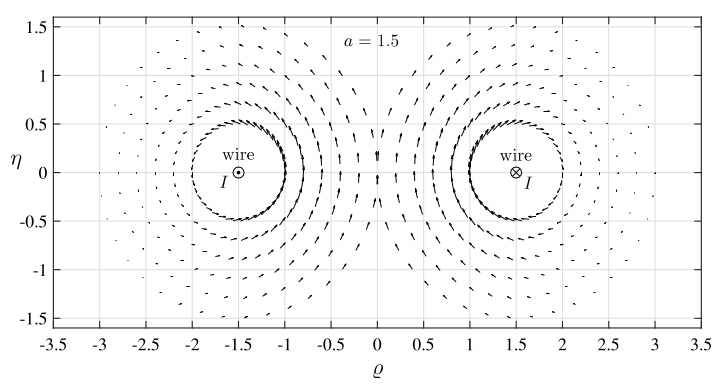
\includegraphics[width=0.9\textwidth]{magnetic_field_saxena.png}
\caption{Desired distribution \cite{reddy_toroid}}
\label{fig:3.3.1}
\end{subfigure}
\begin{subfigure}{0.39\textwidth}
\centering
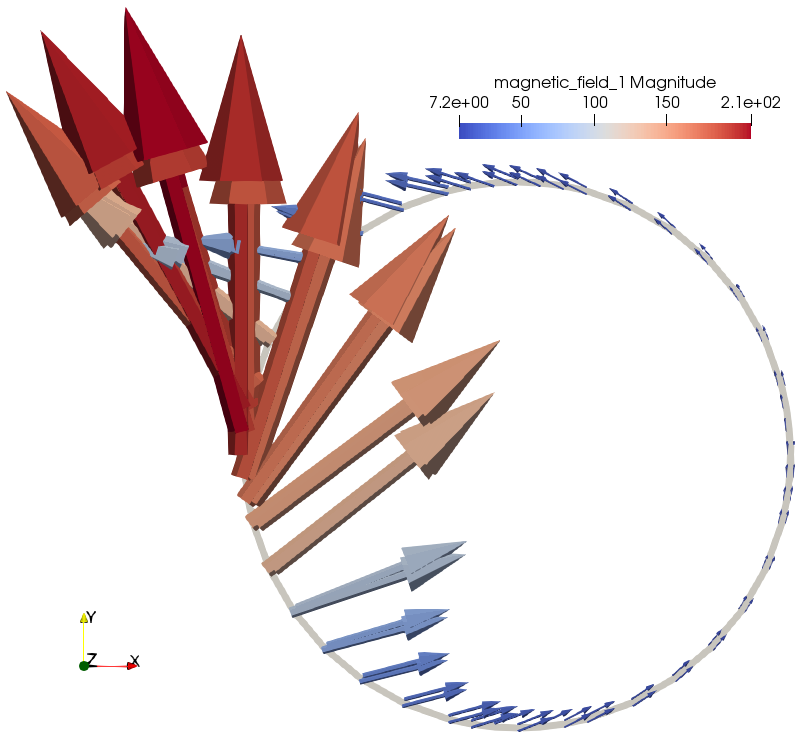
\includegraphics[width=0.95\textwidth]{2d_toroid_field_2.png}
\caption{Modelled distribution}
\label{fig:3.3.2}
\end{subfigure}
\caption{Resulting magnetic field in torus membrane}
\label{fig:3.3}
\end{figure}

In Task 1 of the thesis (a purely magneto-static problem), we considered a rectangular permanent magnet placed at the center and along the axis of symmetry to generate a circulating magnetic field $\mathbb{H}$ in $\mathcal{D}_0$. A linearly varying potential function was applied to this permanent magnet region, c.f. \Cref{fig:3.4.1}. The dimension of this rectangular permanent magnet region and the potential difference per unit length to be applied were taken as user input parameters. It was observed in the results for Task 1 that the size of the magnet and the potential applied influenced the resulting magnetic field generated in the domain. A small study for this was also carried out and presented in Task 1. The important finding of this study was that the direction of the resulting magnetic field in the tours membrane did not change irrespective of increasing the magnet size and the applied potential value. The resulting magnetic field, c.f. \Cref{fig:3.3.2}, in the torus membrane on the left section (in close proximity to the permanent magnet and axis of symmetry) was comparatively high in magnitude than on the other sections of the membrane. The orientation of this large magnetic field on the left section was the same as that observed on the right section. The orientation of the magnetic field did not meet the desired result as observed in \Cref{fig:3.3.1} from \cite{reddy_toroid}. The main reason for this discrepancy was the different modelling approach taken by us to generate the magnetic field compared to the approach taken in \cite{reddy_toroid}. In \cite{reddy_toroid}, a thin current carrying wire placed along the centre line of the torus membrane was considered to generate the field $\mathbb{H}$. This approach is not possible from the perspective of finite element modelling and thus we had employed a permanent magnet region to generate a similar effect. \par 

\begin{figure}[h]
\centering
\begin{subfigure}{0.35\textwidth}
\centering
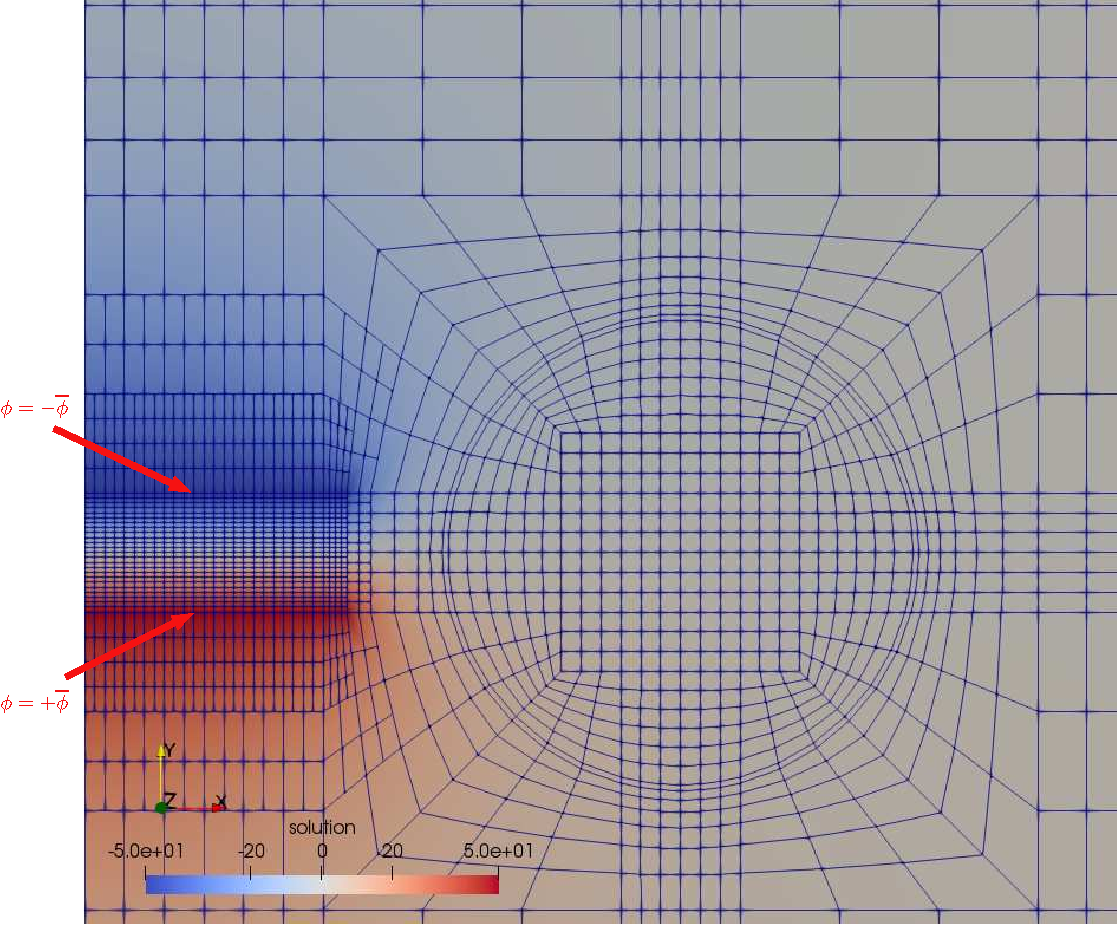
\includegraphics[width=0.9\textwidth]{applied_mag_pot_magnet.pdf}
\caption{Permanent magnet used in Task 1 (purely magneto-static problem)}
\label{fig:3.4.1}
\end{subfigure}
\begin{subfigure}{0.5\textwidth}
\centering
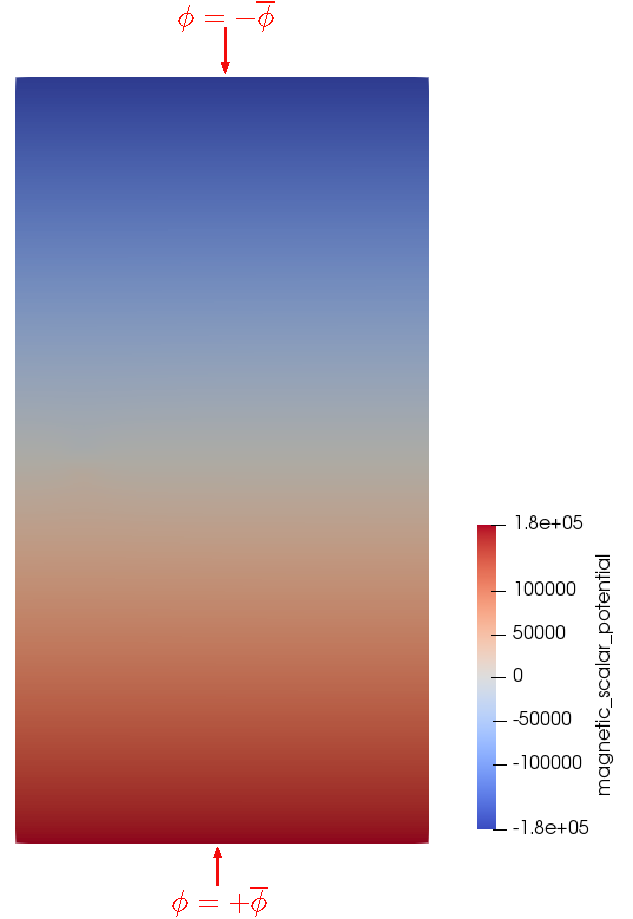
\includegraphics[width=0.7\textwidth]{magnetic_potential_coupled_problem.pdf}
\caption{For the coupled problem}
\label{fig:3.4.2}
\end{subfigure}
\caption{Applied potential difference per unit length}
\label{fig:3.4}
\end{figure}

\begin{figure}[h!]
\centering
\begin{subfigure}{0.59\textwidth}
\centering
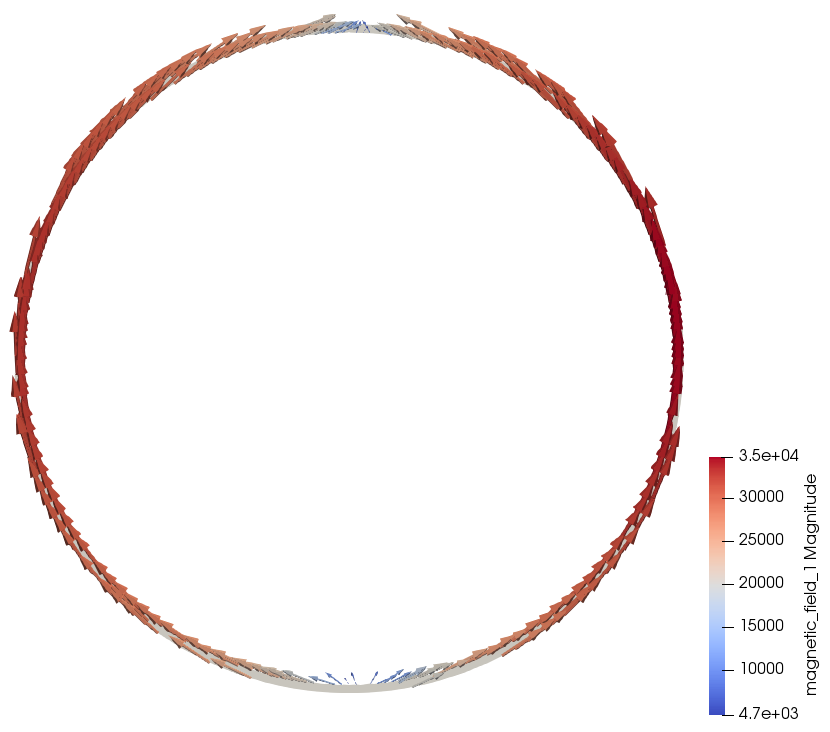
\includegraphics[width=0.8\textwidth]{magnetic_field_toroid_coupled.png}
\caption{Modelled distribution of $\mathbb{H}$ in torus membrane}
\label{fig:3.5.1}
\end{subfigure}
\begin{subfigure}{0.39\textwidth}
\centering
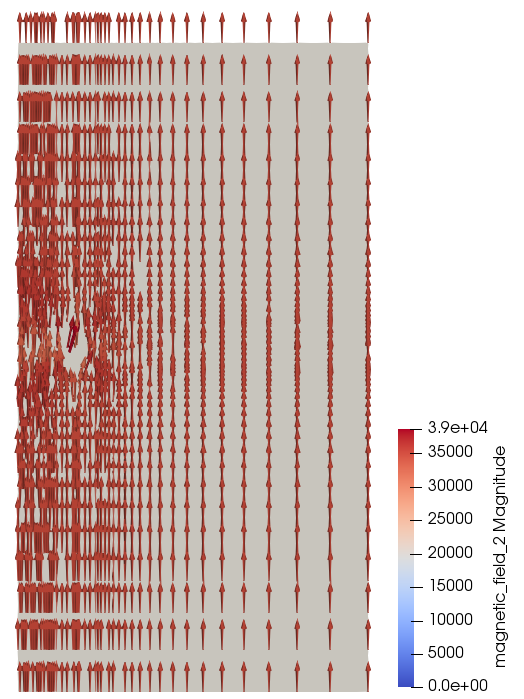
\includegraphics[width=0.85\textwidth]{magnetic_field_50.png}
\caption{Uniformly distributed magnetic field in $\mathcal{D}_0$}
\label{fig:3.5.2}
\end{subfigure}
\caption{Resulting magnetic field $\mathbb{H}$ for the coupled problem (Vectors are coloured and scaled to the magnitude of the magnetic field $\mathbb{H}$)}
\label{fig:3.5}
\end{figure}

Due to such a concentrated magnetic field on one section of the membrane, modelling of instabilities arising from the coupled  mechanical and magnetic static loading would not be possible. The instability behaviour of our interest is witnessed at large mechanical loads and under an uniformly distributed magnetic field of large magnitude \cite{reddy_toroid,Reddy2018}. Thus, to generate a uniformly distributed magnetic field in the coupled problem and to study the instabilities, a different approach was undertaken. In the new approach, we considered the top and bottom boundary of the free space $\partial \mathcal{S}_0$ as the south and the north pole of a permanent magnet, respectively. A constant potential $\overline{\phi}$ of same magnitude but opposite polarities was prescribed at the top and the bottom boundary as observed in \Cref{fig:3.4.2}. The resulting magnetic field in \Cref{fig:3.5.2} is uniformly distributed and vertically aligned. The important outcome of this approach, comparing \Cref{fig:3.5.1} to \Cref{fig:3.3.2}, is the absence of a concentrated magnetic field of high magnitude on any section of the tours membrane. Using the new approach we were able to generate a uniform magnetic field in the torus membrane. This will prove ideal to study the instability behaviour under a quasi-static mechanical load. \par 

\subsection{Problem geometry and load application set up}
\label{sec:load_setup}

\begin{figure}[h]
\centering
\begin{subfigure}{0.55\textwidth}
\centering
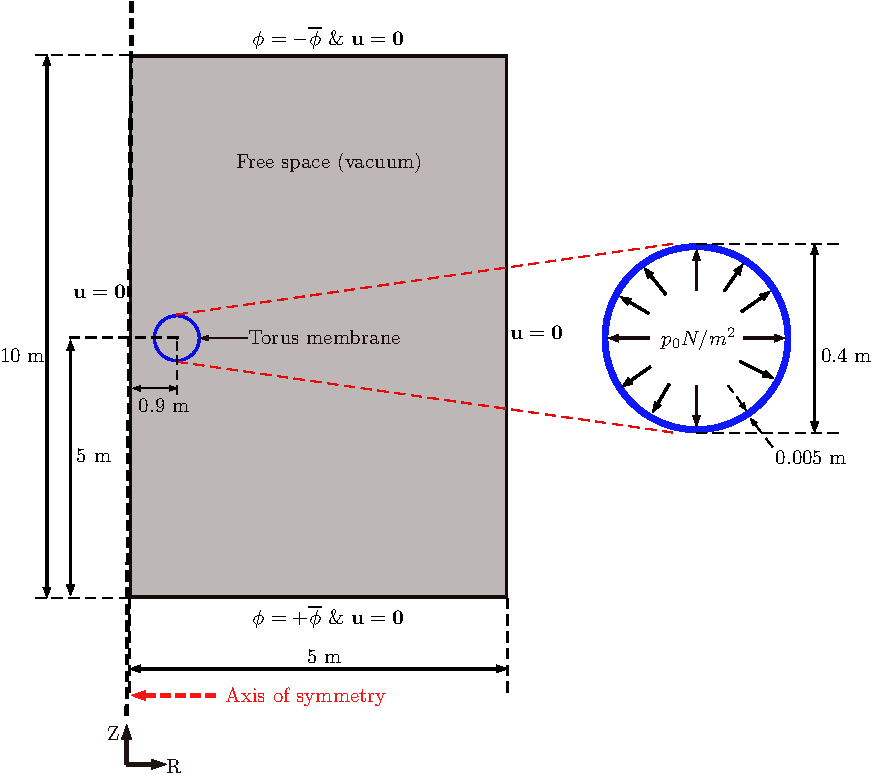
\includegraphics[width=0.95\textwidth]{coupled_prob_description.pdf}
\caption{Representative geometry description}
\label{fig:3.6.1}
\end{subfigure}
\begin{subfigure}{0.44\textwidth}
\centering
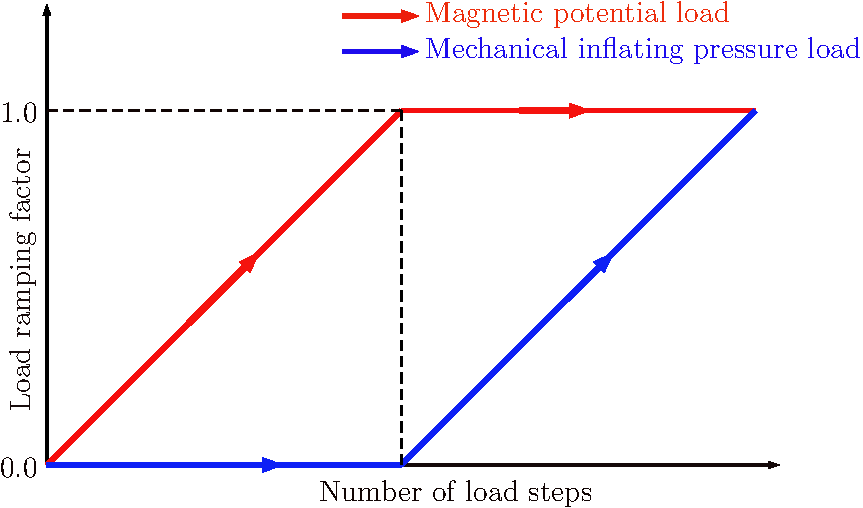
\includegraphics[width=0.95\textwidth]{load_cycle.pdf}
\caption{Load application cycle}
\label{fig:3.6.2}
\end{subfigure}
\caption{Coupled problem geometry and applied load set up}
\label{fig:3.6}
\end{figure}

The problem geometry shown in \Cref{fig:3.6.1} is same as used in Task 1 and Task 2.1. However, now along with the finite elastic deformations of the circular cross-section torus membrane, we also model the magnetic scalar potential problem and study the coupled finite strain magneto-elastic deformations of this membrane immersed in the surrounding free space. The interactions between the displacement and magnetic fields and the response of the material for the coupled loads will be examined. We consider the external load application in uniformly increasing load steps as shown in \Cref{fig:3.6.2}. For the study of instabilities arising due to coupled loads, following \cite{reddy_toroid}, we first apply the scalar magnetic potential load $\phi = \overline{\phi}$ on the far-field free space boundary $\partial \mathcal{S}_0$ in the first half of the total number of load steps. The magnetic potential is increased linearly until the total desired magnetic potential is reached. In the next half of the total load cycle, the externally applied magnetic potential is kept constant. Thus, the established magnetic field $\mathbb{H}$ from the first half load cycle remains constant in the second half cycle. A uniformly distributed inflating pressure load is applied on the inner interface of the torus magneto-elastic membrane as observed in \Cref{fig:3.6.1}. No mechanical load is applied in the first half of the total load application cycle. The  mechanical inflating load is linearly increased with each load step in the second half of the remaining load steps until the total desired mechanical load value is reached. To model the instability behaviour with a simple set up and obtain initial understanding of the physics, we avoid the complex combined increasing load application here. Once the desired unstable deformations for a simple set up is achieved, one can then increase the complexities considered in the modelling and examine the behaviour. 

\begin{figure}[h]
\centering
\begin{subfigure}{0.32\textwidth}
\centering
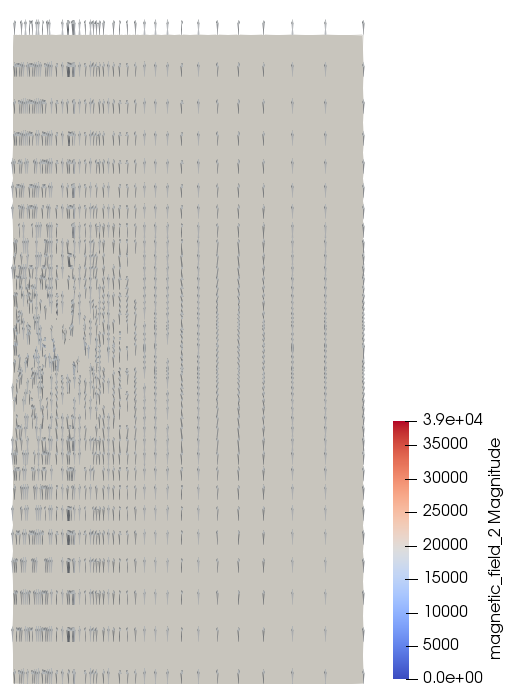
\includegraphics[width=0.95\textwidth]{magnetic_field_25.png}
\caption{Load step 25}
\label{fig:3.7.1}
\end{subfigure}
\begin{subfigure}{0.32\textwidth}
\centering
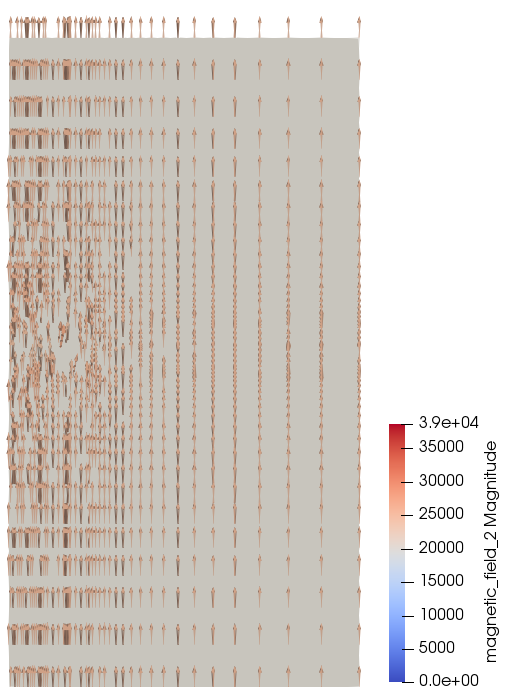
\includegraphics[width=0.95\textwidth]{magnetic_field_35.png}
\caption{Load step 35}
\label{fig:3.7.2}
\end{subfigure}
\begin{subfigure}{0.32\textwidth}
\centering
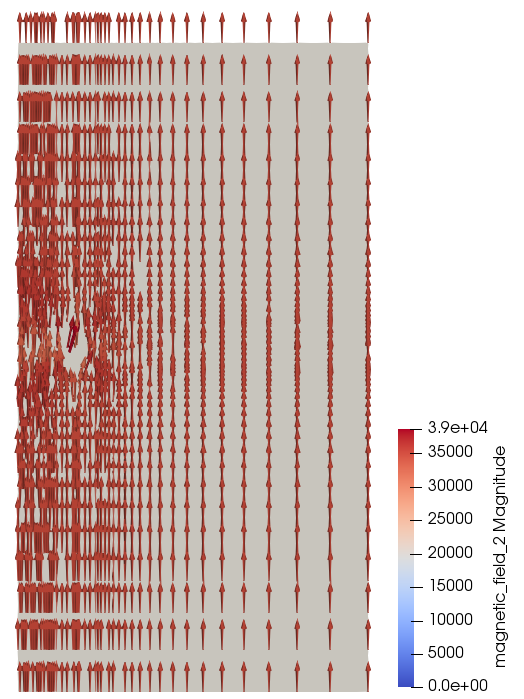
\includegraphics[width=0.95\textwidth]{magnetic_field_50.png}
\caption{Load step 50 (Half load)}
\label{fig:3.7.3}
\end{subfigure}
\caption{Magnetic field $\mathbb{H}$ increasing with each load step in first half of the total load application cycle}
\label{fig:3.7}
\end{figure}

The resulting magnetic field is observed in \Crefrange{fig:3.7.1}{fig:3.7.3}. As already stated, we observe the quadratic convergence of Newton solver only in close vicinity to the solution. The main advantage of the approach of linearly increasing the applied magnetic potential in small increments is that for each small increment the non-linear Newton solver would converge to a solution. Whereas if one were to apply such a large magnetic load in a single load step, we would observe no convergence and no solution corresponding to this large load value. \par 

\section{Variational formulation}

The corresponding system of partial differential equations (the strong forms of the local balance equations) for each field, the scalar-valued magnetic potential field in Task 1 and the vector-valued displacement field for an axisymmetric solid in Task 2.1, were described in details. The required boundary conditions to formulate a boundary-value problem were also mentioned for both the individual field (decoupled) problems. We now consider the fully-coupled problem of the (axisymmetric) magneto-elastic membrane immersed in a free space. The strong form of the complete system for the coupled problem in the total Lagrangian formulation is as follows:
\begin{align}
\text{Kinematics}:& \ \mathbb{H}, \ \mathbf{F}, \ \mathbf{C} := \mathbf{F}^T \cdot \mathbf{F}, \ \mathbf{E} := \dfrac{1}{2} (\mathbf{C} - \mathbf{I}) \label{eq:3.22.1}\\
\text{Equilibrium}:& \ \text{Div} \mathbb{B} = 0 \label{eq:3.22.2}\\
& \ \text{Div}(\mathbf{F} \cdot \mathbf{S}) + \mathbf{b}^p = \mathbf{0} \label{eq:3.22.3}\\
\text{Constitutive equation}:& \ \mathbb{B} = -\dfrac{\partial \Psi (J, \mathbf{C}, \mathbb{H})}{\partial \mathbb{H}} \label{eq:3.22.4}\\
& \ \mathbf{S} = 2\dfrac{\partial \Psi (J, \mathbf{C}, \mathbb{H})}{\partial \mathbf{C}}.
\label{eq:3.22.5}
\end{align}
The boundary conditions to be enforced for each field are: 
\begin{align}
\mathbf{N} \cdot \llbracket \mathbb{B} \rrbracket = 0 \ \text{on} \ \partial \mathcal{S}_{0, \phi}, \label{eq:3.23.1}\\
\mathbf{u} = \mathbf{u}^p \ \text{on} \ \partial \mathcal{S}_{0, \mathbf{u}}, \label{eq:3.23.2}\\
\mathbf{F} \cdot \mathbf{S} \cdot \mathbf{N} = \mathbf{t}^p \ \text{on} \ \partial \mathcal{B}_{0, t}.
\label{eq:3.23.3}
\end{align}
\Cref{eq:3.23.1} at the bounding surface of the free space material enforces the normal component of the referential magnetic induction vector field to remain continuous on the specified boundary \cite{pelteret2016}. This is a natural boundary condition in the unreformed configuration. \Cref{eq:3.23.2} is the homogeneous Dirichlet boundary condition for the displacement field. Here, the displacements on the free space boundary are constrained to zero. \Cref{eq:3.23.3} is the traction on the inner interface of the circular cross-section torus magneto-elastic membrane. From a mechanical perspective, this constitutes to a quasi-static inflating pressure load on the membrane and is analogues to an effect such as the air blown in a toy balloon to inflate the balloon. \newline \par 

\noindent \textbf{Principle of stationary potential energy:} \\
Based on the S.E.F. \Cref{eq:3.5}, to derive the weak form of the governing equations, we define the total potential energy function as
\begin{align}
\Pi &= \Pi_{int} + \Pi_{ext}, \\
\text{with} \ \Pi_{int} &= \int\limits_{\mathcal{D}_0} \Psi (J, \mathbf{C}, \mathbb{H}) \ \mathrm{d}V = \int\limits_{\mathcal{B}_0} \Psi_0^{\text{elas}} (\mathbf{C}) + \mu_r \int\limits_{\mathcal{B}_0} M_0 (J, \mathbf{C}, \mathbb{H}) + \int\limits_{\mathcal{S}_0} M_0 (J, \mathbf{C}, \mathbb{H}), \label{eq:3.24.1}\\
\text{and} \ \Pi_{ext} &= -\int\limits_{\mathcal{B}_0} \mathbf{u} \cdot \mathbf{b}^p \mathrm{d} V - \int\limits_{\partial \mathcal{B}_{0,t}} \mathbf{u} \cdot \mathbf{t}^p \mathrm{d}A -\int\limits_{\partial \mathcal{S}_{0,\mathbb{B}}} \phi \left[ \mathbb{B}_{\infty} \cdot \mathbf{N}_{\infty} \right] \mathrm{d}A.  
\label{eq:3.24.2}
\end{align}
The internal energy contribution \Cref{eq:3.24.1} is a sum of total potential energy per unit volume due to magneto-elastic material's deformation and magnetisation and the magnetic energy stored in the free space. The external energy contribution \Cref{eq:3.24.2} accounts for the referential mechanical body and traction forces respectively, and the last term describes the magnetic induction prescribed on the far-field boundary of the free space material. Due to the assumption that the magnetic field and magnetic induction are co-aligned, the last term in $\Pi_{ext}$ drops out. \par 

The stationary (saddle-)point $\min_{\mathbf{u}} \max_{\phi} \Pi \implies \delta \Pi$ describes the equilibrium solution to the coupled boundary value problem. The stationary point $\min_{\mathbf{u}} \max_{\phi} \Pi$ is that point at which all the directional derivatives of the total potential energy vanish. Using the G\^ateaux derivative we have
\begin{align}
\delta \Pi &= D_{\delta \mathbf{u}} \Pi_{int} + D_{\delta \phi} \Pi_{int} + D_{\delta \mathbf{u}} \Pi_{ext} + D_{\delta \phi} \Pi_{ext} = 0, \label{eq:3.25} \\
&= \delta \Pi_{int} + \delta \Pi_{ext}. \nonumber
\end{align}
The components of the variation of the internal potential energy are given as \cite{Saxena2015}
\begin{align}
D_{\delta \mathbf{u}} \Pi_{int} &= \int\limits_{\mathcal{D}_0} \delta \mathbf{E} : \mathbf{S} \ \mathrm{d}V, \label{eq:3.26.1}\\
D_{\delta \phi} \Pi_{int} &= -\int\limits_{\mathcal{D}_0} \delta \mathbb{H} \cdot \mathbb{B} \ \mathrm{d}V,
\label{eq:3.26.2}
\end{align}
and that of the external potential energy are
\begin{align}
D_{\delta \mathbf{u}} \Pi_{ext} &= -\int\limits_{\mathcal{B}_0} \delta \mathbf{u} \cdot \mathbf{b}^p \mathrm{d}V - \int\limits_{\partial \mathcal{B}_{0,t}} \delta \mathbf{u} \cdot \mathbf{t}^p \mathrm{d}A, \label{eq:3.27.1}\\
D_{\delta \phi} \Pi_{ext} &= 0.
\label{eq:3.27.2}
\end{align}
The variations of the kinematic quantities are defined as 
\begin{align}
\delta \mathbf{F} &= \nabla_0 \delta \mathbf{u}, \\
\delta \mathbf{E} &= \left[ \mathbf{F}^T \cdot \delta \mathbf{F} \right]^{\text{sym}}, \\ 
\delta \mathbb{H} &= -\nabla_0 \delta \phi \ \ \text{ from \Cref{eq:3.0}}.
\label{eq:3.28}
\end{align}
The second Piola-Kirchhoff stress $\mathbf{S}$ in \Cref{eq:3.26.1} can further be split into two components, the total stress within the elastic body (membrane) and the Maxwell stress contribution from the free space (non-magnetisable) material respectively, as follows:
\begin{align}
\mathbf{S} &= \mathbf{S}^{\text{tot}} + \mathbf{S}^{\text{max}} =: 2 \dfrac{\partial \Psi (J, \mathbf{C}, \mathbb{H})}{\partial \mathbf{C}}, \\
\text{with} \ \mathbf{S}^{\text{tot}} &= 2 \dfrac{\partial \Psi_0^{\text{elas}} (\mathbf{C})}{\partial \mathbf{C}} + 2 \mu_r \dfrac{M_0 (J, \mathbf{C}, \mathbb{H})}{\partial \mathbf{C}}, \ \ (\text{note:} \ \mu_r > 1)\\
\text{and} \ \mathbf{S}^{\text{max}} &= 2 \dfrac{M_0 (J, \mathbf{C}, \mathbb{H})}{\partial \mathbf{C}}  \ \ (\text{note:} \ \mu_r = 1).
\end{align}
Similarly, the referential magnetic induction vector $\mathbb{B}$ in \Cref{eq:3.26.2} can be split into the induction within the elastic solid and the induction in the free space material as
\begin{align}
\mathbb{B} &= \mathbb{B}^{\text{tot}} + \mathbb{B}^{\text{max}} =: -\dfrac{\partial \Psi (J, \mathbf{C}, \mathbb{H})}{\partial \mathbb{H}}, \\
\text{with} \ \mathbb{B}^{\text{tot}} &= -\dfrac{\partial \Psi_0^{\text{elas}} (\mathbf{C})}{\partial \mathbb{H}} - \mu_r \dfrac{M_0 (J, \mathbf{C}, \mathbb{H})}{\partial \mathbb{H}}, \ \ (\text{note:} \ \mu_r > 1)\\
\text{and} \ \mathbb{B}^{\text{max}} &= -\dfrac{M_0 (J, \mathbf{C}, \mathbb{H})}{\partial \mathbb{H}}, \ \ (\text{note:} \ \mu_r = 1).
\end{align}
\Crefrange{eq:3.25}{eq:3.27.2} collectively represent the equivalent weak form of the equilibrium equations of our interest as mentioned in \Cref{eq:3.22.2,eq:3.22.3}. The continuity of the normal magnetic induction as given in \Cref{eq:3.23.1} at the material interfaces is also satisfied within this formulation. \par 

\noindent The variations in \Cref{eq:3.26.2,eq:3.27.1} belong to the following space
\begin{equation}
\delta \mathbf{u} \in H^1 (\overline{\mathcal{B}_0}), \ \ \delta \phi \in H^1 (\overline{\mathcal{B}_0}, \cup \ \mathcal{S}_0),
\end{equation}
with the constraints 
\begin{equation}
\delta \mathbf{u} = \mathbf{0} \ \text{on} \ \partial \mathcal{B}_{0,\mathbf{u}} \cup \left[ \overline{\mathcal{S}_0} \setminus \Gamma_{0, \mathcal{BS}} \right], \ \ \delta \phi = 0 \ \text{on} \ \partial \mathcal{B}_{0,\phi} \ \text{and} \ \partial \mathcal{S}_{0,\phi},
\end{equation}
where $\Gamma_{0, \mathcal{BS}} = \overline{\mathcal{S}_0} \cap \overline{\mathcal{B}_0}$ indicates the boundary of the magneto-elastic solid body exposed to the free space material. As the employed material law for the magneto-elastic material is non-linear Neo-Hookean, the linearisation of \Cref{eq:3.26.1,eq:3.26.2} ($\delta \Pi_{int}$) is required within an iterative solution scheme such as the Newton-Raphson method to find the stationary point of the saddle-point system. 

\section{Linearisation of the coupled problem}
Assuming the state of the system is known at some load or time step $t_{n-1}$, the linearisation by employing the first-order Taylor expansion of the variation of total potential energy is given as: Find $\Delta \mathbf{u}$ and $\Delta \phi$ such that
\begin{equation}
\mathbf{L} \left[ \delta \Pi \right]_{\phi_{i+1}, \mathbf{u}_{i+1}} = \delta \Pi \Big{|}_{\phi_i, \mathbf{u}_i} + D_{\Delta \phi} \Big[ D_{\delta \phi} \Pi_{int} + D_{\delta \mathbf{u}} \Pi_{int} \Big] + D_{\Delta \mathbf{u}} \Big[ D_{\delta \phi} \Pi_{int} + D_{\delta \mathbf{u}} \Pi_{int} \Big],
\label{eq:3.29}
\end{equation} 
where $\Delta \left\lbrace \cdot \right\rbrace := \left\lbrace \cdot \right\rbrace_{i+1} - \left\lbrace \cdot \right\rbrace_i$ is the incremental change between the iterative solver iterations $i$ and $i+1$ and the value of a quantity at the current Newton iteration at the currently unknown load/time state $t_n$ is denoted as $\left\lbrace \cdot \right\rbrace_i^n = \left\lbrace \cdot \right\rbrace_i$.

Assuming dead load ($\mathbf{b}^p = \mathbf{0}$), the direct terms of linearisation are given as:
\begin{align}
D^2_{\Delta \phi, \delta \phi} \Pi_{int} &= - \int\limits_{\mathcal{D}_0} \delta \mathbb{H} \cdot \mathbf{D} \cdot \Delta \mathbb{H} \ \mathrm{d}V, \label{eq:3.30.1}\\
D^2_{\Delta \mathbf{u}, \delta \mathbf{u}} \Pi_{int} &= \int\limits_{\mathcal{D}_0} \Delta \delta \mathbf{E} : \mathbf{S} \ \mathrm{d}V + \int\limits_{\mathcal{D}_0} \delta \mathbf{E} : \mathfrak{C} : \Delta \mathbf{E} \ \mathrm{d}V, \label{eq:3.30.2}
\end{align}
where $\Delta \delta \mathbf{E} = \left[ \Delta \mathbf{F}^T \cdot \delta \mathbf{F} \right]^{\text{sym}}, \ \mathbf{D} := \dfrac{\partial \mathbb{B}}{\partial \mathbb{H}} = -\dfrac{\partial^2 \Psi (J, \mathbf{C}, \mathbb{H})}{\partial \mathbb{H} \otimes \partial \mathbb{H}}$ is the rank-2 magneto-static tensor and $\mathfrak{C} := 2\dfrac{\partial \mathbf{S}}{\partial \mathbf{C}} = 4\dfrac{\partial^2 \Psi (J, \mathbf{C}, \mathbb{H})}{\partial \mathbf{C} \otimes \partial \mathbf{C}}$ is the referential elastic tangent as derived earlier in \Cref{eq:3.9}. The detailed linearisation of the kinematical quantity $\mathbf{E}$, i.e. the Green-Lagrange strain tensor, and the constitutive equation $\mathbf{S}$, the second Piola-Kirchhoff stress tensor is already discussed in Task 2.1 and the same result applies here. \par 

The coupled terms arising from the linearisation are
\begin{align}
D^2_{\Delta \phi, \delta \mathbf{u}} \Pi_{int} &= - \int\limits_{\mathcal{D}_0} \delta \mathbf{E} : \mathbb{P} \cdot \Delta \mathbb{H} \ \mathrm{d}V, \label{eq:3.31.1} \\
D^2_{\Delta \mathbf{u}, \delta \phi} \Pi_{int} &= - \int\limits_{\mathcal{D}_0} \delta \mathbb{H} \cdot \mathbb{P}^T : \Delta \mathbf{E} \ \mathrm{d}V, \label{eq:3.31.2}
\end{align}
where $\mathbb{P} := -\dfrac{\partial \mathbf{S}}{\partial \mathbb{H}} = -2 \dfrac{\partial^2 \Psi (J, \mathbf{C}, \mathbb{H})}{\partial \mathbf{C} \otimes \mathbb{H}}$ and $\mathbb{P}^T := 2 \dfrac{\partial \mathbb{B}}{\partial \mathbf{C}} = -2 \dfrac{\partial^2 \Psi (J, \mathbf{C}, \mathbb{H})}{\partial \mathbb{H} \otimes \partial \mathbf{C}}$ are the referential magneto-elasticity tensors. \par 

The final linear form of \Cref{eq:3.25} can be written as:
\begin{align}
D_{\delta \phi} \Pi + D^2_{\Delta \phi, \delta \phi} \Pi + D^2_{\Delta \phi, \delta \mathbf{u}} \Pi = \mathbf{0}, \nonumber \\
D_{\delta \mathbf{u}} \Pi + D^2_{\Delta \mathbf{u}, \delta \mathbf{u}} \Pi + D^2_{\Delta \mathbf{u}, \delta \phi} \Pi = \mathbf{0}.
\label{eq:3.35}
\end{align}
 
The derived forms for the terms $\mathbf{D}$ and $\mathbb{P}$ will be presented below. To derive $\mathbf{D}$, we first need to derive the referential magnetic induction vector as follows:
\begin{align*}
\mathbb{B} &= - \dfrac{\partial \Psi (J, \mathbf{C}, \mathbb{H})}{\partial \mathbb{H}} = - \dfrac{\partial M_0 (J, \mathbf{C}, \mathbb{H})}{\partial \mathbb{H}}\\
&= \dfrac{\mu_0 \mu_r}{2} \dfrac{\partial [J \ \mathbf{C}^{-1} : \mathbb{H} \otimes \mathbb{H}]}{\partial \mathbb{H}} \\
&= \dfrac{\mu_0 \mu_r}{2} \dfrac{\partial [J \ C^{-1}_{IJ} \ H_I \ H_J	]}{\partial H_K} \mathbf{E}_K \\
&= \dfrac{\mu_0 \mu_r}{2} \left[ J \ C^{-1}_{IJ} \dfrac{\partial H_I}{\partial H_K} \ H_J + J \ C^{-1}_{IJ} \ H_I \dfrac{\partial H_J}{\partial H_K} \right] \mathbf{E}_K \\
&= \dfrac{\mu_0 \mu_r}{2} \left[ J \ C^{-1}_{IJ} \ \delta_{IK} \ H_J + J \ C^{-1}_{IJ} \ H_I \ \delta_{JK} \right] \mathbf{E}_K \\
&= \dfrac{\mu_0 \mu_r}{2} J \left[ \ C^{-1}_{JI} \ \delta_{IK} \ H_J + \ C^{-1}_{IJ} \ \delta_{JK} \ H_I \right] \mathbf{E}_K \\
&= \dfrac{\mu_0 \mu_r}{2} J \left[ \ C^{-1}_{JK} \ H_J + \ C^{-1}_{IK} \ H_I \right] \mathbf{E}_K \\
&= \dfrac{\mu_0 \mu_r}{2} J \left[ \ C^{-1}_{KJ} \ H_J + \ C^{-1}_{KI} \ H_I \right] \mathbf{E}_K
\end{align*}
\begin{empheq}[box=\tcbhighmath]{align}
\mathbb{B} = \mu_0 \mu_r \ J \ [\mathbf{C}^{-1} \cdot \mathbb{H}].
\label{eq:3.32}
\end{empheq}

The derivation for the rank-2 magnetic tensor $\mathbf{D}$ is as follows:
\begin{align*}
\mathbf{D} &= \dfrac{\partial \mathbb{B}}{\partial \mathbb{H}} \\
&= \dfrac{\partial [\mu_0 \mu_r \ J \ (\mathbf{C}^{-1} \cdot \mathbb{H})]}{\partial \mathbb{H}} \\
&= \mu_0 \mu_r \ J \ \dfrac{\partial (C^{-1}_{IJ} \ H_J)}{\partial H_K} \ \mathbf{E}_I \otimes \mathbf{E}_K \\
&= \mu_0 \mu_r \ J \ C^{-1}_{IJ} \ \dfrac{\partial H_J}{\partial H_K} \ \mathbf{E}_I \otimes \mathbf{E}_K \\
&= \mu_0 \mu_r \ J \ C^{-1}_{IJ} \ \delta_{JK} \ \mathbf{E}_I \otimes \mathbf{E}_K \\
&= \mu_0 \mu_r \ J \ C^{-1}_{IK} \ \mathbf{E}_I \otimes \mathbf{E}_K
\end{align*}
\begin{empheq}[box=\tcbhighmath]{align}
\mathbf{D} &= \mu_0 \mu_r \ J \ \mathbf{C}^{-1}.
\label{eq:3.33}
\end{empheq}

The magneto-elasticity tensor quantity $\mathbb{P}$ defines the sensitivity of the second Piola-Kirchhoff stress $\mathbf{S}$ w.r.t. the applied referential magnetic field $\mathbb{H}$ and can be derived as follows:
\begin{align*}
\mathbb{P} &= -\dfrac{\partial \mathbf{S}}{\partial \mathbb{H}} = -\dfrac{\partial}{\partial \mathbb{H}} \left( 2 \dfrac{\partial \Psi (J, \mathbf{C}, \mathbb{H})}{\partial \mathbf{C}} \right) = -2 \ \dfrac{\partial^2 \Psi (J, \mathbf{C}, \mathbb{H})}{\partial \mathbf{C} \otimes \partial \mathbb{H}}\\
\intertext{Employing the result of \Cref{eq:3.6} for $\mathbf{S}$, we have}
&= \dfrac{\mu_0 \mu_r}{2} \ J \ \left[ \mathbf{C}^{-1} \otimes \dfrac{\partial}{\partial \mathbb{H}} \left( \mathbf{C}^{-1} : \mathbb{H} \otimes \mathbb{H} \right) \right] - \mu_0 \mu_r \ J \ \dfrac{\partial [ (\mathbf{C}^{-1} \cdot \mathbb{H}) \otimes (\mathbf{C}^{-1} \cdot \mathbb{H}) ]^{sym}}{\partial \mathbb{H}}
\end{align*}
Side calculation 1:
\begin{align*}
\dfrac{\partial \left( \mathbf{C}^{-1} : \mathbb{H} \otimes \mathbb{H} \right)}{\partial \mathbb{H}} &= \dfrac{\partial \left( C^{-1}_{IJ} \ H_I \ H_J \right)}{\partial H_K} \mathbf{E}_K \\
&= \left[ C^{-1}_{IJ} \ \delta_{IK} \ H_J + C^{-1}_{IJ} \ H_I \ \delta_{JK} \right] \ \mathbf{E}_K \\
&= \left[ C^{-1}_{JI} \ \delta_{IK} \ H_J + C^{-1}_{IJ} \ \delta_{JK} \ H_I \right] \ \mathbf{E}_K \\
&= \left[ C^{-1}_{JK} \ H_J + C^{-1}_{IK} \ H_I \right] \ \mathbf{E}_K \\
&= \left[ C^{-1}_{KJ} \ H_J + C^{-1}_{KI} \ H_I \right] \ \mathbf{E}_K \\
&= 2 [\mathbf{C}^{-1} \cdot \mathbb{H}]
\end{align*}
Side calculation 2:
\begin{align*}
\dfrac{\partial [ (\mathbf{C}^{-1} \cdot \mathbb{H}) \otimes (\mathbf{C}^{-1} \cdot \mathbb{H}) ]^{sym}}{\partial \mathbb{H}} &= \dfrac{1}{2} \dfrac{\partial \left[ C^{-1}_{IM} \ H_M \ C^{-1}_{JN} \ H_N + C^{-1}_{JM} \ H_M \ C^{-1}_{IN} \ H_N \right]}{\partial H_K} \ \mathbf{E}_I \otimes \mathbf{E}_J \otimes \mathbf{E}_K \\
\begin{split}
= & \ \dfrac{1}{2} \left[ C^{-1}_{IM} \ \delta_{MK} \ C^{-1}_{JN} \ H_N + C^{-1}_{IM} \ H_M \ C^{-1}_{JN} \ \delta_{NK} \right] \ \mathbf{E}_I \otimes \mathbf{E}_J \otimes \mathbf{E}_K  \\
&+ \dfrac{1}{2} \left[ C^{-1}_{JM} \ \delta_{MK} \ C^{-1}_{IN} \ H_N + C^{-1}_{JM} \ H_M \ C^{-1}_{IN} \ \delta_{NK} \right] \ \mathbf{E}_I \otimes \mathbf{E}_J \otimes \mathbf{E}_K \\
\end{split}\\
\begin{split}
= & \ \dfrac{1}{2} \left[ C^{-1}_{IK} \ C^{-1}_{JN} \ H_N + C^{-1}_{IM} \ H_M \ C^{-1}_{JK} \right] \ \mathbf{E}_I \otimes \mathbf{E}_J \otimes \mathbf{E}_K \\
&+ \dfrac{1}{2} \left[ C^{-1}_{JK} \ C^{-1}_{IN} \ H_N + C^{-1}_{JM} \ H_M \ C^{-1}_{IK} \right] \ \mathbf{E}_I \otimes \mathbf{E}_J \otimes \mathbf{E}_K \\
\end{split}\\
\intertext{Observing the symmetry over the indices $I$ and $J$, we have}
&= \left[ C^{-1}_{IK} \ C^{-1}_{JN} \ H_N + C^{-1}_{IM} \ H_M \ C^{-1}_{JK} \right] \ \mathbf{E}_I \otimes \mathbf{E}_J \otimes \mathbf{E}_K \\
&= \mathbf{C}^{-1} \otimes (\mathbf{C}^{-1} \cdot \mathbb{H}) + (\mathbf{C}^{-1} \cdot \mathbb{H}) \otimes \mathbf{C}^{-1}
\end{align*}
\begin{empheq}[box=\tcbhighmath]{align}
\mathbb{P} &= \mu_0 \mu_r \ J \ \left[  \mathbf{C}^{-1} \otimes (\mathbf{C}^{-1} \cdot \mathbb{H}) \right] -  \mu_0 \mu_r \ J \ \left[ \mathbf{C}^{-1} \otimes (\mathbf{C}^{-1} \cdot \mathbb{H}) + (\mathbf{C}^{-1} \cdot \mathbb{H}) \otimes \mathbf{C}^{-1} \right].
\label{eq:3.34}
\end{empheq}


\section{Discretization by the finite element method}
We now discretize the variational form \Cref{eq:3.35} by introducing the standard Lagrangian finite element basis for the scalar-valued magnetic potential $\phi$ and the vector-valued displacement $\mathbf{u}$ as
\begin{align}
\phi (\mathbf{X}) &\approx \phi^h (\mathbf{X}) = \sum\limits_{I} \phi_I N_I (\mathbf{X}), \ \ \ \ \mathbf{u} (\mathbf{X}) \approx \mathbf{u}^h (\mathbf{X}) = \sum\limits_{I} u_I \mathbf{N}_I (\mathbf{X}), \\
\nabla_0 \phi (\mathbf{X}) &\approx \nabla_0 \phi^h (\mathbf{X}) = \sum\limits_{I} \phi_I \nabla_0 N_I (\mathbf{X}), \ \ \nabla_0 \mathbf{u} (\mathbf{X}) \approx \nabla_0 \mathbf{u}^h (\mathbf{X}) = \sum\limits_{I} u_I \nabla_0 \mathbf{N}_I (\mathbf{X}),
\end{align}
with $\phi_I \in \mathbb{R}$ and $u_I \in \mathbb{R}$. $N_I$ and $\mathbf{N}_I$ are, respectively, the scalar-valued and vector-valued shape functions corresponding to the global degree of freedom (support point) $I$. Let the collective solution vector be called as $\mathbf{d} = \left\lbrace \phi; \mathbf{u} \right\rbrace^T$. The shape functions belong to the Sobolev space which is defined as
\begin{equation}
H^1 (\mathcal{D}_0; \mathbb{R}^{\text{dim}}) = \left\lbrace \mathbf{d} : \mathcal{D}_0 \mapsto \mathbb{R} \Big{|} \int\limits_{\mathcal{D}_0} \norm{\mathbf{d}}^2 + \norm{\nabla \mathbf{d}}^2 \ \mathrm{d}\mathcal{D}_0 < \infty \right\rbrace.
\end{equation}
The discrete function spaces for the solution fields are given as
\begin{align}
S^h &= \left\lbrace \phi^h \in H^1, \ \phi^h|_{\partial \mathcal{S}_{0, \phi}} = \overline{\phi^h} \right\rbrace, \\
\mathbf{W}^h &= \left\lbrace \mathbf{u}^h \in H^1, \ \mathbf{u}^h|_{\partial \mathcal{B}_{0, \mathbf{u}} \cup \partial \mathcal{S}_{0, \mathbf{u}}} = \overline{\mathbf{u}^h} \right\rbrace.
\end{align}

\noindent The variations and linearization of the discretized fields are given as
\begin{align}
\delta \phi^h (\mathbf{X}) &= \sum\limits_{I} \delta \phi_I N_I (\mathbf{X}), \ \ \ \ \delta  \mathbf{u}^h (\mathbf{X}) = \sum\limits_{I} \delta u_I \mathbf{N}_I (\mathbf{X}), \\
\Delta \phi^h (\mathbf{X}) &= \sum\limits_{I} \Delta \phi_I N_I (\mathbf{X}), \ \ \Delta \mathbf{u}^h (\mathbf{X}) = \sum\limits_{I} \Delta u_I \mathbf{N}_I (\mathbf{X}),
\end{align}
with $\delta \phi_I, \Delta \phi_I \in \mathbb{R}$ and $\delta u_I, \Delta u_I \in \mathbb{R}$. \par 

\noindent The discrete function spaces for the variation of the solution fields are given as
\begin{align}
T^h &= \left\lbrace \delta\phi^h \in H^1, \ \delta\phi^h|_{\partial \mathcal{S}_{0, \phi}} = 0 \right\rbrace, \\
\mathbf{V}^h &= \left\lbrace \delta\mathbf{u}^h \in H^1, \ \delta\mathbf{u}^h|_{\partial \mathcal{B}_{0, \mathbf{u}} \cup \partial \mathcal{S}_{0, \mathbf{u}}} = \mathbf{0} \right\rbrace.
\end{align}

\noindent The derivatives of the increments of the solution fields are given as
\begin{align}
\nabla_0 \Delta \phi^h (\mathbf{X}) &= \sum\limits_{I} \Delta \phi_I \nabla_0 N_I (\mathbf{X}), \ \ \nabla_0 \Delta \mathbf{u}^h (\mathbf{X}) = \sum\limits_{I} \Delta u_I \nabla_0 \mathbf{N}_I (\mathbf{X}).
\end{align} \newline

The resulting discretized system of equations for the final linearised variational form \Cref{eq:3.35} employing the results from \Crefrange{eq:3.26.1}{eq:3.27.2}, \Crefrange{eq:3.30.1}{eq:3.31.2} and the definitions for the variations \Cref{eq:3.28} can be written in the form of the following L.H.S. and R.H.S.:
\begin{align}
\text{L.H.S.:} \ = &- \sum\limits_I \sum\limits_J \delta \phi_I \int\limits_{\mathcal{D}_0} \left[ \nabla_0 N_I (\mathbf{X}) \cdot \mathbf{D} \cdot \nabla_0 N_J (\mathbf{X}) \right] \cdot \Delta \phi_J \ \mathrm{d}V \nonumber \\
&+ \sum\limits_I \sum\limits_J \delta u_I \int\limits_{\mathcal{D}_0} \left[ \left[ \mathbf{F}^T \cdot \nabla_0 \mathbf{N}_I (\mathbf{X}) \right] : \mathbb{P} \cdot \nabla_0 N_J (\mathbf{X}) \right] \cdot \Delta \phi_J \ \mathrm{d}V \nonumber \\
&+ \sum\limits_I \sum\limits_J \delta \phi_I \int\limits_{\mathcal{D}_0} \left[ \nabla_0 N_I (\mathbf{X}) \cdot \mathbb{P}^T : \left[ \mathbf{F}^T \cdot \nabla_0 \mathbf{N}_J (\mathbf{X}) \right] \right] \cdot \Delta u_J \ \mathrm{d}V \nonumber \\
&+ \sum\limits_I \sum\limits_J \delta u_I \int\limits_{\mathcal{D}_0} \left[ \left[ \nabla_0 \mathbf{N}_I^T (\mathbf{X}) \cdot \nabla_0 \mathbf{N}_J (\mathbf{X}) \right]^{\text{sym}} : \mathbf{S} \right] \cdot \Delta u_J \ \mathrm{d}V \nonumber \\
&+ \sum\limits_I \sum\limits_J \delta u_I \int\limits_{\mathcal{D}_0} \left[ \left[ \mathbf{F}^T \cdot \nabla_0 \mathbf{N}_I (\mathbf{X}) \right]^{\text{sym}} : \mathfrak{C} : \left[ \mathbf{F}^T \cdot \nabla_0 \mathbf{N}_J (\mathbf{X}) \right]^{\text{sym}} \right] \cdot \Delta u_J \ \mathrm{d}V.
\label{eq:3.36}
\end{align}
\begin{align}
\text{R.H.S.:} \ = &- \sum\limits_I \delta u_I \int\limits_{\mathcal{D}_0} \left[ \left[ \mathbf{F}^T \cdot \nabla_0 \mathbf{N}_I (\mathbf{X}) \right]^{\text{sym}} : \mathbf{S} \right] \ \mathrm{d}V \nonumber \\
&- \sum\limits_I \delta \phi_I \int\limits_{\mathcal{D}_0} \left[ \nabla_0 N_I (\mathbf{X}) \cdot \mathbb{B} \right] \ \mathrm{d}V \nonumber \\
&+ \sum\limits_I \delta u_I \int\limits_{\partial \mathcal{B}_{0,t}} \left[ \mathbf{N}_I (\mathbf{X}) \cdot \mathbf{t}^p \right] \ \mathrm{d}A.
\label{eq:3.37}
\end{align}
The resulting discretized equations \Cref{eq:3.36,eq:3.37} must hold for all arbitrary variations $\delta \phi_I$ and $\delta u_I$. The algebraic system to be solved at time/load step $t_n$ and Newton iterate $i$ is
\begin{equation}
\begin{bmatrix}
\mathbf{K}_{\phi \phi} & \mathbf{K}_{\phi \mathbf{u}} \\
\mathbf{K}_{\mathbf{u} \phi} & \mathbf{K}_{\mathbf{u} \mathbf{u}}
\end{bmatrix}
\begin{bmatrix}
\Delta \mathbf{d}_{\phi} \\
\Delta \mathbf{d}_{\mathbf{u}}
\end{bmatrix}
=
\begin{bmatrix}
-\mathbf{R}_{\phi} \\
-\mathbf{R}_{\mathbf{u}}
\end{bmatrix}
\implies \ \mathbf{K} \cdot \Delta \mathbf{d} = -\mathbf{R}.
\label{eq:3.10}
\end{equation}
The solution update is then performed as follows
\begin{equation}
\mathbf{d}_{i+1}^n = \mathbf{d}_i^n + \Delta \mathbf{d}^n.
\label{eq:3.38}
\end{equation}
Applying the Gauss quadrature rule for the numerical integration and also considering the transformation needed for the axisymmetric formulation (as previously discussed in Task 1 and 2.1), the final cell wise FE assembly is given as follows:
\begin{align}
K_{IJ} = &- \sum\limits_q \left[ \nabla_0 N_I (q) \cdot \mathbf{D} \cdot \nabla_0 N_J (q) \right] \ C.S.F. \ J \ w(q) \nonumber \\
&+ \sum\limits_q \left[ \left[ \mathbf{F}^T \cdot \nabla_0 \mathbf{N}_I (q) \right] : \mathbb{P} \cdot \nabla_0 N_J (q) \right] \ C.S.F. \ J \ w(q) \nonumber \\
&+ \sum\limits_q \left[ \nabla_0 N_I (q) \cdot \mathbb{P}^T : \left[ \mathbf{F}^T \cdot \nabla_0 \mathbf{N}_J (q) \right] \right] \ C.S.F. \ J \ w(q) \nonumber \\
&+ \sum\limits_q \left[ \left[ \nabla_0 \mathbf{N}_I^T (q) \cdot \nabla_0 \mathbf{N}_J (q) \right]^{\text{sym}} : \mathbf{S} \right]  \ C.S.F. \ J \ w(q) \nonumber \\
&+ \sum\limits_q \left[ \left[ \mathbf{F}^T \cdot \nabla_0 \mathbf{N}_I (q) \right]^{\text{sym}} : \mathfrak{C} : \left[ \mathbf{F}^T \cdot \nabla_0 \mathbf{N}_J (q) \right]^{\text{sym}} \right] \ C.S.F. \ J \ w(q),
\label{eq:3.39}
\end{align}
and with $\mathbf{f} := -\mathbf{R}$
\begin{align}
f_I = &- \sum\limits_q \left[ \left[ \mathbf{F}^T \cdot \nabla_0 \mathbf{N}_I (q) \right]^{\text{sym}} : \mathbf{S} \right] \ C.S.F. \ J \ w(q) \nonumber \\
&- \sum\limits_q \left[ \nabla_0 N_I (q) \cdot \mathbb{B} \right] \ C.S.F. \ J \ w(q) \nonumber \\
&+ \sum\limits_q \left[ \mathbf{N}_I (q) \cdot \mathbf{t}^p \right] \ C.S.F. \ J \ w(q),
\label{eq:3.40}
\end{align}
where $q$ are the local quadrature points with corresponding weights $w(q)$ and the scalar $C.S.F. := 2 \pi R$ is the co-ordinate scaling factor arising from the transformation of the 3D integrals to the axisymmetric (2.5D) integrals. $R$ is the axial component of the distance of the local quadrature point $q$ from the axis of symmetry. \Cref{eq:3.39,eq:3.40} represents the final FE assembly we have implemented for the axisymmetric fully-coupled magneto-elastic problem of our interest. \par 

\section{Implementation details}

\subsection{Saddle point system}

At any Newton iteration $i$ and time/load step $t_n$ the algebraic equations to solve are as represented in \Cref{eq:3.10}. Consider the scalar-valued magnetic potential solution block vector $\mathbf{d}_{\phi}$ be of size $p$ and the vector-valued displacement solution block vector $\mathbf{d}_{\mathbf{u}}$ for an axisymmetric formulation be of size $q$. Then the total number of unknowns, called as number of global DoFs, will be $n_{dofs} = p + q$. For the case where the same order finite elements are employed for both the fields, for e.g., for a total number of support points $n_d$, for linear Lagrange finite element $(Q_1)$ used for the solution field $\phi$ with $p = n_d$ and bi-linear Lagrange finite elements $(Q_1 \times Q_1)$ for the solution field $\mathbf{u}$ with $q = 2 n_d$, then the total number of unknowns would be $n_{dofs} = 3 n_d$. By definition, a support point is a point $p_i$ such that for a shape function $N_j$ (finite element families based on the Lagrange interpolation) it holds $N_j (p_i) = \delta_{ij}$. The corresponding tangent matrix blocks will be of the following dimensions:
\begin{equation}
\mathbf{K}_{\phi \phi} \in \mathbb{R}^{p \times p}, \ \mathbf{K}_{\phi \mathbf{u}} \in \mathbb{R}^{p \times q}, \ \mathbf{K}_{\mathbf{u} \phi} \in \mathbb{R}^{q \times p}, \ \mathbf{K}_{\mathbf{u} \mathbf{u}} \in \mathbb{R}^{q \times q}.
\end{equation}
The system of equations in \Cref{eq:3.10} represents a saddle point system for the coupled multi-physics problem of our interest. Saddle point systems arise when a certain quantity such as the energy of a continuum body has to be minimized, subject to a set of linear constraints. The constraints typically represent some basic conservation law such as the balance law of linear momentum in our case of non-linear solid mechanics. Because saddle point systems can be derived as equilibrium conditions for a physical system, they are sometimes also referred to a \textit{equilibrium equations} \cite{Benzi2005}. We therefore briefly discuss the saddle point systems and also mention the necessary requirements to be satisfied for a linear system of equations to be classified as a saddle point system. \newline \par 
For a general linear system 
\begin{equation}
\begin{bmatrix}
\mathbf{A} & \mathbf{B} \\
\mathbf{C} & \mathbf{D}
\end{bmatrix}
\begin{bmatrix}
\mathbf{x} \\
\mathbf{y}
\end{bmatrix}
=
\begin{bmatrix}
\mathbf{f} \\
\mathbf{g}
\end{bmatrix}
\implies \mathbf{K} \cdot \mathbf{u} = \mathbf{r}
\label{eq:3.11}
\end{equation}
equivalent to \Cref{eq:3.10} to be classified as a (generalized) saddle point problem, the individual blocks $\mathbf{A}, \mathbf{B}, \mathbf{C}, \mathbf{D}$ of the tangent matrix $\mathbf{K}$ have to satisfy one or more of the following conditions \cite{Benzi2005}:
\begin{itemize}
\item[C1] $\mathbf{A}$ is symmetric: $\mathbf{A} = \mathbf{A}^T$
\item[C2] Symmetric part of $\mathbf{A}$, $\mathbf{A}^{sym} = \dfrac{1}{2} \left( \mathbf{A} + \mathbf{A}^T \right)$, is positive semidefinite
\item[C3] $\mathbf{B} = \mathbf{C}$
\item[C4] $\mathbf{D}$ is symmetric and positive semidefinite
\item[C5] $\mathbf{D} = \mathbf{0}$ (zero matrix)
\end{itemize}
When all the above conditions are satisfied, the tangent matrix $\mathbf{K}$ is symmetric positive semidefinite and we have a symmetric linear system of equations. Consider the following minimization problem:
\begin{equation}
J(\mathbf{u}) = \dfrac{1}{2} \left\langle \mathbf{K} \cdot \mathbf{u}, \mathbf{u} \right\rangle - \left\langle \mathbf{r}, \mathbf{u} \right\rangle,
\label{eq:3.12}
\end{equation}
subject to 
\begin{equation}
\mathbf{C} \cdot \mathbf{x} = \mathbf{g},
\label{eq:3.13}
\end{equation}
with $\left\langle \cdot, \cdot \right\rangle$ denoting the standard inner product in $\mathbb{R}^{p+q}$.
Note that
\begin{equation}
\nabla J(\mathbf{u}) = \mathbf{K} \cdot \mathbf{u} - \mathbf{r}.
\end{equation}
Any solution $(\mathbf{x}_{\ast}, \mathbf{y}_{\ast})^T$ of the general case (satisfying all of the conditions C1-C5), is a saddle point of the Lagrangian defined as
\begin{equation}
\mathcal{L}(\mathbf{x}, \mathbf{y}) = \dfrac{1}{2} \left\langle \mathbf{K} \cdot \mathbf{u}, \mathbf{u} \right\rangle - \left\langle \mathbf{r}, \mathbf{u} \right\rangle + (\mathbf{C} \cdot \mathbf{x} - \mathbf{g})^T \cdot \mathbf{y}.
\label{eq:3.14}
\end{equation}
The saddle point $(\mathbf{x}_{\ast}, \mathbf{y}_{\ast})^T \in \mathbb{R}^{p+q}$ satisfies
\begin{equation}
\mathcal{L}(\mathbf{x}_{\ast}, \mathbf{y}) \leq \mathcal{L}(\mathbf{x}_{\ast}, \mathbf{y}_{\ast}) \leq \mathcal{L}(\mathbf{x}, \mathbf{y}_{\ast}) \ \forall \mathbf{x} \in \mathbb{R}^p \ \& \ \forall \mathbf{y} \in \mathbb{R}^q, 
\label{eq:3.15.1}
\end{equation}
or equivalently, 
\begin{equation}
\min_{\mathbf{x}} \max_{\mathbf{y}} \mathcal{L}(\mathbf{x}, \mathbf{y}) = \mathcal{L}(\mathbf{x}_{\ast}, \mathbf{y}_{\ast}) = \max_{\mathbf{x}} \min_{\mathbf{y}} \mathcal{L}(\mathbf{x}, \mathbf{y}).
\label{eq:3.15.2}
\end{equation}

\begin{figure}[h]
\centering
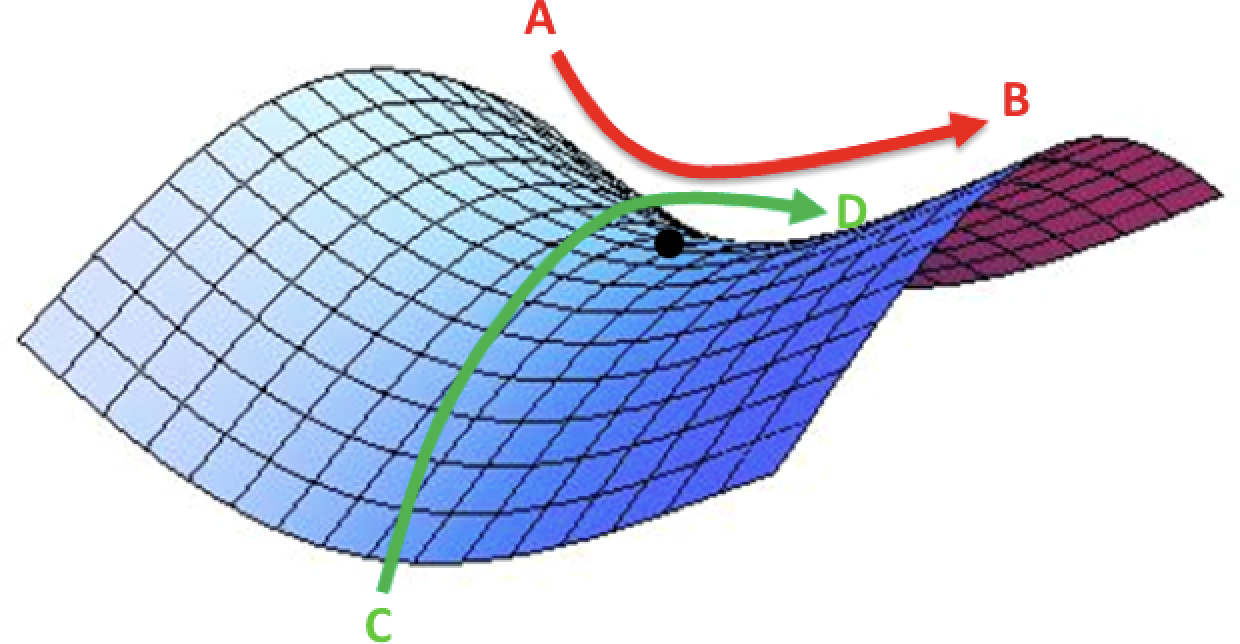
\includegraphics[width=0.6\textwidth]{saddle_point_problem.png}
\caption{Saddle point over a 3D surface \cite{Buduma_book}}
\label{fig:3.1}
\end{figure}

A better understanding of \Cref{eq:3.15.1,eq:3.15.2} can be observed in \Cref{fig:3.1}. Depending upon how one cuts the surface moving along the direction A to B or from C to D (orthogonal direction to A to B), the critical point looks like a local minima or a local maxima, but in reality it is neither. It is a saddle point. \par 

\Cref{eq:3.10} for the coupled multi-physics problem of magneto-elastic membrane in free space is a special case of the (generalized) saddle point system. Here, the conditions C1-C4 are satisfied, but not C5 which arises in the discretization of equations describing slightly compressible solids \cite{Benzi2005}.

\subsection{Numerical solution of saddle point systems}

To solve the linear system of equations \Cref{eq:3.10}, one of the following approach can be taken:
\begin{itemize}
\item Direct solver solving the complete system monolithically.
\item Global iterative solver with a global preconditioner constructed for the tangent matrix $\mathbf{K}$.
\item Sequentially solve for each unknown field $\phi$ and $\mathbf{u}$ exploiting the tangent matrix's block structure.
\end{itemize}
Below we explain the direct solver and the iterative solution method exploiting the block structure that were implemented. Before we discuss the details of the solution methods, it is important to highlight the properties of each block in the tangent matrix $\mathbf{K}$. This will also explain the motive for the choice of block to proceed with iterative solution method detailed in the further section.\par 

As observed in the finite element discretized form for the coupled problem, the block for purely magnetic scalar potential contribution $\mathbf{K}_{\phi \phi} = - \int\limits_{\mathcal{D}_0} \nabla_0 N_I \cdot \mathbf{D} \cdot \nabla_0 N_J$ results in a symmetric negative-definite matrix of size $p \times p$. The block for purely non-linear elastic contribution $\mathbf{K}_{\mathbf{u} \mathbf{u}} = \int\limits_{\mathcal{D}_0} \left[ \left[ \nabla_0^T \mathbf{N}_I \cdot \nabla_0 \mathbf{N}_J \right] : \mathbf{S} + \left[ \mathbf{F}^T \cdot \nabla_0 \mathbf{N}_I \right] : \mathfrak{C} : \left[ \mathbf{F}^T \cdot \nabla_0 \mathbf{N}_J \right] \right]$ represents a symmetric positive-definite matrix of size $q \times q$. For the considered axisymmetric problem, we know that for any given total number of support points $n_d$, $p < q$ given that we solve for a single scalar-valued magnetic potential $\phi$ and a vector-valued displacement $(u_r, u_z)^T$. Thus, the size of block $\mathbf{K}_{\phi \phi}$ is always less than the block $\mathbf{K}_{\mathbf{u} \mathbf{u}}$ (unless we solve for a 1D problem). The blocks resulting from the coupling between the two fields, namely $\mathbf{K}_{\phi \mathbf{u}}$ and $\mathbf{K}_{\mathbf{u} \phi}$ are symmetric negative-definite matrices with sizes $p \times q$ and $q \times p$, respectively and are transposes of each other. Thus, one can assemble one block and store the other as the transpose of the assembled block to save computations. Due to the sparsity arising in each individual block, the structure of the tangent matrix $\mathbf{K}$ is an unsymmetric sparse banded block matrix.\par 

\subsubsection{Direct solver}
This category of solvers is also known as `\textit{coupled}' or `all at once' methods. Coupled solvers deal with the system such as \Cref{eq:3.10} as a whole, computing both the fields $\phi$ and $\mathbf{u}$ simultaneously and without making any explicit use of reduced systems. In most cases, due to the ease of implementation, the direct solver is employed. One doesn't have to care about the properties of the tangent matrix $\mathbf{K}$ and also about the properties of individual blocks. \par 

We use a sparse direct solver called UMFPACK \cite{davis2004algorithm}, which is part of the SuiteSparse library \cite{davis2015suitesparse}. Interface to this solver is provided in the \texttt{deal.II} \cite{dealII90} library in the form of the class \href{https://www.dealii.org/current/doxygen/deal.II/classSparseDirectUMFPACK.html}{SparseDirectUMFPACK}. UMFPACK is a set of routines for solving unsymmetric sparse linear systems of the form $\mathbf{A} \cdot \mathbf{x} = \mathbf{b}$. It employs the unsymmetric multifrontal method and direct sparse LU factorization. It is heavily used as a built-in routine in MATLAB\textsuperscript{\tiny\sffamily\textregistered} and appears as lu and $\mathbf{x} = \mathbf{A} \setminus \mathbf{b}$ (back slash operator). It is important to note that this solver is a serial solver and therefore one cannot employ parallel (MPI) data structures for the vectors and reap the benefits of distributed memory parallelism for a large system of equations. Thus, solution time for a large system using such a serial direct solver would be high compared to a parallelized iterative solver in most cases. But for our problem of interest, in axisymmetric formulation it was observed that the computation time for the total solution was comparable to that of a parallelized iterative solver mentioned in the next section.

\subsubsection{Segregated iterative solver using Schur complement reduction}
The other category of solvers is the so called segregated solver which computes both the unknown fields $\phi$ and $\mathbf{u}$ separately. This approach involves the solution of two linear systems of size smaller than $p+q$ which are termed as \textit{reduced systems}. One reduced system is formed for the field $\phi$ and the other reduced system for the field $\mathbf{u}$. Depending upon the number of unknown fields, for example, in cases of a Lagrange multiplier, a separate reduced system for that unknown field is also formed and solved. Here, we shall look at one of the representatives of such a segregated approach known as the Schur complement reduction which we implemented for the solution of the fully-coupled magneto-elastic problem of our interest. \par 

The Schur complement reduction is based on the block LU factorization of the sparse block tangent matrix $\mathbf{K}$. Consider the saddle point system of our interest  from \Cref{eq:3.10}:
\begin{equation}
\mathbf{K}_{\phi \phi} \cdot \Delta \mathbf{d}_{\phi} + \mathbf{K}_{\phi \mathbf{u}} \cdot \Delta \mathbf{d}_{\mathbf{u}} = -\mathbf{R}_{\phi}, \ \ \mathbf{K}_{\mathbf{u} \phi} \cdot \Delta \mathbf{d}_{\phi} + \mathbf{K}_{\mathbf{u} \mathbf{u}} \cdot \Delta \mathbf{d}_{\mathbf{u}} = -\mathbf{R}_{\mathbf{u}}. 
\label{eq:3.16}
\end{equation}
If the block $\mathbf{K}_{\phi \phi}$ is square and non-singular (invertible), which in our case is true, the saddle point matrix $\mathbf{K}$ admits the following block triangular factorization:
\begin{equation}
\mathbf{K} = 
\begin{bmatrix}
\mathbf{K}_{\phi \phi} & \mathbf{K}_{\phi \mathbf{u}} \\
\mathbf{K}_{\mathbf{u} \phi} & \mathbf{K}_{\mathbf{u} \mathbf{u}}
\end{bmatrix} 
= 
\begin{bmatrix}
\mathbf{I} & \mathbf{0} \\
\mathbf{K}_{\mathbf{u} \phi} \mathbf{K}_{\phi \phi}^{-1} & \mathbf{I}
\end{bmatrix}
\begin{bmatrix}
\mathbf{K}_{\phi \phi} & \mathbf{0} \\
\mathbf{0} & \mathbf{S}
\end{bmatrix}
\begin{bmatrix}
\mathbf{I} & \mathbf{K}_{\phi \phi}^{-1} \mathbf{K}_{\phi \mathbf{u}}^T \\
\mathbf{0} & \mathbf{I}
\end{bmatrix},
\label{eq:3.17}
\end{equation} 
where $\mathbf{I}$  and $\mathbf{0}$ are the unit identity matrix and null matrix of appropriate size, respectively. The matrix $\mathbf{S}$ is the Schur complement of block $\mathbf{K}_{\phi \phi}$ in $\mathbf{K}$ and is defined as:
\begin{equation}
\mathbf{S} = \mathbf{K}_{\mathbf{u} \mathbf{u}} - \mathbf{K}_{\mathbf{u} \phi} \mathbf{K}_{\phi \phi}^{-1} \mathbf{K}_{\phi \mathbf{u}} \equiv \mathbf{D} - \mathbf{C} \mathbf{A}^{-1} \mathbf{B} \ \text{from \Cref{eq:3.11}}.
\label{eq:3.18}
\end{equation}
With the magnetic potential stiffness block $\mathbf{K}_{\phi \phi}$ and the total stiffness matrix $\mathbf{K}$ being square and invertible, by the block triangular factorization in \Cref{eq:3.17} the Schur complement $\mathbf{S}$ is also invertible. Pre-multiplying both the sides of the first equation in \Cref{eq:3.16} by $\mathbf{K}_{\mathbf{u} \phi} \mathbf{K}_{\phi \phi}^{-1}$, we obtain
\begin{equation}
\mathbf{K}_{\mathbf{u} \phi} \cdot \Delta \mathbf{d}_{\phi} +  \mathbf{K}_{\mathbf{u} \phi} \mathbf{K}_{\phi \phi}^{-1} \mathbf{K}_{\phi \mathbf{u}} \cdot \Delta \mathbf{d}_{\mathbf{u}} = -\mathbf{K}_{\mathbf{u} \phi} \mathbf{K}_{\phi \phi}^{-1} \cdot \mathbf{R}_{\phi}.
\end{equation}
Using $\mathbf{K}_{\mathbf{u} \phi} \cdot \Delta \mathbf{d}_{\phi} = -\mathbf{R}_{\mathbf{u}} - \mathbf{K}_{\mathbf{u} \mathbf{u}} \cdot \Delta \mathbf{d}_{\mathbf{u}}$ from the second equation in \Cref{eq:3.16}, after rearranging we see
\begin{equation}
\left( \mathbf{K}_{\mathbf{u} \mathbf{u}} - \mathbf{K}_{\mathbf{u} \phi} \mathbf{K}_{\phi \phi}^{-1} \mathbf{K}_{\phi \mathbf{u}} \right) \cdot \Delta \mathbf{d}_{\mathbf{u}} = \mathbf{K}_{\mathbf{u} \phi} \mathbf{K}_{\phi \phi}^{-1} \cdot \mathbf{R}_{\phi} - \mathbf{R}_{\mathbf{u}} \implies \mathbf{S} \cdot \Delta \mathbf{d}_{\mathbf{u}} = \mathbf{R}_{\mathbf{u}}^',
\label{eq:3.19}
\end{equation}
with the modified right-hand side vector $\mathbf{R}_{\mathbf{u}}^' := \mathbf{K}_{\mathbf{u} \phi} \mathbf{K}_{\phi \phi}^{-1} \cdot \mathbf{R}_{\phi} - \mathbf{R}_{\mathbf{u}}$ arising from the condensation step.
In terms of the general representation as in \Cref{eq:3.11}, we arrive at
\begin{equation}
\left( \mathbf{D} - \mathbf{C} \mathbf{A}^{-1} \mathbf{B} \right) \cdot \mathbf{y} = \mathbf{g} - \mathbf{C} \mathbf{A}^{-1} \mathbf{f} \implies \mathbf{S} \cdot \mathbf{y} = \mathbf{g}^'.
\label{eq:3.20} 
\end{equation}
\Cref{eq:3.19,eq:3.20} represent a reduced system of order $q$ for the solution update in displacement field $\Delta \mathbf{d}_{\mathbf{u}}$. It is important to note that unless $-\mathbf{R}_{\phi} \equiv \mathbf{f} = \mathbf{0}$, pre-processing the condensed right-hand side vector $\mathbf{R}_{\mathbf{u}}^' \equiv \mathbf{g}^'$ requires solving another linear system of equation of the form $\mathbf{A} \cdot \mathbf{v} = \mathbf{f}$. Once the solution (or an approximation) $\Delta \mathbf{d}_{\mathbf{u}}$ of the reduced system \Cref{eq:3.19} is computed, we then post-process the solution update for the other field $\Delta \mathbf{d}_{\phi}$ using the solution from the first update $\Delta \mathbf{d}_{\mathbf{u}}$ as
\begin{equation}
\mathbf{K}_{\phi \phi} \cdot \Delta \mathbf{d}_{\phi} = -\mathbf{R}_{\phi} - \mathbf{K}_{\phi \mathbf{u}} \cdot \Delta \mathbf{d}_{\mathbf{u}}.
\label{eq:3.21}
\end{equation}
\Cref{eq:3.21} represents the other reduced system of size $p$ that needs to be solved for the magnetic potential solution update. \Cref{alg:3.1} highlights the algorithmic steps needed to solve any saddle point system using the segregated iterative solver. The algorithm is explained for the fully-coupled magneto-elastic problem of our interest, solving for the displacement field first and then for the magnetic potential, but can be applied for any general saddle point system such as \Cref{eq:3.11}. \newline \par 

\begin{algorithm}[h]
\begin{enumerate}
\item Define the inverse $\mathbf{K}_{\phi \phi}^{-1}$ using a solver with preconditioner.
\item Define the Schur complement $\mathbf{S} = \mathbf{K}_{\mathbf{u} \mathbf{u}} - \mathbf{K}_{\mathbf{u} \phi} \mathbf{K}_{\phi \phi}^{-1} \mathbf{K}_{\phi \mathbf{u}}$.
\item Define the inverse of the Schur complement $\mathbf{S}^{-1}$ using another solver with a preconditioner to compute the approximate inverse operation of $\mathbf{S}$. 
\item Perform the pre-processing step to condense the right-hand side vector $\mathbf{R}_{\mathbf{u}}^' := \mathbf{K}_{\mathbf{u} \phi} \mathbf{K}_{\phi \phi}^{-1} \cdot \mathbf{R}_{\phi} - \mathbf{R}_{\mathbf{u}}$.
\item Solve for the solution update $\Delta \mathbf{d}_{\mathbf{u}}$: $\Delta \mathbf{d}_{\mathbf{u}} = \mathbf{S}^{-1} \cdot \mathbf{R}_{\mathbf{u}}^'$.
\item Post-process the solution for the other field: $\Delta \mathbf{d}_{\phi} = \mathbf{K}_{\phi \phi}^{-1} \left( -\mathbf{R}_{\phi} - \mathbf{K}_{\phi \mathbf{u}} \cdot \Delta \mathbf{d}_{\mathbf{u}} \right)$. 
\end{enumerate}
\caption{Schur complement reduction}
\label{alg:3.1}
\end{algorithm} 

\begin{large}
\noindent \textbf{Choice of the block to compute the Schur complement of $\mathbf{K}$:}\\
\end{large}
\indent The choice of the block $\mathbf{K}_{\phi \phi}$  of size $p \times p$ to proceed with the Schur complement of $\mathbf{K}$ is due to the small size of the block compared to the other diagonal block $\mathbf{K}_{\mathbf{u} \mathbf{u}}$ of size $q \times q$, with $p < q$ as mentioned in the previous section. The motive behind the choice of the block of small size is the need to compute the inverse of the chosen block in computing the Schur complement $\mathbf{S}$ as observed in \Cref{eq:3.18}. Computational cost of computing the inverse of a matrix of size $q \times q$ exceeds that of the cost for a matrix of size $p \times p$. One also needs to take into account the lower bandwidth of the scalar magnetic potential stiffness matrix block compared to that of the displacement stiffness matrix block \cite{pelteret2016}. \newline \par 

Typically this inversion of the chosen block matrix is performed by using a robust Krylov subspace iterative solver such as the Conjugate Gradient method with some form of preconditioning. The CG method works on only symmetric positive-definite matrices \cite{EdwinK.P.Chong2013}. Whereas the block $\mathbf{K}_{\phi \phi}$ and $\mathbf{K}_{\phi \mathbf{u}}$ of the first equation in \Cref{eq:3.16} are symmetric negative-definite matrices. In order to compute the inverse $\mathbf{K}_{\phi \phi}^{-1}$ using the CG iterative solver we need to transform the matrix $\mathbf{K}_{\phi \phi}$ to a positive-definite matrix. We do this by multiplying the first equation in \Cref{eq:3.16} by a factor of -1. This leads to a system of equations as
\begin{equation}
-\mathbf{K}_{\phi \phi} \cdot \Delta \mathbf{d}_{\phi} - \mathbf{K}_{\phi \mathbf{u}} \cdot \Delta \mathbf{d}_{\mathbf{u}} = \mathbf{R}_{\phi},
\end{equation}
with symmetric positive-definite matrix blocks. The matrix block $\mathbf{K}_{\phi \phi}$ is preconditioned to reduce the condition number and thus have a good convergence rate within the iterative solver computing an approximation to the inverse $\mathbf{K}_{\phi \phi}^{-1}$. We have employed the Trilinos \cite{trilinos} linear algebra suite for the parallel and efficient data structures of vectors, matrices, preconditioners and solvers. Jacobi, SSOR and the Algebraic Multigrid (AMG) \cite{gee2006ml} preconditioners were used from the Trilinos suite. Depending on a user input parameter one of the three would be used. To compute the inverse $\mathbf{K}_{\phi \phi}^{-1}$ a reduced-iteration CG solver was employed. The linear transformations such as the scaling of matrix with a factor of -1, forming the inverse operator $\mathbf{K}_{\phi \phi}^{-1}$ and the Schur complement $\mathbf{S}$ was carried out using the class \href{https://www.dealii.org/current/doxygen/deal.II/classLinearOperator.html}{LinearOperator} from the \texttt{deal.II} library. Lazy evaluation of linear transformations and expressions using vectors and matrices is performed by this class. The lazy evaluation of an expression helps in avoiding any intermediate storage of temporary objects. The class stores the sequence of operations that need to be performed on the vector/matrix object and executes them only when the value of the object is required. The class \href{https://www.dealii.org/current/doxygen/deal.II/classLinearOperator.html}{LinearOperator} provides several member functions that aid the user implementing a Schur complement reduction solver. The member function \href{https://www.dealii.org/current/doxygen/deal.II/group__TrilinosWrappers.html#gaf2a467ed50213dea8c580b67ee466c7c}{linear\_operator()} was used on each block of the tangent matrix $\mathbf{K}$ to transform the underlying Trilinos sparse matrix to a \href{https://www.dealii.org/current/doxygen/deal.II/classLinearOperator.html}{LinearOperator} data structure. The function \href{https://www.dealii.org/current/doxygen/deal.II/group__LAOperators.html#ga87e38fbde431397c069a88692bd24ae7}{inverse\_operator()}, which takes the matrix of which inverse is to be computed, the iterative linear solver and the preconditioner for the matrix as arguments, was employed to form the inverse operator $\mathbf{K}_{\phi \phi}^{-1}$. The Schur complement was defined using the member function \href{https://www.dealii.org/current/doxygen/deal.II/group__LAOperators.html#ga76acca911f21089cd3bb385d20ccc995}{schur\_complement()} which takes the four matrix blocks as arguments required to define the Schur complement $\mathbf{S} := \mathbf{D} - \mathbf{C} \mathbf{A}^{-1} \mathbf{B}$. \par 

Another reduced-iteration CG solver was used with one of the three precondtioner to define the inverse operator for the Schur complement $\mathbf{S}^{-1}$. To pre-process the condensed right-hand side vector as mentioned in \Cref{alg:3.1}, the member function \href{https://www.dealii.org/current/doxygen/deal.II/group__LAOperators.html#ga2c071b6555ac9e2eb543b7da5100889b}{condense\_schur_rhs()} of the class \href{https://www.dealii.org/current/doxygen/deal.II/classLinearOperator.html}{LinearOperator} was employed. To post-process the solution update for the second field the member function \href{https://www.dealii.org/current/doxygen/deal.II/group__LAOperators.html#gab965c40b54990bbcbc129a1cd218ee21}{postprocess\_schur_solution()} was employed. Thus, in total two different iterative solvers with respective preconditioners were implemented within the Schur complement reduction method. An inner solver to compute $\mathbf{K}_{\phi \phi}^{-1}$ and an outer solver to compute $\mathbf{S}^{-1}$.

\section{Test model and Results}
\label{sec:unit_test_coup}
A unit test was set up for the coupled problem with load application cycle mentioned in \Cref{sec:load_setup}. Referring to \Cref{fig:3.8.1}, the boundary along the axis of symmetry and the bottom horizontal boundary has a sliding constraint for the displacement field. We prescribe the top boundary with a negative magnetic potential and the bottom boundary with an equal magnitude positive magnetic potential, c.f. \Cref{fig:3.8.2}. A uniformly distributed mechanical traction load was applied on the top boundary of the unit cube. \par 

\begin{figure}[h]
\centering
\begin{subfigure}{0.4\textwidth}
\centering
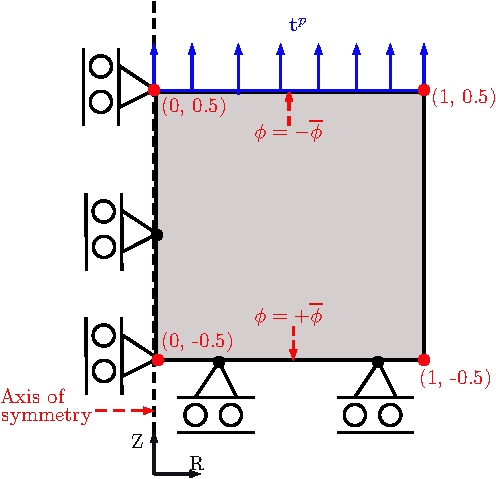
\includegraphics[width=0.78\textwidth]{coupled_unit_test_geom.pdf}
\caption{Representative geometry}
\label{fig:3.8.1}
\end{subfigure}
\begin{subfigure}{0.28\textwidth}
\centering
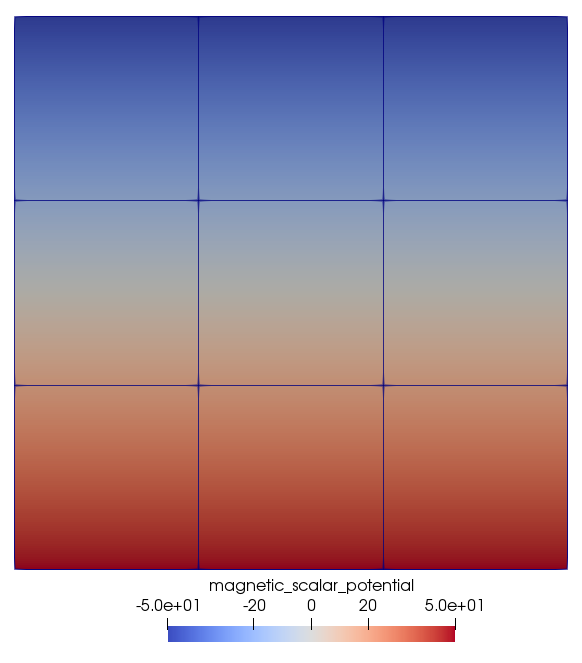
\includegraphics[width=0.95\textwidth]{coup_unit_test_mag_pot.png}
\caption{Prescribed potential $\phi$}
\label{fig:3.8.2}
\end{subfigure}
\begin{subfigure}{0.28\textwidth}
\centering
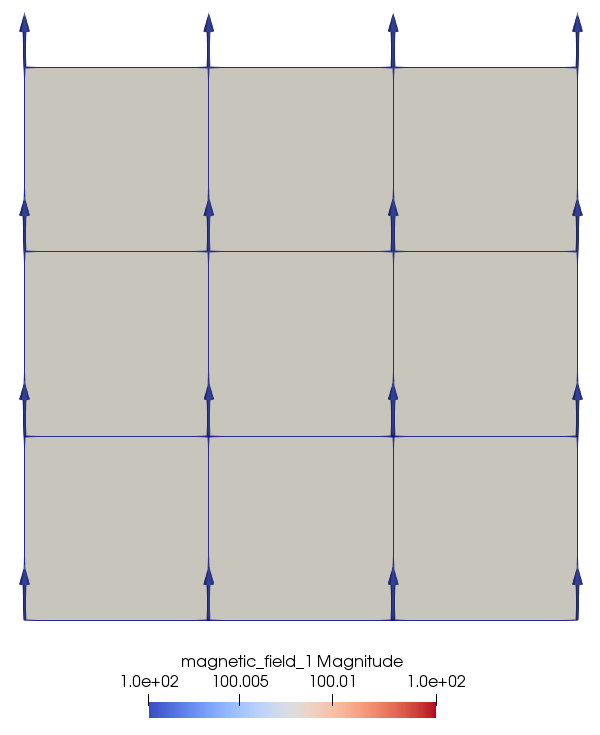
\includegraphics[width=0.9\textwidth]{coup_unit_test_mag_field.png}
\caption{Resulting $\mathbb{H}$ orientation}
\label{fig:3.8.3}
\end{subfigure}
\caption{Unit test for coupled problem}
\label{fig:3.8}
\end{figure}

\begin{table}[ht]
\centering
\begin{tabular}[c]{|C{2cm}|C{5cm}|C{5cm}|}
\hline
\textbf{{Load step}} & \textbf{{Applied magnetic potential difference}} & \textbf{{Applied mechanical traction $p_0$}} \\
\hline
25\% & 500 & 0 \\
\hline
50\% & 1000 & 0 \\
\hline
75\% & 1000 & 5e-3 \\
\hline
100\% & 1000 & 1e-2 \\
\hline 
\end{tabular} 
\caption{Load values at different load steps for coupled unit test problem}
\label{tab:3.1}
\end{table}

The constitutive law stated in \Cref{eq:3.5} was employed to describe the material response for the coupled unit test problem and the chosen values for the material parameters are $\mu = 3e^{-2}$ Pa, $\nu = 0.4$ and relative permeability $\mu_r = 6.0$. A magnetic potential difference of 1000 per unit length was applied in first half of total load cycle and a prescribed traction load $\mathbf{t}^p = 1e^{-2} \frac{\text{N}}{\text{m}}$ was applied in the second half of total load application cycle. The corresponding loads at different load steps is mentioned in \Cref{tab:3.1}. \par 

\begin{figure}[h]
\centering
\begin{subfigure}{0.23\textwidth}
\centering
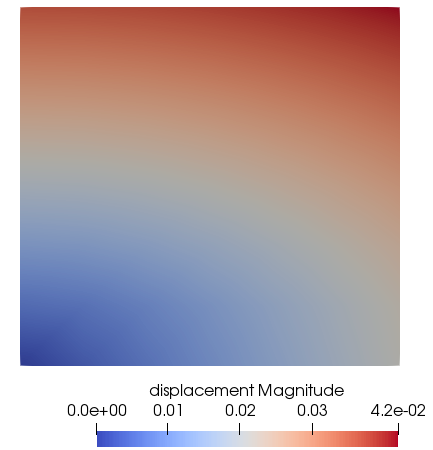
\includegraphics[width=0.85\textwidth]{unit_test_half_mag_load_disp.png}
\caption{25\% of total load}
\label{fig:3.9.1}
\end{subfigure}
\begin{subfigure}{0.24\textwidth}
\centering
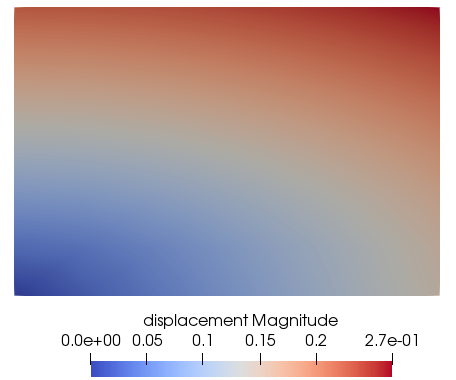
\includegraphics[width=0.8\textwidth]{unit_test_full_mag_load_disp.png}
\caption{50\% of total load}
\label{fig:3.9.2}
\end{subfigure}
\begin{subfigure}{0.24\textwidth}
\centering
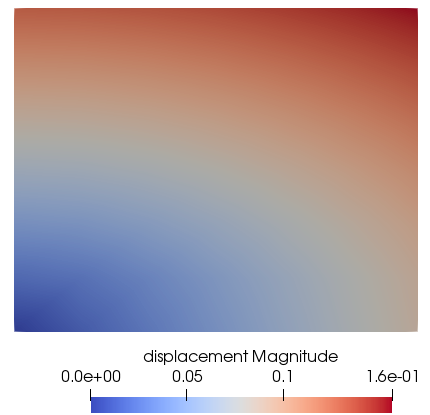
\includegraphics[width=0.8\textwidth]{unit_test_ls_15_disp.png}
\caption{75\% of total load}
\label{fig:3.9.3}
\end{subfigure}
\begin{subfigure}{0.23\textwidth}
\centering
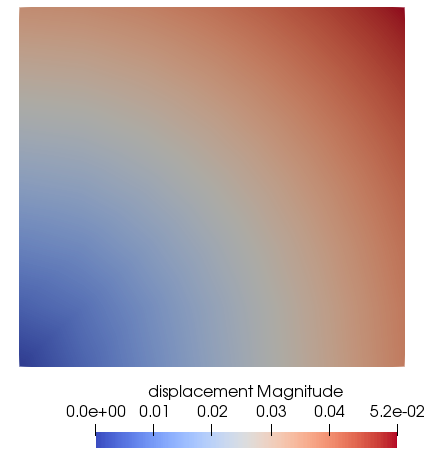
\includegraphics[width=0.85\textwidth]{unit_test_full_total_load_disp.png}
\caption{Total load}
\label{fig:3.9.4}
\end{subfigure}
\caption{Deformations of the unit cube under coupled magnetic and mechanical load (Scale of each result is to be noted)}
\label{fig:3.9}
\end{figure}

In reference to the resulting deformations at different load steps in \Cref{fig:3.9.1,fig:3.9.2}, in the first half cycle with the magnetic load application we observe the geometry undergoes compression. Due to the prescribed magnetic potentials at the top and bottom boundaries a vertically aligned magnetic field is generated as observed in \Cref{fig:3.8.3}. With no deformations in the initial reference configuration ($\mathbf{F} = \mathbf{C} = \mathbf{I}$ and $J = 1 \implies \Psi_0^{\text{elas}} = 0$) following \Cref{eq:3.5}, the S.E.F. ($M_0$) for high magnetic field $\mathbb{H}$ leads to a high negative S.E.F. Due to this effect the material softens and becomes less stiff at high magnetic loads. The material experiences a compressive load on the boundaries prescribed with the magnetic potential and this leads to a compression of the material. After the full magnetic load is applied, the material then experiences a tensile load due to the mechanical traction load applied on the top surface in the second half load cycle. For the considered material stiffness parameters, a small traction load is required to overcome the compression developed by the high magnetic load. Thus, the material extends back to its original form as observed in \Cref{fig:3.9.4}. \par 

\subsection{Dependence of material response on the direction of magnetic field}
To test the dependence of the field $\mathbb{H}$ direction on the material response, the prescribed magnetic potential was reversed, i.e. a positive potential $\phi = +\overline{\phi}$ on the top boundary and a negative potential $\phi = -\overline{\phi}$ on the bottom boundary was prescribed as seen in \Cref{fig:3.10.1}. The resulting magnetic field direction in \Cref{fig:3.10.2} is opposite when compared to \Cref{fig:3.8.3}. It was observed that irrespective of the magnetic field direction the resulting material response remained unchanged. For the reversed field direction the material experienced same compression and resulted in same deformed states as observed in \Cref{fig:3.9}. This helps understand that the alignment of the resulting magnetic field w.r.t. the axisymmetric geometry is of importance rather than the direction in which it points. It also points out that the magnetic field leads to a compressive response of the magneto-elastic material for high magnetic loads. \par 

\begin{figure}[h]
\centering
\begin{subfigure}{0.48\textwidth}
\centering
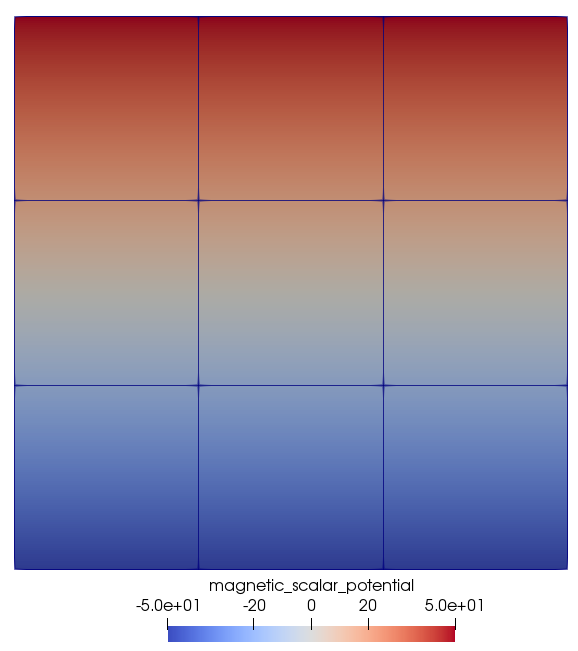
\includegraphics[width=0.6\textwidth]{coup_unit_test_mag_pot_rev.png}
\caption{Reversed potential $\phi$ prescribed}
\label{fig:3.10.1}
\end{subfigure}
\begin{subfigure}{0.48\textwidth}
\centering
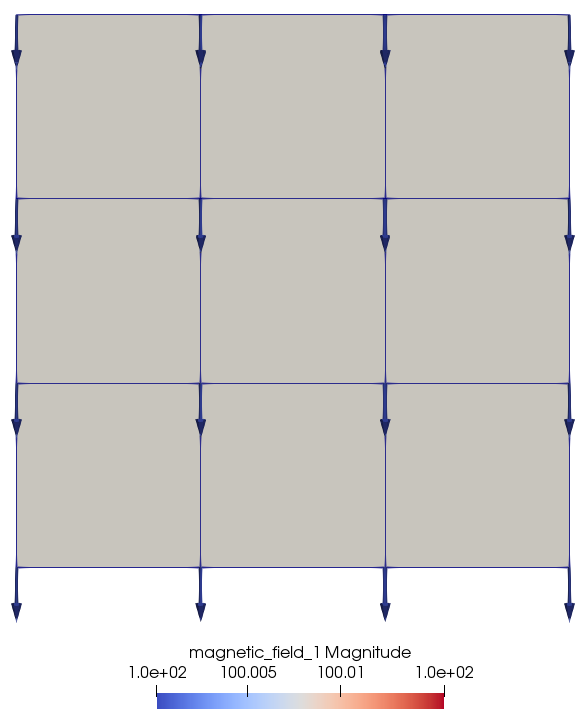
\includegraphics[width=0.6\textwidth]{coup_unit_test_mag_field_rev.png}
\caption{Resulting field $\mathbb{H}$ direction}
\label{fig:3.10.2}
\end{subfigure}
\caption{Test for reversed magnetic field direction}
\label{fig:3.10}
\end{figure}

\section{Magneto-elastic torus membrane with free space}
\label{sec:torus_problem}

We now examine the coupled problem of the torus magneto-elastic membrane with the surrounding free space as mentioned in \Cref{sec:problem_setup}. The load application explained in \Cref{sec:load_setup} is to be considered unless another load application set up is mentioned. The membrane is modelled as a non-linear hyperelastic material employing the constitutive material model \Cref{eq:3.5} with coupling between the magnetic and the elastic quantities. We consider the neighbouring free space as a complaint elastic modelled with the same material model but with relatively low elastic stiffness. The material parameters considered for the membrane are $\mu = 3e^{4}$ Pa and $\nu = 0.4$, whereas the free space material parameters considered are $\mu = 3e^1$ Pa and $\nu = 0.3$. The quasi-static inflating traction load applied was $p_0 = 1500$ Pa. A high magnetic potential difference of $3.5e^5$ per unit length was prescribed in the first half of total load cycle. The load values at different load steps are mentioned in \Cref{tab:3.2}. \par     

\begin{table}[ht]
\centering
\begin{tabular}[c]{|C{2cm}|C{5cm}|C{5cm}|}
\hline
\textbf{{Load step}} & \textbf{{Applied magnetic potential difference}} & \textbf{{Applied mechanical traction $p_0$}} \\
\hline
25\% & $1.75e^5$ & 0 \\
\hline
50\% & $3.5e^5$ & 0 \\
\hline
75\% & $3.5e^5$ & 750 \\
\hline
100\% & $3.5e^5$ & 1500 \\
\hline 
\end{tabular} 
\caption{Load values at different load steps for torus magneto-elastic membrane with free space problem}
\label{tab:3.2}
\end{table} 

\subsection{Deformations of the membrane under combined loads}

\begin{figure}[h]
\centering
\begin{subfigure}{0.48\textwidth}
\centering
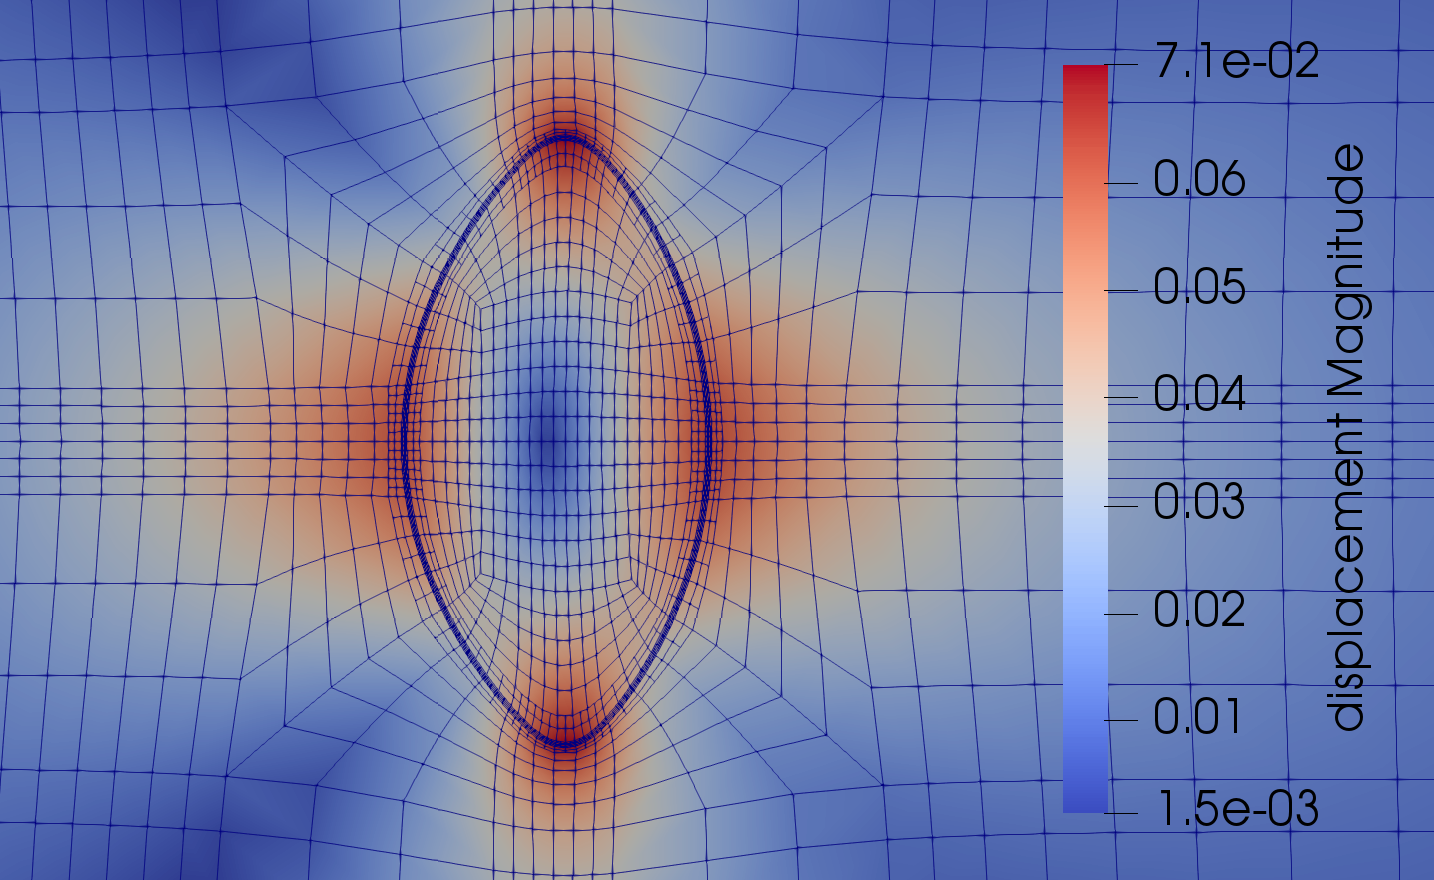
\includegraphics[width=0.85\textwidth]{coup_membrane_ls_50_disp.png}
\caption{Half load (total magnetic load applied)}
\label{fig:3.11.1}
\end{subfigure}
\begin{subfigure}{0.48\textwidth}
\centering
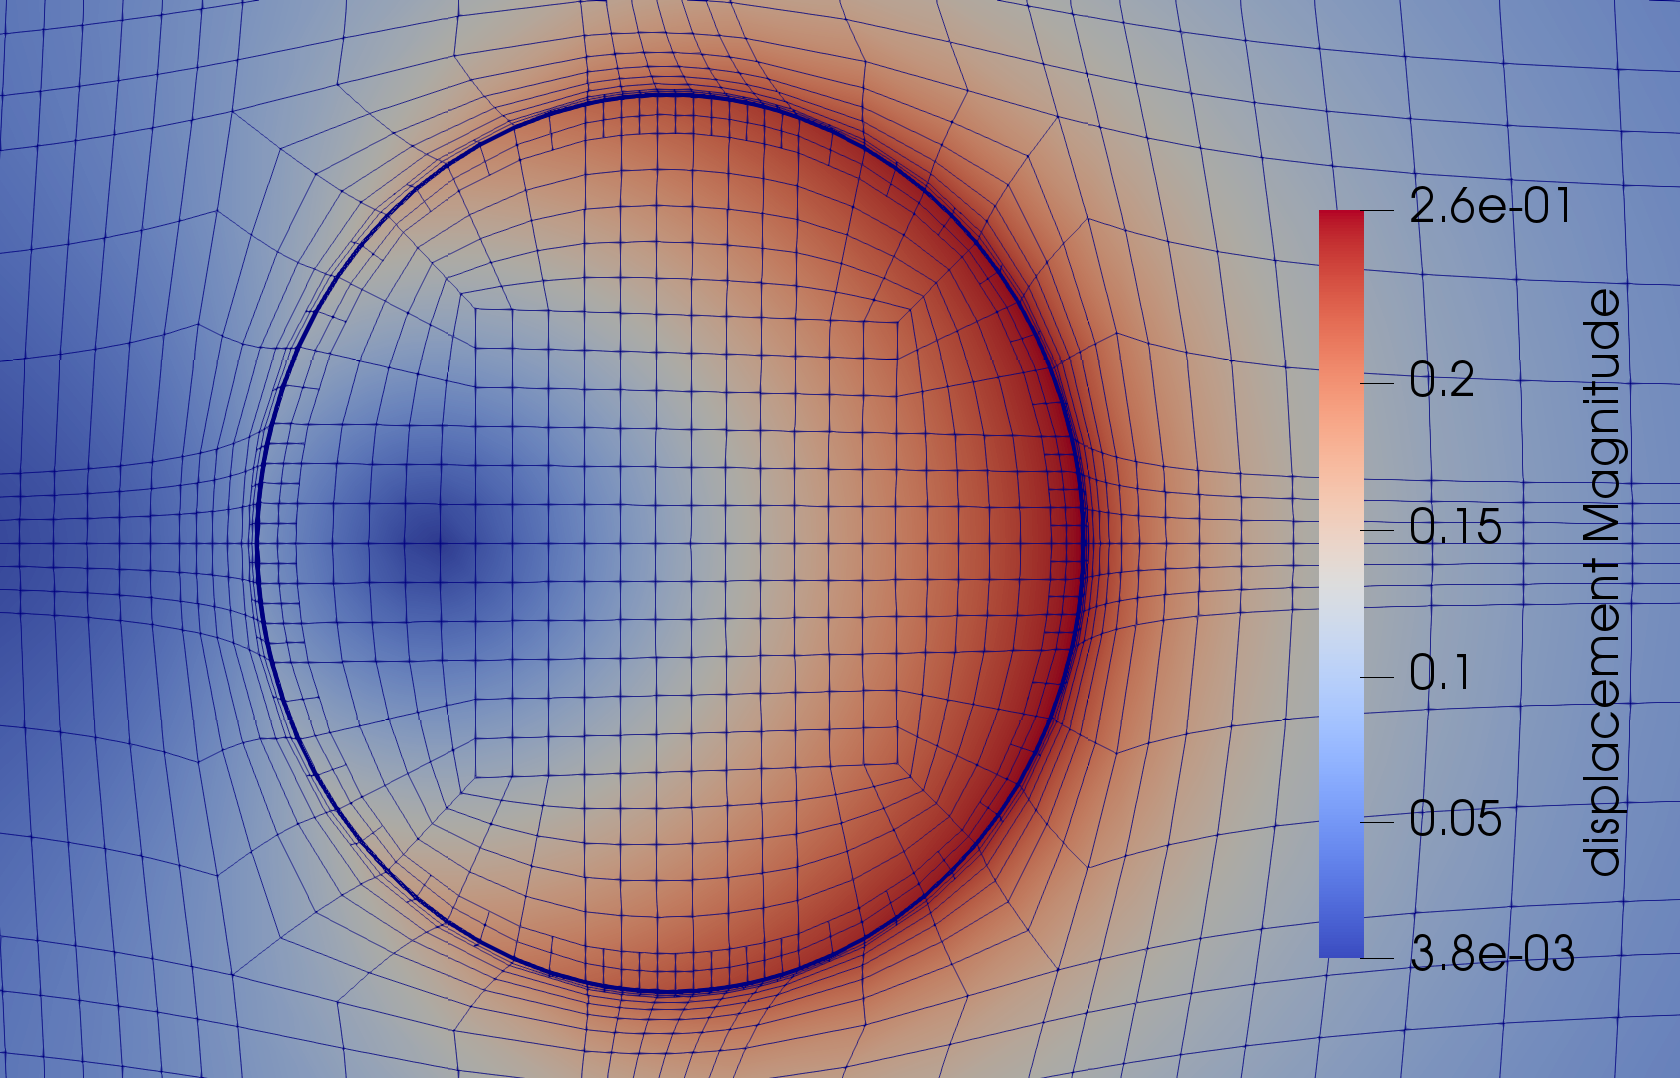
\includegraphics[width=0.8\textwidth]{coup_membrane_ls_100_disp.png}
\caption{Full load (total magnetic and mechanical load)}
\label{fig:3.11.2}
\end{subfigure}
\caption{Deformations of the membrane and neighbouring free space for coupled problem}
\label{fig:3.11}
\end{figure}

We observe the deformed states of the domain at the end of the magnetic load application  in \Cref{fig:3.11.1} and at the end of the total magnetic and mechanical load application in \Cref{fig:3.11.2}, respectively. As found out from the unit test result in \Cref{sec:unit_test_coup}, on the application of high magnetic loads the material undergoes compression for the vertically aligned magnetic field. We observe a similar effect on the magneto-elastic membrane in the first half of total load cycle (linearly increasing magnetic load and zero mechanical load). The membrane undergoes finite deformations in the lateral and longitudinal directions. The centre of the membrane shifts by negligible magnitude along the radial direction. The membrane thickness also has negligible change at this state. The displacements in the membrane sections along the cylindrical co-ordinate axes direction are significantly high compared to the other sections. \par 
In the second phase of loading, the membrane starts to inflate on the application of high inflating pressure load, c.f. \Cref{fig:3.11.2}. The applied high traction load overcomes the effect of the compressive forces developed by the magnetic load. The membrane expands back to a circular topology within first few traction application load steps. On further load application, the membrane then inflates to a larger radius. The torus minor radius at the end of total load application has increased from 0.195 m to $\approx$ 0.38 m. The centre of the torus has also shifted by a significant distance of 0.1 m to the right. The membrane thickness due to the large stretch has reduced from $5e^{-3}$ m to $\approx 2.8e^{-3}$ m. As was explained in the quasi-static finite strain elasticity results in Task 2.1, the deformations on the right half of the circular cross-section are relatively large compared to the left half. This is due to the dependence of $\mathbf{F}$ (component $F_{33}$) on the radial distance of the respective point from the axis of symmetry. \par 

It is important to note that the current load values were chosen to demonstrate the finite deformations the membrane can undergo before the onset of any mechanical instability in the membrane (or the complaint free space). On further increasing the magnetic and mechanical pressure load, it was observed that either the Newton solver would not converge or we would observe material instability in the free space elements in close vicinity to the deforming membrane. \par 

\subsection{Developed magnetic field inside the membrane}

\begin{figure}[h]
\centering
\begin{subfigure}{0.32\textwidth}
\centering
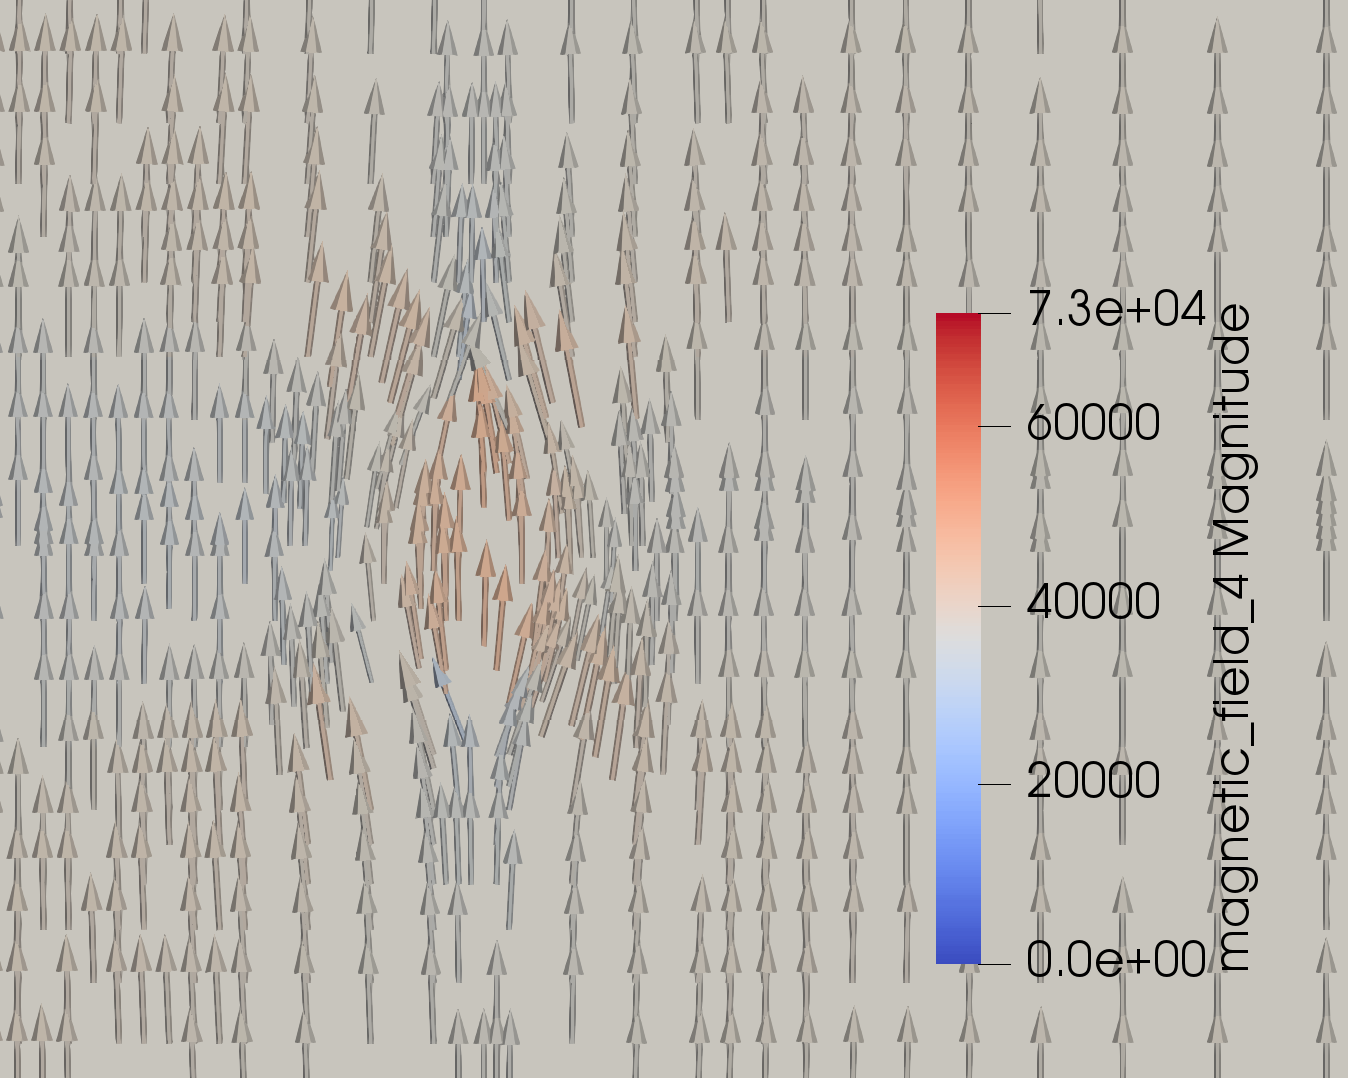
\includegraphics[width=0.9\textwidth]{coup_membrane_field_ls_50.png}
\caption{50\% of total load}
\label{fig:3.12.1}
\end{subfigure}
\begin{subfigure}{0.32\textwidth}
\centering
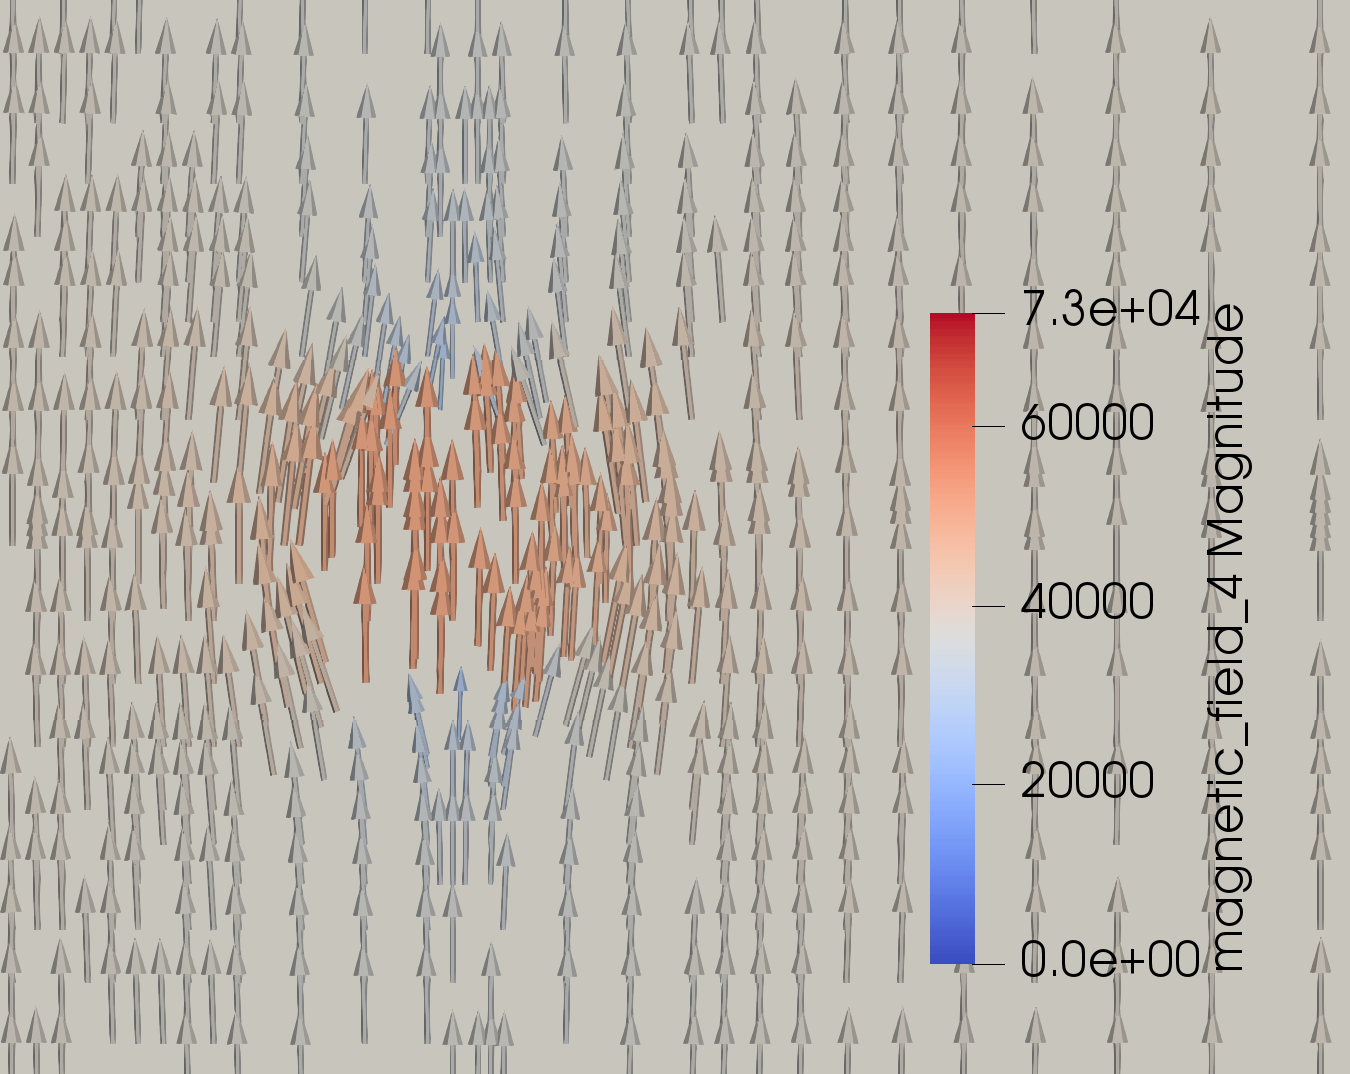
\includegraphics[width=0.9\textwidth]{coup_membrane_field_ls_75.png}
\caption{75\% of total load}
\label{fig:3.12.2}
\end{subfigure}
\begin{subfigure}{0.32\textwidth}
\centering
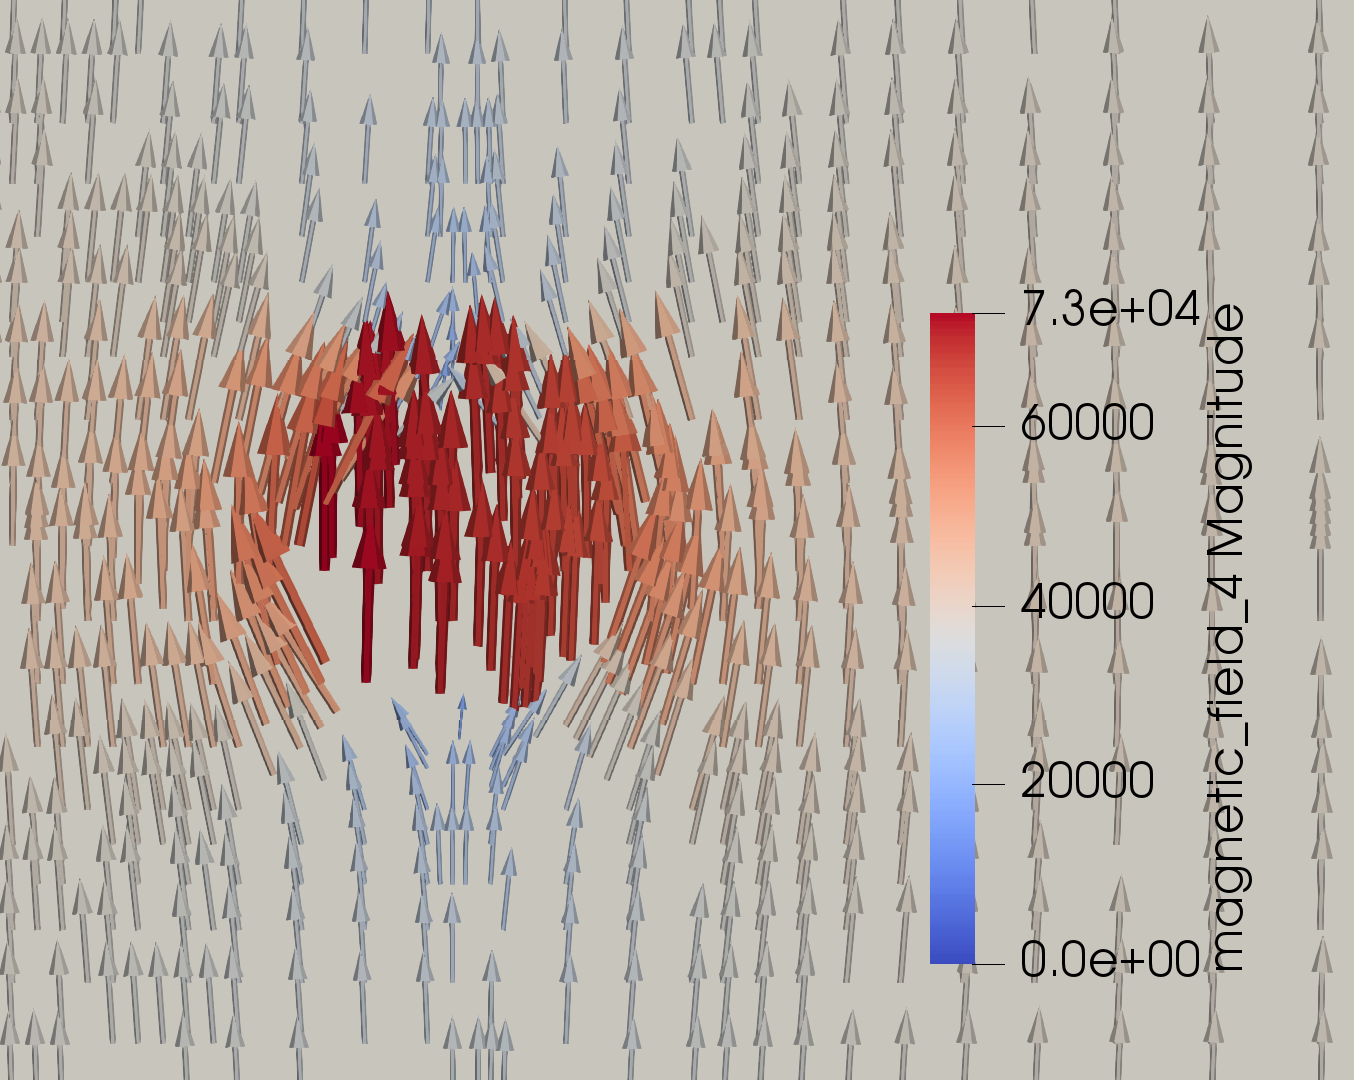
\includegraphics[width=0.9\textwidth]{coup_membrane_field_ls_100.png}
\caption{Total load}
\label{fig:3.12.3}
\end{subfigure}
\caption{Resulting magnetic field $\mathbb{H}$ in \textbf{free space around magneto-elastic membrane} in second half of load cycle (constant (full) magnetic load and linearly increasing mechanical traction load)}
\label{fig:3.12}
\end{figure}

\begin{figure}[h]
\centering
\begin{subfigure}{0.32\textwidth}
\centering
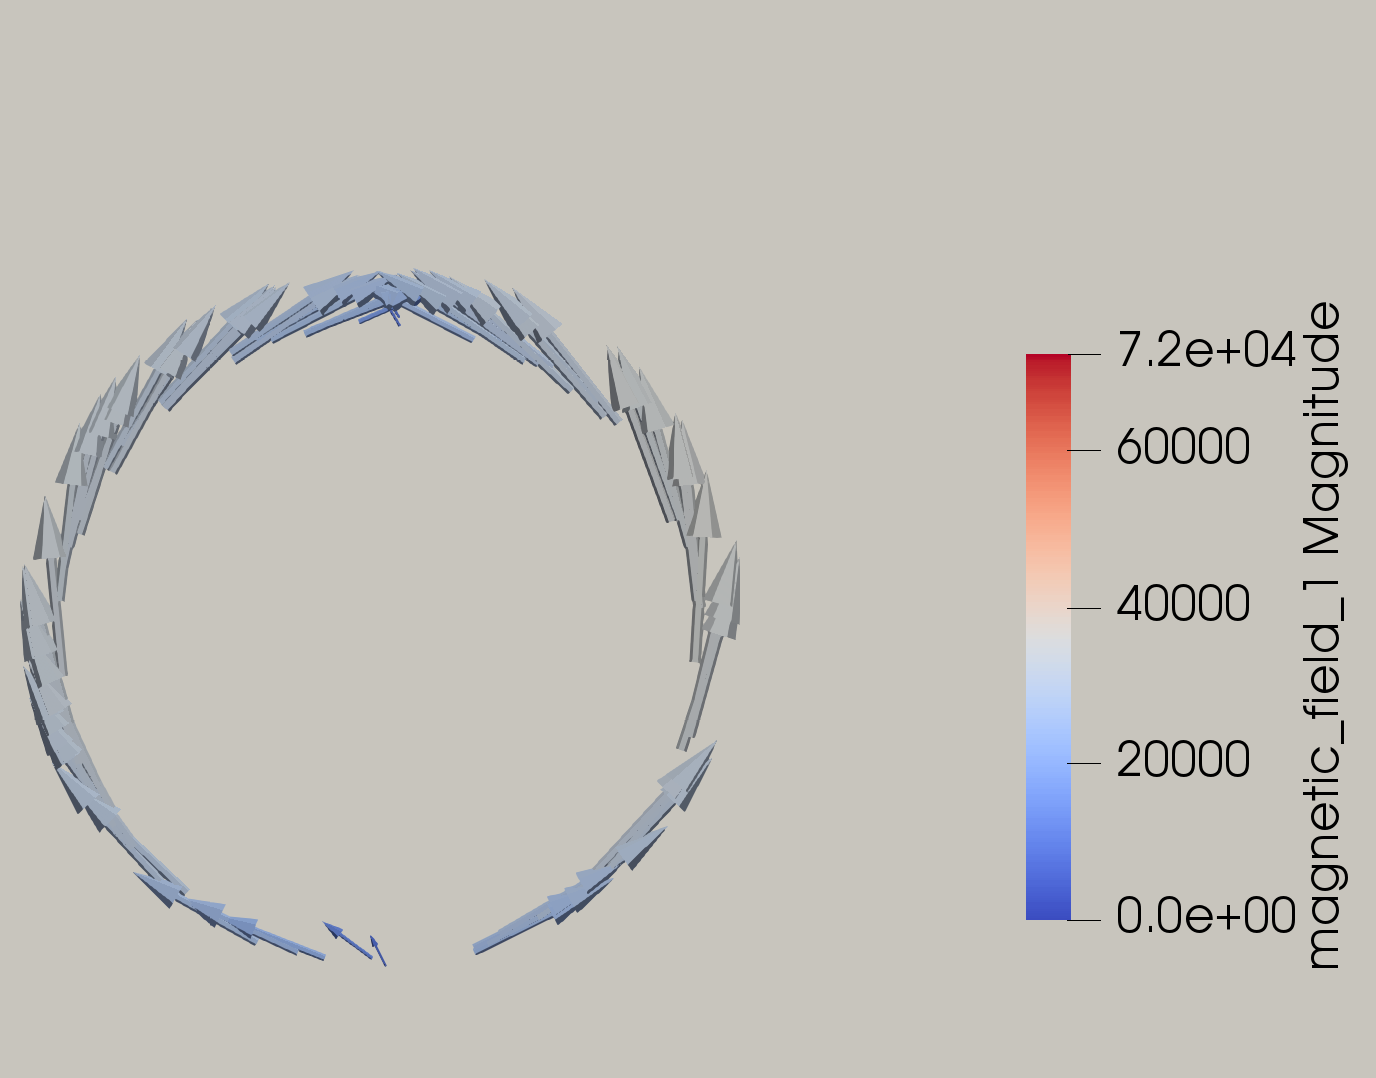
\includegraphics[width=0.9\textwidth]{coup_mag_field_membrane_ls_50.png}
\caption{50\% of total load}
\label{fig:3.14.1}
\end{subfigure}
\begin{subfigure}{0.32\textwidth}
\centering
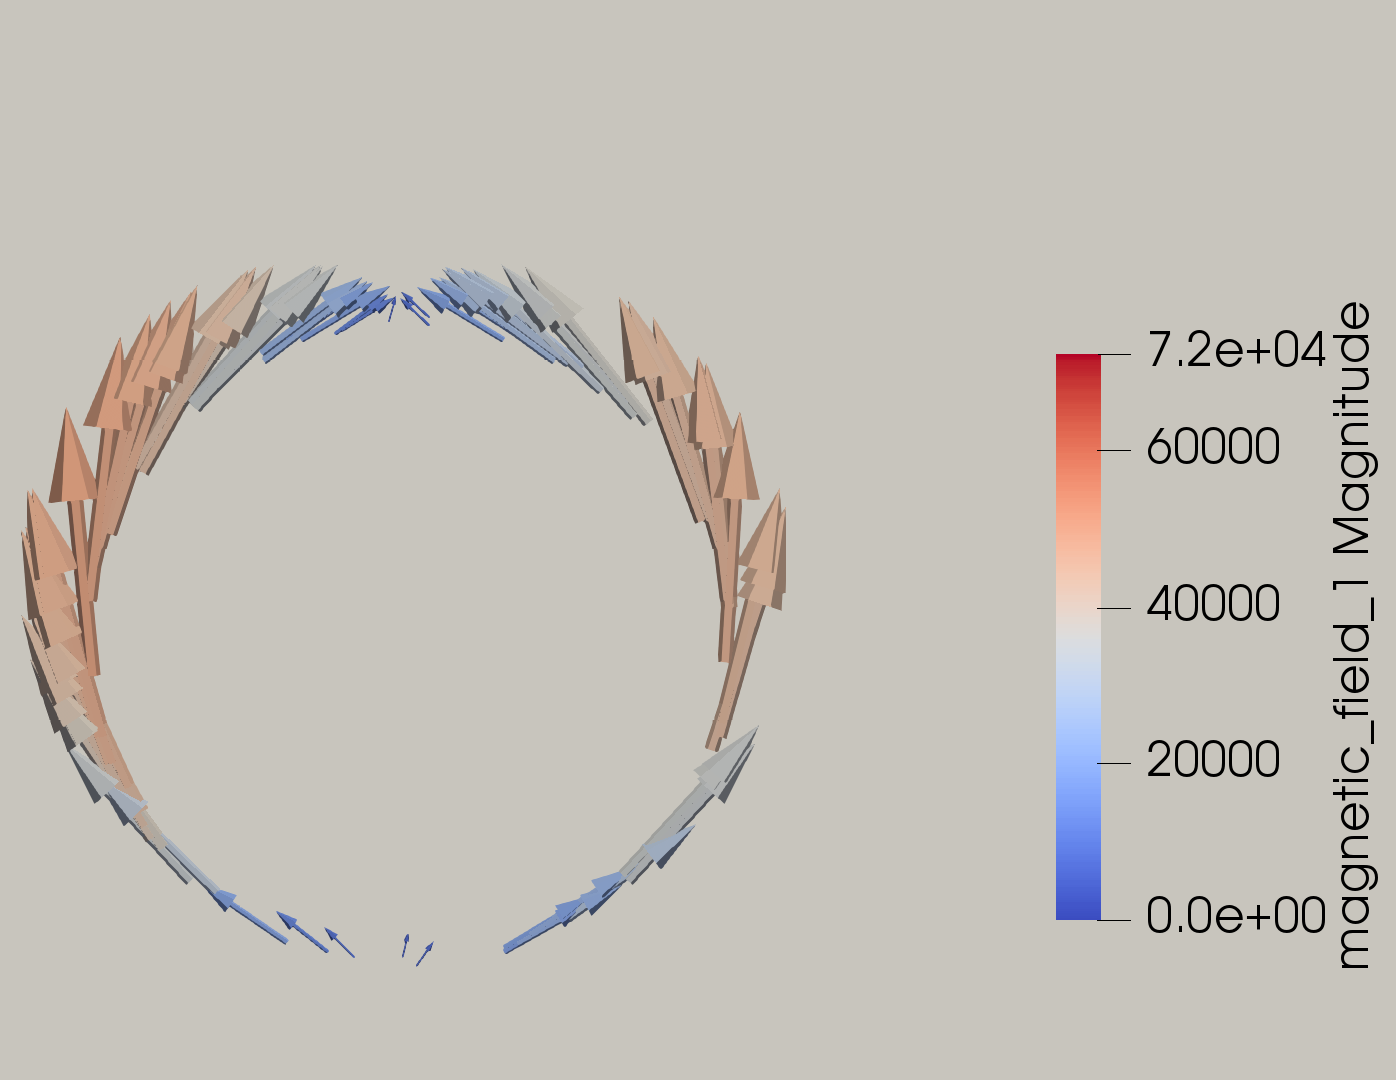
\includegraphics[width=0.9\textwidth]{coup_mag_field_membrane_ls_75.png}
\caption{75\% of total load}
\label{fig:3.14.2}
\end{subfigure}
\begin{subfigure}{0.32\textwidth}
\centering
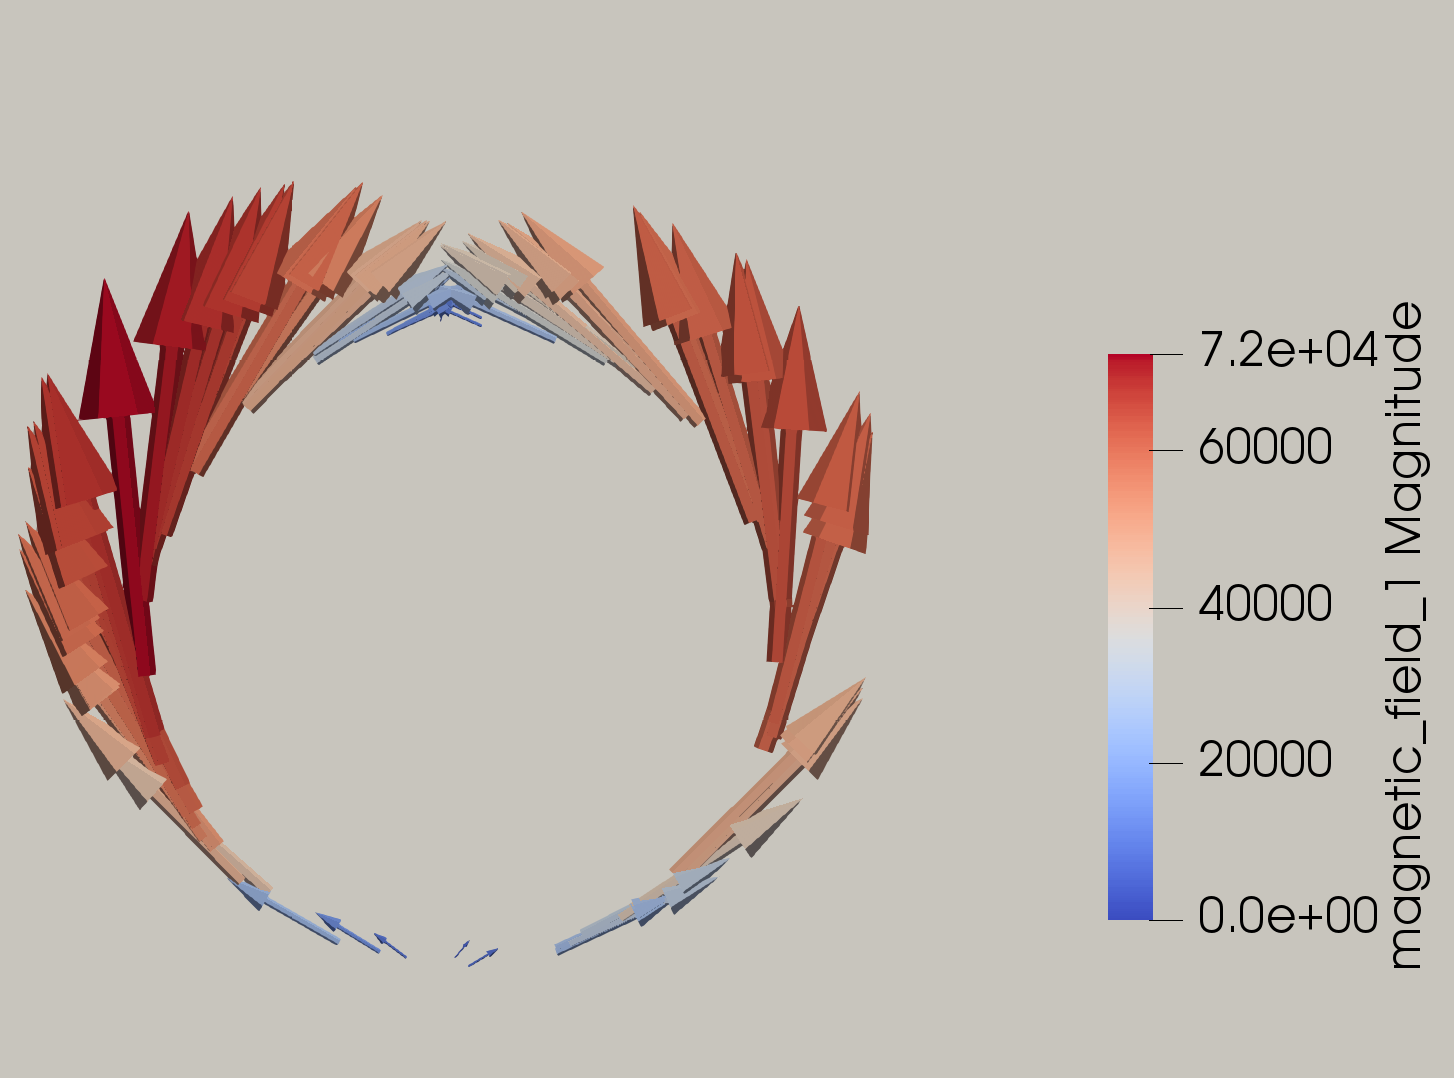
\includegraphics[width=0.9\textwidth]{coup_mag_field_membrane_ls_100.png}
\caption{Total load}
\label{fig:3.14.3}
\end{subfigure}
\caption{Resulting magnetic field $\mathbb{H}$ in \textbf{magneto-elastic membrane} in second half of load cycle (constant (full) magnetic load and linearly increasing mechanical traction load)}
\label{fig:3.14}
\end{figure}

We now examine the developed magnetic field in the region close to the membrane in \Cref{fig:3.12} and within the membrane in \Cref{fig:3.14}. The magnetic field generated in the first half cycle after total magnetic potential is prescribed can be observed in \Cref{fig:3.12.1}. As seen in the representative load application cycle \Cref{tab:3.2}, in the second half cycle we do not further increase the applied magnetic load. Rather, the mechanical load application begins in the second phase of loading. From the results shown in \Cref{fig:3.12.2,fig:3.12.3} it is evident that the magnetic field inside the membrane, region enclosed within the membrane and surrounding the membrane increases. The increase in the magnetic field can be attributed to the self-magnetization of the magneto-elastic membrane as observed in \Cref{fig:3.14.2,fig:3.14.3}. The resulting magnetic field due to the self-magnetization of the membrane is aligned with the field generated by the application of potential $\phi$. This causes the effective field to increase and thus we observe an increased magnitude of the total magnetic field with no increase in external magnetic load. The magnetic field increase in magnitude after total magnetic and mechanical load application (100\% load) is two-folds compared to the field after the application of total magnetic load only (50\% load). \par 

\subsection{Comparative study of deformations under two different load set ups}

To demonstrate the finite deformations of the membrane for the considered loads of chosen values, we now study the deformations under a reversed load application cycle. Until now we have employed the method mentioned in \Cref{sec:load_setup} in \Cref{fig:3.6.2}. We shall refer to this as `Load set up 1'. We now consider another load application cycle with the mechanical load applied in initial phase followed by the magnetic load; here referred to as `Load set up 2'. We examine the deformed states of the magneto-elastic membrane under the two different load set ups. It is important to note that the magnitude of magnetic and the mechanical loads are kept same (as mentioned in \Cref{sec:torus_problem}) but the order of application of the respective loads is changed. The load values for `Load set up 2' are mentioned in \Cref{tab:3.3}. \par 

\begin{table}[ht]
\centering
\begin{tabular}[c]{|C{2cm}|C{5cm}|C{5cm}|}
\hline
\textbf{{Load step}} & \textbf{{Applied magnetic potential difference}} & \textbf{{Applied mechanical traction $p_0$}} \\
\hline
25\% & 0 & 750 \\
\hline
50\% & 0 & 1500 \\
\hline
75\% & $1.75e^5$ & 1500 \\
\hline
100\% & $3.5e^5$ & 1500 \\
\hline 
\end{tabular} 
\caption{Load values for reversed load cycle in the torus magneto-elastic membrane with free space problem}
\label{tab:3.3}
\end{table} 

\begin{figure}[h]
\centering
\begin{subfigure}{0.24\textwidth}
\centering
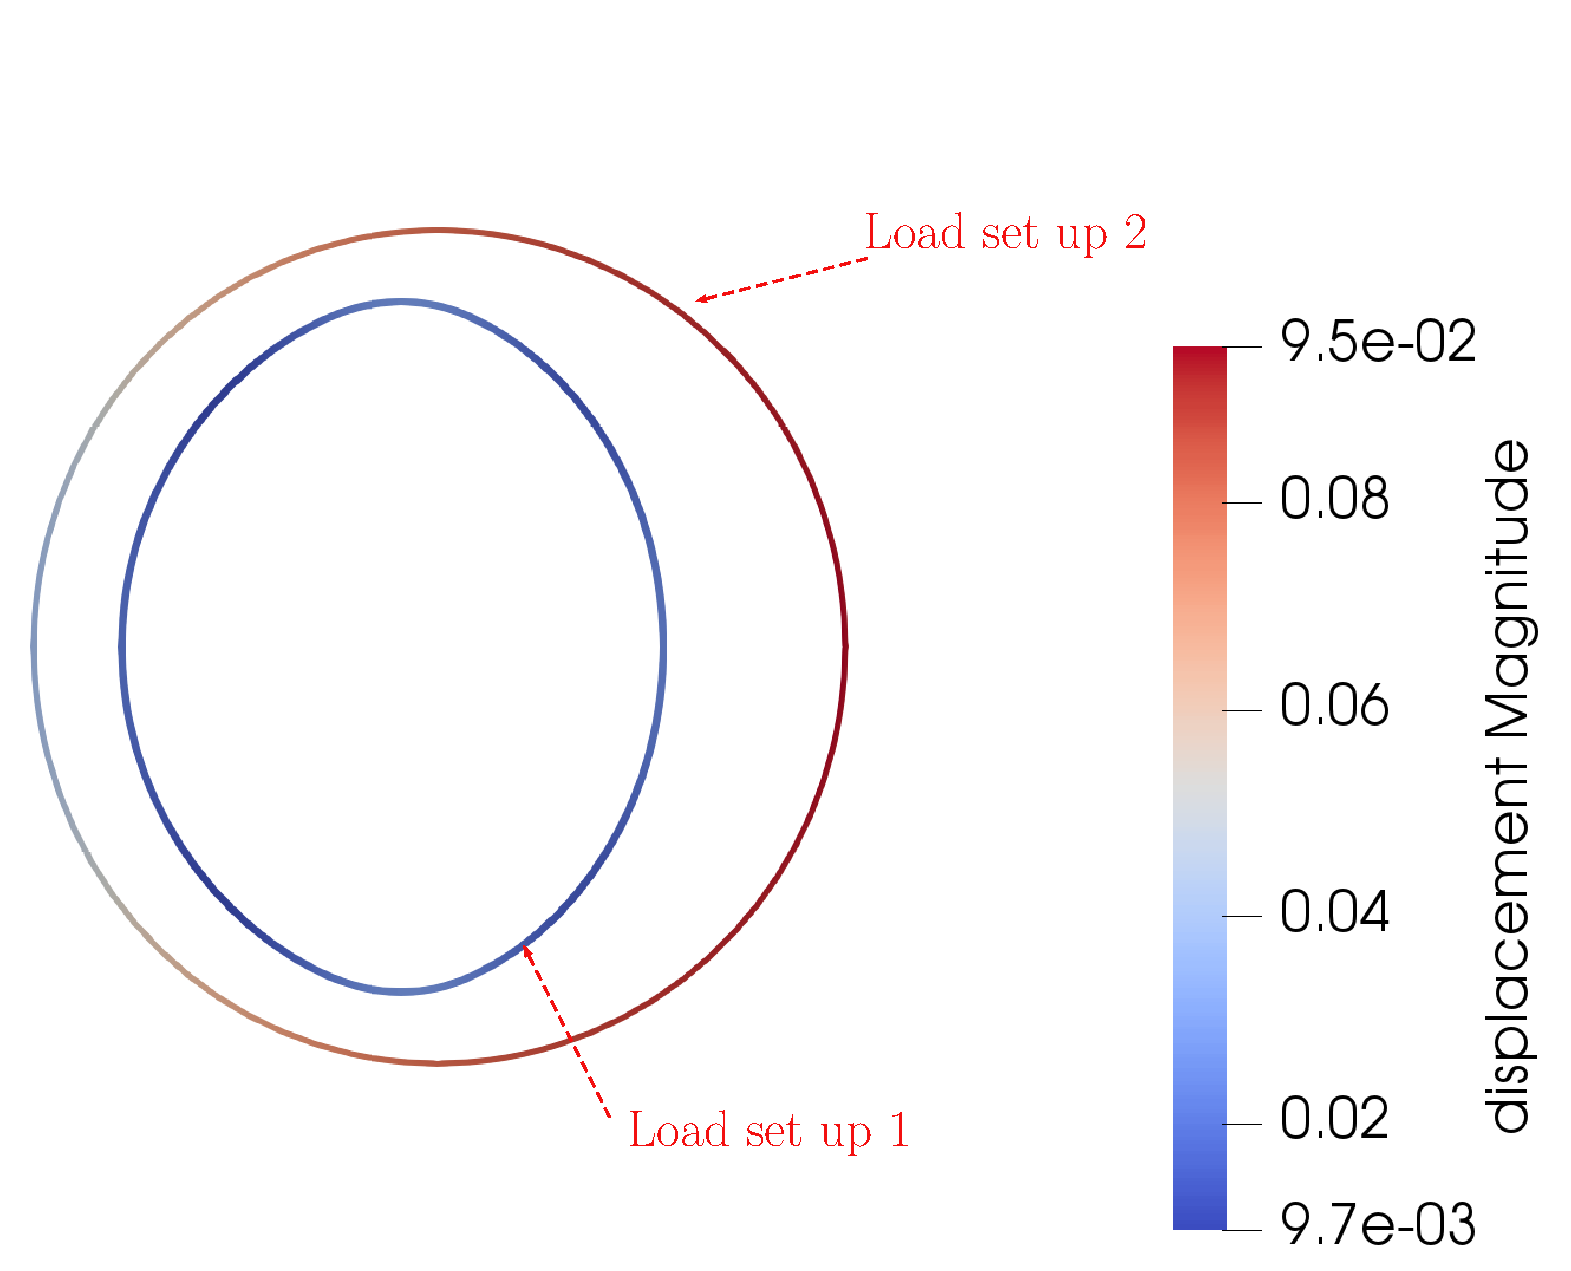
\includegraphics[width=0.9\textwidth]{torus_ls_25_mech_mag.pdf}
\caption{25\% of total load}
\label{fig:3.13.1}
\end{subfigure}
\begin{subfigure}{0.24\textwidth}
\centering
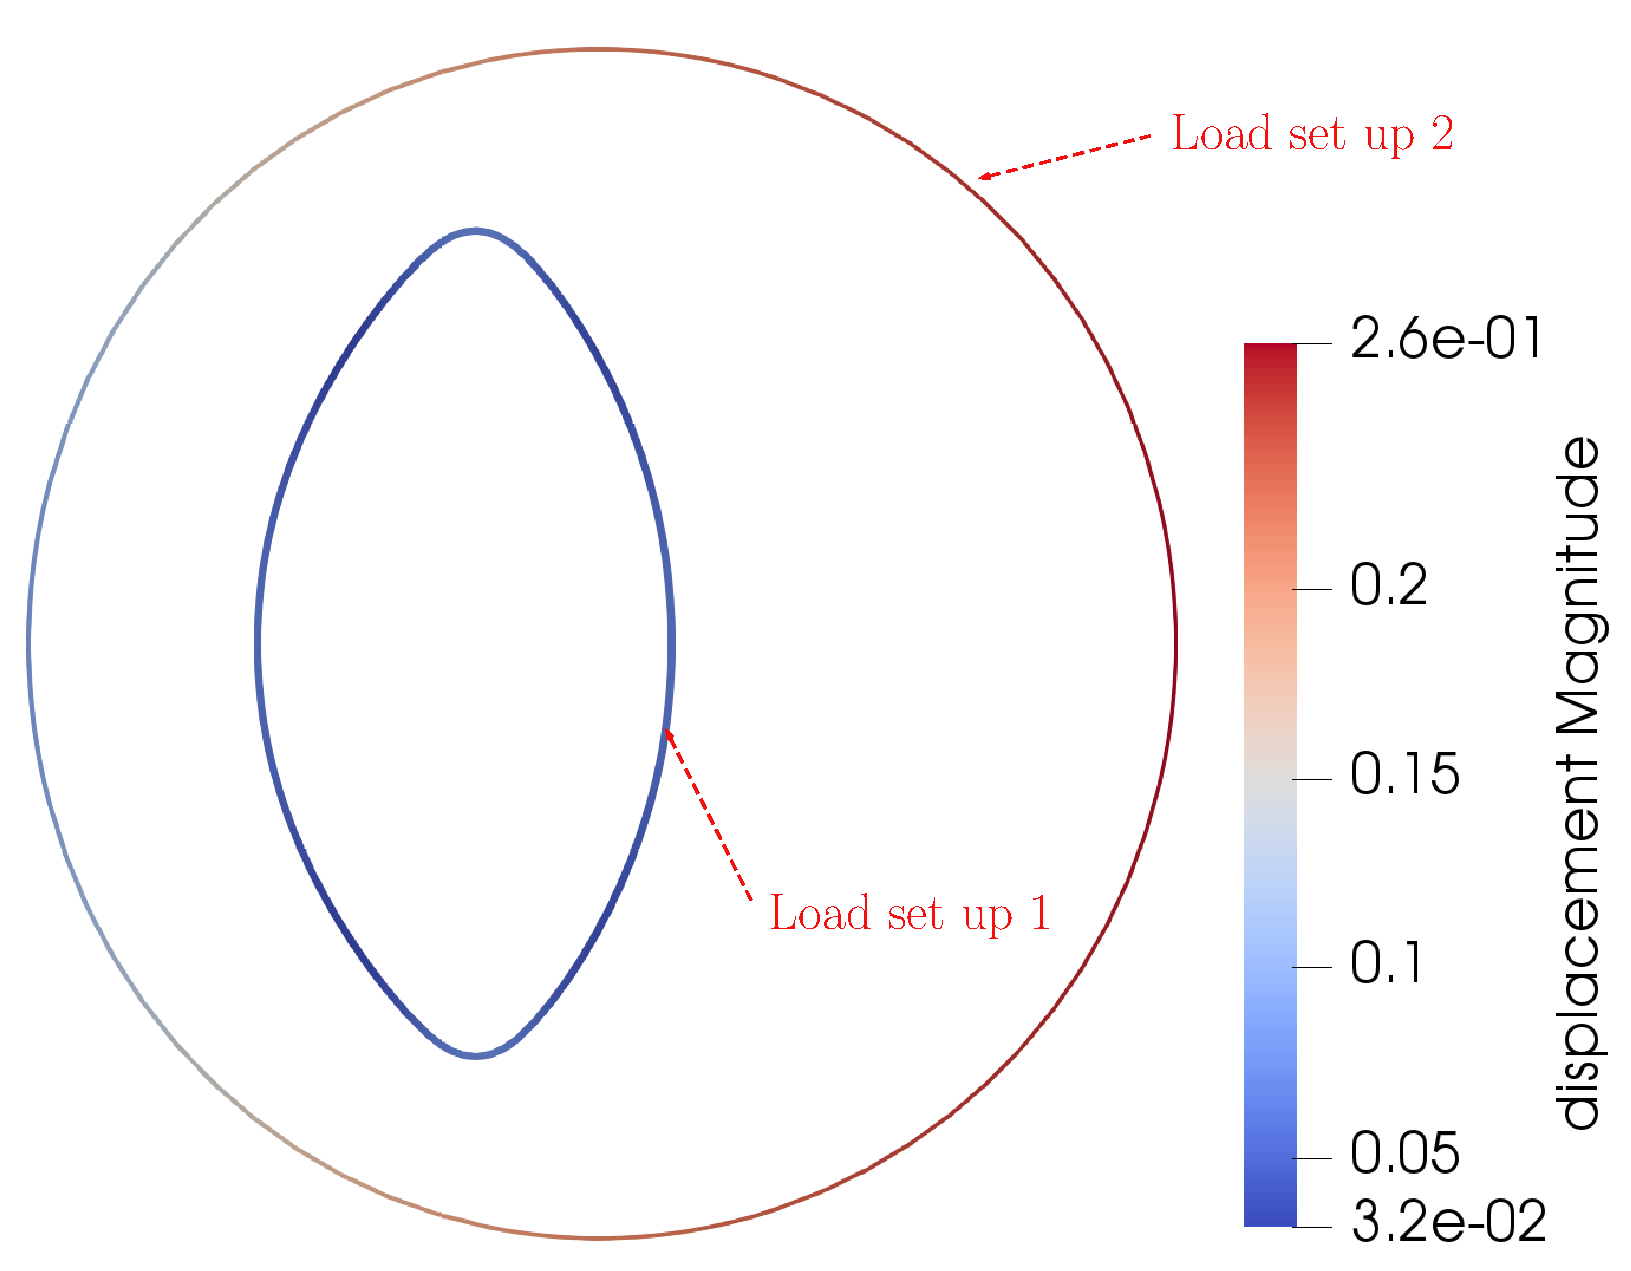
\includegraphics[width=0.9\textwidth]{torus_ls_50_mech_mag.pdf}
\caption{50\% of total load}
\label{fig:3.13.2}
\end{subfigure}
\begin{subfigure}{0.24\textwidth}
\centering
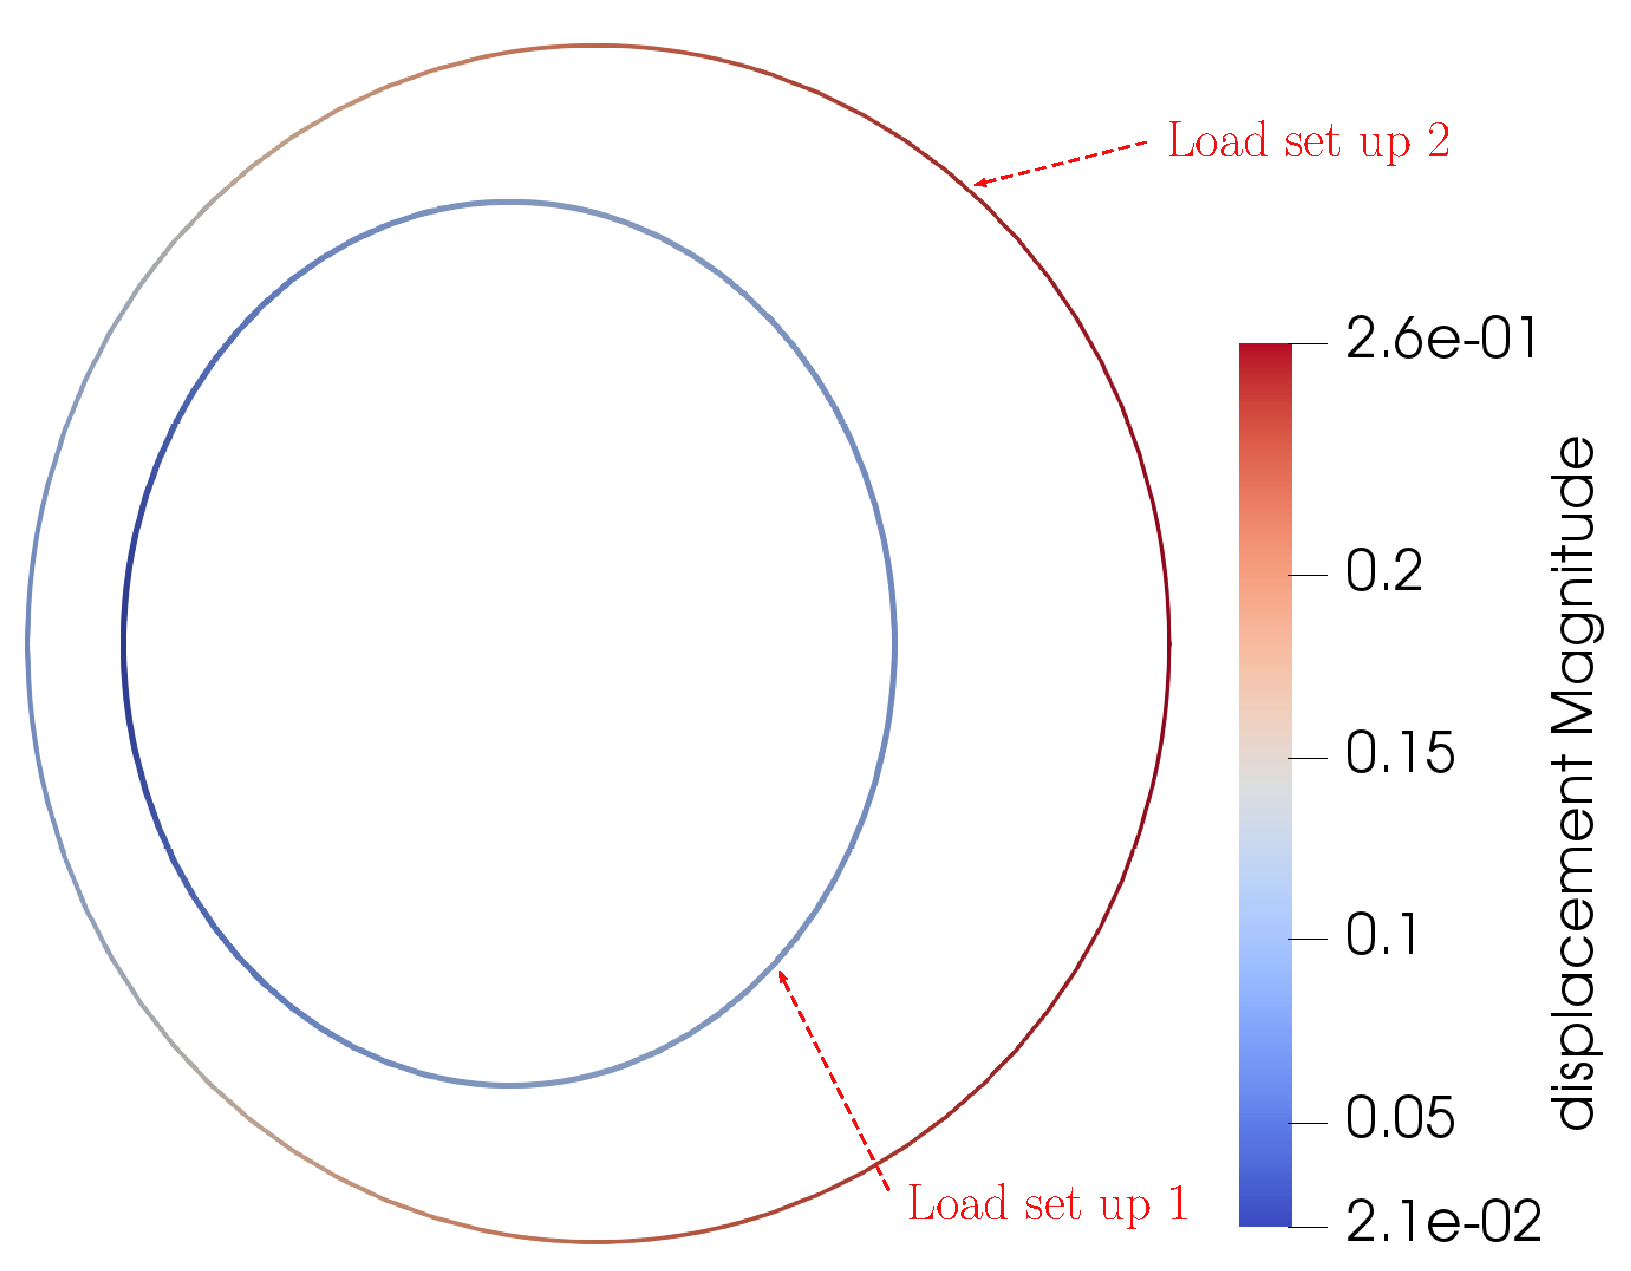
\includegraphics[width=0.9\textwidth]{torus_ls_75_mech_mag.pdf}
\caption{75\% of total load}
\label{fig:3.13.3}
\end{subfigure}
\begin{subfigure}{0.24\textwidth}
\centering
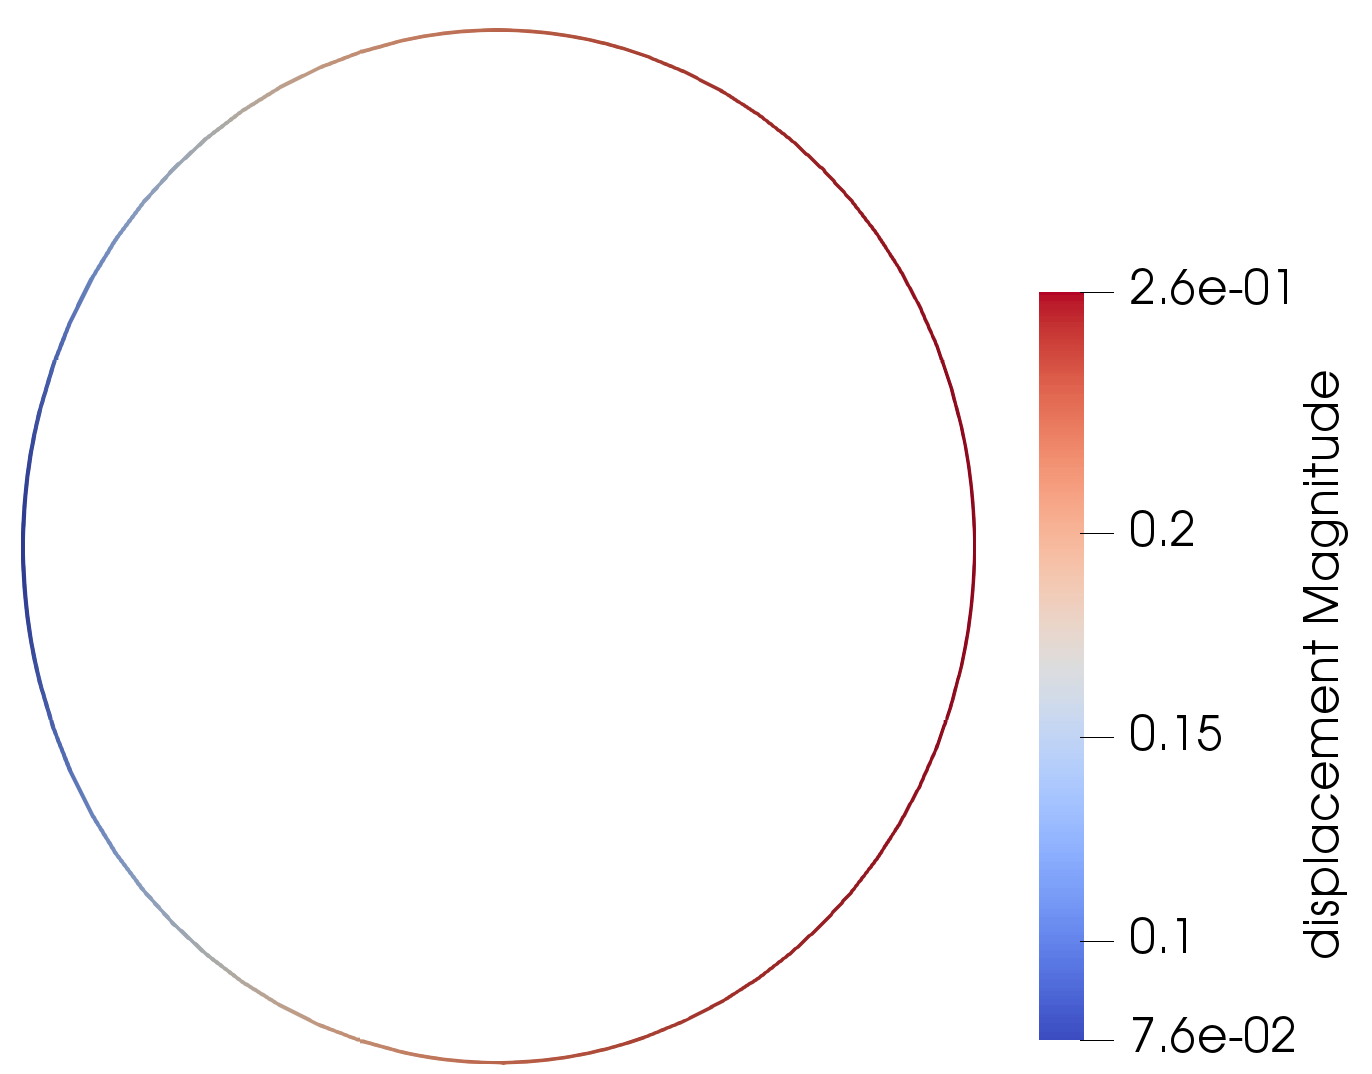
\includegraphics[width=0.9\textwidth]{torus_ls_100_mech_mag.png}
\caption{Total load}
\label{fig:3.13.4}
\end{subfigure}
\caption{Comparison between deformed states of magneto-elastic membrane for two different (equal in magnitude) load application set ups}
\label{fig:3.13}
\end{figure}

We observe the comparative results for the deformed states of the membrane at different load steps in \Cref{fig:3.13}. One can easily identify the differences in the results under different load set up from \Cref{fig:3.13.1,fig:3.13.2,fig:3.13.3}. It is interesting to point out that irrespective of the order in which one applies the loads (before any material instability is observed), the final deformed states for both the load set ups are exactly identical as observed in \Cref{fig:3.13.4}. The resulting stresses developed in the membrane under both the load set ups matched and also verified the correctness of the result observed in \Cref{fig:3.13.4}. For the `Load set up 2', it is evident that the applied magnetic load in second phase is not large enough to observe finite deformations of the new inflated membrane geometry. \par

We compare the load-displacement history for two points on the membrane inner radius in \Cref{fig:3.15}. First point is at the position (1.095, 0) located at $\Theta = \ang{0}$ (on the right section of the membrane) and the second point of interest is at position (0.9, 0.195) located at $\Theta = \ang{90}$, both measured anti-clockwise respectively. Though the equilibrium paths for both the load set ups are different, the final displacements in both the cases are same. It is important to note that the equilibrium path in the second phase of loading in `Load set up 1' is linearly increasing, thus indicating that the observed large deformations are still in stable regime and that the elastic critical limit point at which the tangent stiffness approaches to zero, hasn't arrived yet. Thus, we do not observe any buckling instability for the considered load values. For the further instability modes study, we shall continue with the `Load set up 1' where the magnetic load is applied in first phase. \par  

\begin{figure}[h]
\begin{subfigure}[t]{0.49\linewidth}
\centering
\resizebox{\linewidth}{!}{
\begin{tikzpicture}
\begin{axis}[
xlabel = $\text{Displacement (L2 norm)}$,
ylabel = $\text{Load step value}$,
%grid =both,
%grid style=dashed,
%minor grid style ={gray!30},
%major grid style ={gray!30},
%width=0.8\linewidth,
legend pos=north west,
]
\addplot[
color=red,
mark=x,
mark size=2pt,
line width=1pt,
]
table[x=Disp_norm,y=Load_value]{mag_first_point_1.dat};
\addlegendentry{Load set up 1}
\addplot[
color=blue,
mark=+,
mark size=2pt,
line width=1pt,
]
table[x=Disp_norm,y=Load_value]{mech_first_point_1.dat};
\addlegendentry{Load set up 2}
\end{axis}
\end{tikzpicture}
}
\caption{Point 1 at $\Theta = \ang{0}$}
\label{fig:3.15.1}
\end{subfigure}
\begin{subfigure}[t]{0.49\linewidth}
\centering
\resizebox{\linewidth}{!}{
\begin{tikzpicture}
\begin{axis}[
xlabel = $\text{Displacement (L2 norm)}$,
ylabel = $\text{Load step value}$,
%grid =both,
%grid style=dashed,
%minor grid style ={gray!30},
%major grid style ={gray!30},
%width=0.8\linewidth,
legend pos=north west,
]
\addplot[
color=red,
mark=x,
mark size=2pt,
line width=1pt,
]
table[x=Disp_norm,y=Load_value]{mag_first_point_2.dat};
\addlegendentry{Load set up 1}
\addplot[
color=blue,
mark=+,
mark size=2pt,
line width=1pt,
]
table[x=Disp_norm,y=Load_value]{mech_first_point_2.dat};
\addlegendentry{Load set up 2}
\end{axis}
\end{tikzpicture}
}
\caption{Point 2 at $\Theta = \ang{90}$}
\label{fig:3.15.2}
\end{subfigure}
\caption{Equilibrium paths}
\label{fig:3.15}
\end{figure}

\subsection{Study of unstable deformations of the membrane}

The thickness of a structure affects the bending stiffness of the structure. Bending stiffness is the resistance offered by the structure against any bending deformation. It is a function of the elastic modulus \textit{E} of the structure and the second moment area (also known as area moment of inertia) \textit{I} of the structure cross-section about the axis of interest. Bending stiffness in beams is also termed as \textbf{Flexural rigidity}. Since the second moment area \textit{I} depends on the cross-section dimensions of the structure, thickness of the structure thus plays a role in observing the buckling unstable deformations of our interest. Thus, to study the membrane unstable deformations leading to the buckling of the membrane we consider a membrane of reduced thickness. The magneto-elastic membrane thickness was reduced by half to 0.0025 m. The corresponding membrane minor inner and outer radii are 0.195 m and 0.1975 m, respectively. The reduced thickness of membrane was spatially discretized into four elements along the thickness to get high accuracy of the results in the membrane when observing the buckling behaviour.  \par 

The material parameters were taken as mentioned earlier in \Cref{sec:torus_problem}. For the results to be observed, an externally applied magnetic potential difference of $3e^5$ per unit length was considered and the traction load was set to $p_0 = 1500$ Pa. As mentioned earlier, the buckling deformations of our interest are observed for an established magnetic field $\mathbb{H}$ and with increasing large mechanical pressure loads \cite{reddy_toroid,Reddy2018}. Therefore we consider the load set up with the magnetic potential application in first phase. \par 


\begin{figure}[h]
\centering
\begin{subfigure}{0.3\textwidth}
\centering
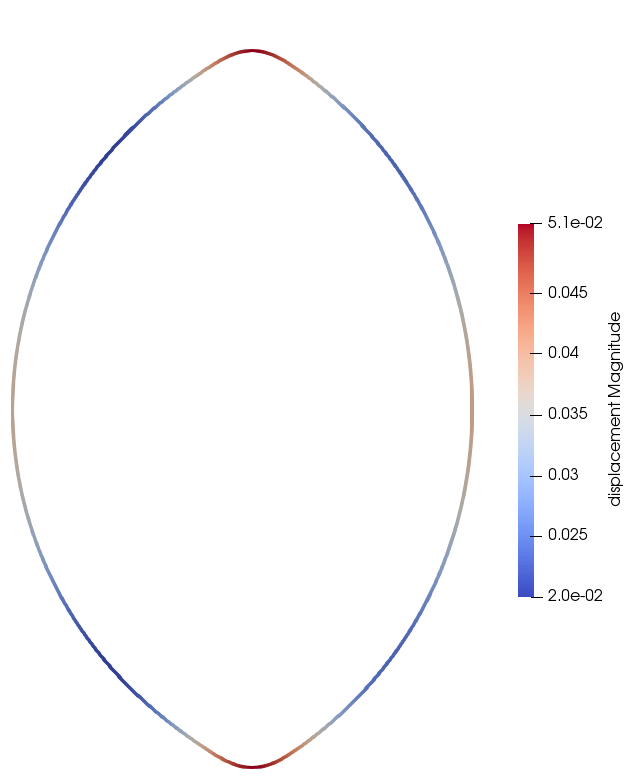
\includegraphics[width=0.85\textwidth]{instab_test_1_before_failure.png}
\caption{Before numerical failure}
\label{fig:3.16.1}
\end{subfigure}
\begin{subfigure}{0.3\textwidth}
\centering
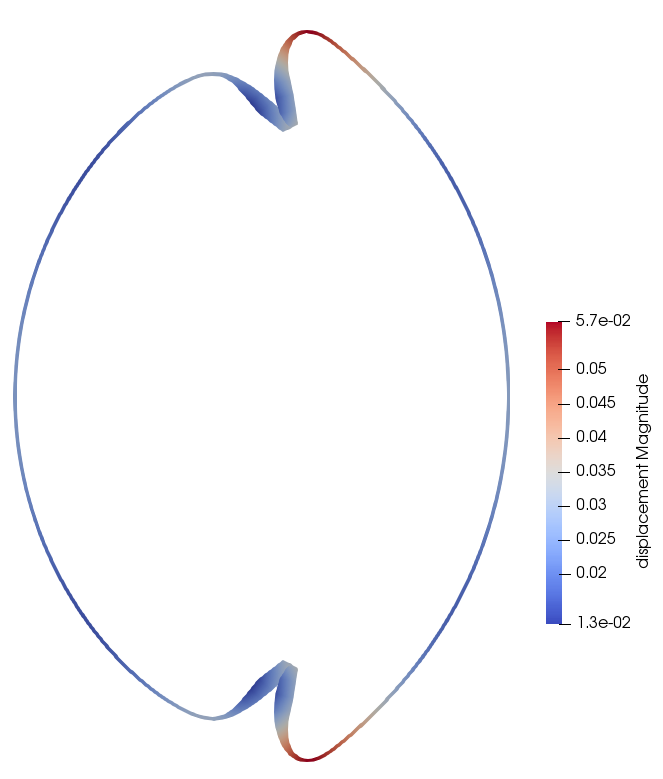
\includegraphics[width=0.9\textwidth]{instab_test_1_membrane_inv_cells.png}
\caption{After numerical failure}
\label{fig:3.16.2}
\end{subfigure}
\begin{subfigure}{0.38\textwidth}
\centering
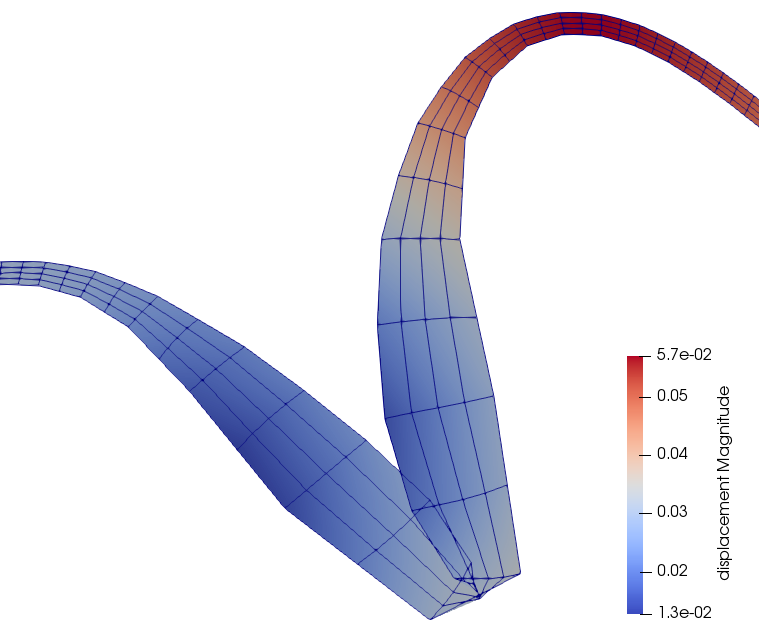
\includegraphics[width=0.9\textwidth]{instab_test_1_membrane_disp.png}
\caption{Zoomed view of inverted elements in membrane (top section at $\Theta = \ang{90}$)}
\label{fig:3.16.3}
\end{subfigure}
\caption{Magneto-elastic membrane during numerical failure}
\label{fig:3.16}
\end{figure}

We examine the results for the magneto-elastic membrane in \Cref{fig:3.16}. For the considered load values, material parameters and membrane thickness, we observe a numerical failure of the employed (direct coupled) solution method. The result in \Cref{fig:3.16.1} is at the end of the magnetic loading, i.e. end of the first phase of loading. The numerical failure observed in \Cref{fig:3.16.2} is at the first load step of the second phase of loading, i.e. the mechanical inflating pressure load application. The membrane appears to buckle at the large pressure applied in the first step on the new compressed (oval) geometry structure. The buckling of the membrane occurs at the sections located along the longitudinal axes at $\Theta = \ang{90}$ and $\Theta = \ang{270}$. On close examination of the elements in these sections, we observe inverted elements at the region near the kink in \Cref{fig:3.16.3}. \par 

\begin{figure}[h]
\centering
\begin{subfigure}{0.4\textwidth}
\centering
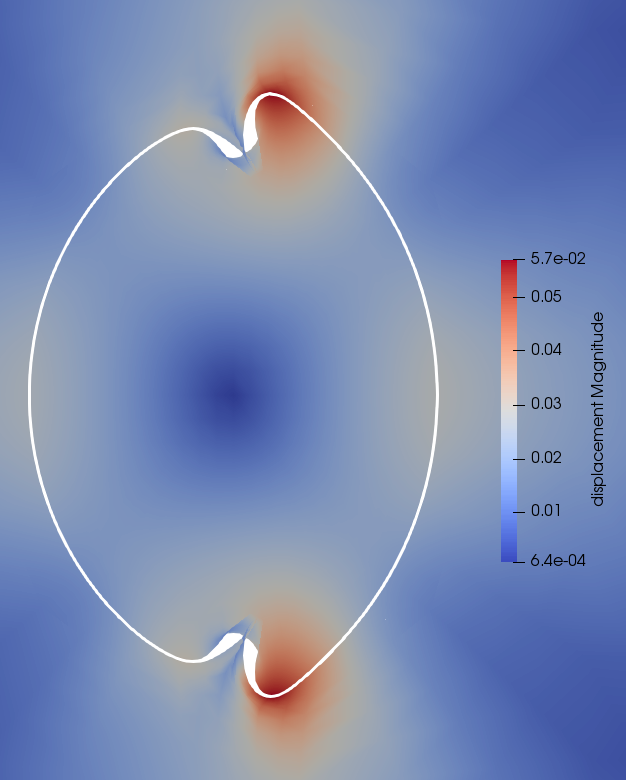
\includegraphics[width=0.9\textwidth]{instab_test_1_inv_cells.png}
\caption{After numerical failure}
\label{fig:3.17.1}
\end{subfigure}
\begin{subfigure}{0.58\textwidth}
\centering
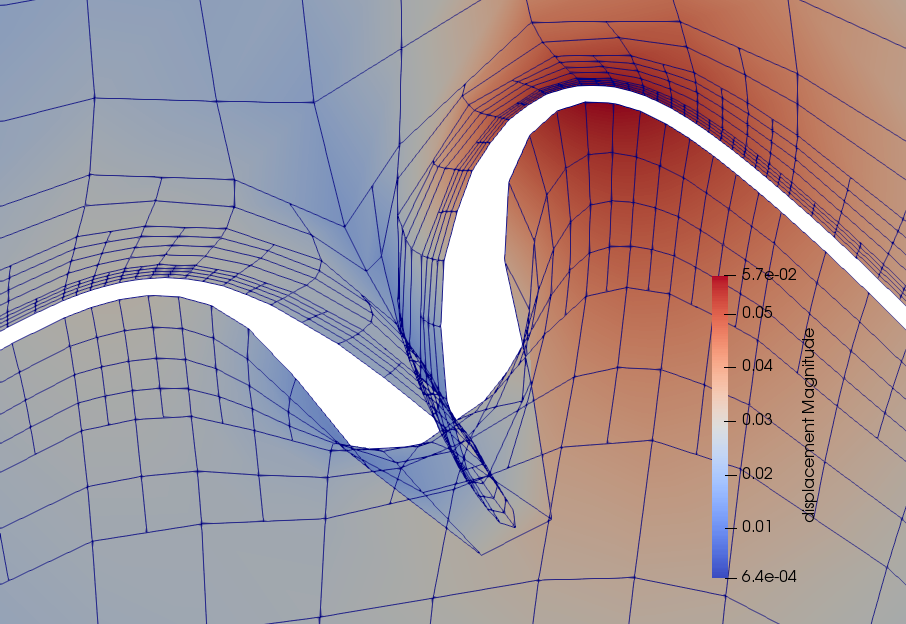
\includegraphics[width=0.9\textwidth]{instab_test_1_free_space_inv_cells.png}
\caption{Zoomed view of inverted elements in free space (top section at $\Theta = \ang{90}$)}
\label{fig:3.17.2}
\end{subfigure}
\caption{Free space elements surrounding the membrane causing the numerical failure (white section is the cut-out membrane for better visualization purpose)}
\label{fig:3.17}
\end{figure}

We now focus on the elements in the free space neighbouring the membrane where we observed numerical failure. It is important to note that the free space material is modelled as a very complaint elastic body with elastic stiffness relatively low compared to the membrane's stiffness. Observing \Cref{fig:3.17.2}, it is suspected that the cause of the numerical failure is the inversion of elements in the complaint free space with non-invertible deformation maps $\bm{\varphi}$. One can clearly observe the outer free space elements have intersected with the inner free space elements, thus crossing the membrane region (white cut-out section). The reason for this numerical failure is due to the direct solution of the coupled problem, solving for both the magneto-elastic membrane as well as the complaint free space together. Use of a segregated solution method can be motivated to overcome this failure in modelling buckling of the membrane. In the segregated approach, one splits the solution to the problem of deformable geometry (in our case the magneto-elastic membrane) from the mesh update of the surrounding free space. In the first stage, one would consider the degrees of freedom in membrane only and solve the coupled problem for finite deformations of the magneto-elastic body without considering the free space degrees of freedom. In the next stage, which is termed as \textbf{moving-mesh update} in literature \cite{bustamante2011numerical} and \cite{pelteret2016} for the magneto-active polymers, one would then use the solution of the first stage coupled problem as the necessary inhomogeneous Dirichlet boundary conditions and solve another boundary value problem to compute a suitable deformation map $\bm{\varphi}$ in the free space $\mathcal{S}_0$. Such techniques were developed for problems in fluid mechanics and fluid-structure interaction problems where large deformations and moving domains, boundaries and interfaces are to be modelled accurately. Employing this staggered algorithm, one could then truly be able to move past the critical point of buckling as observed in above results for the failing simulations. Due to time restrictions to submit the thesis report, the work in the direction to implement such a mesh update algorithm could not be done and presented in this report. Readers interested to know more about the staggered approach are directed to \cite[see][Sec. 7]{pelteret2016} and the references mentioned therein. \par 

